% Options for packages loaded elsewhere
\PassOptionsToPackage{unicode,pdfpagelabels}{hyperref}
\PassOptionsToPackage{hyphens}{url}
\PassOptionsToPackage{dvipsnames,svgnames,x11names}{xcolor}
%
\documentclass[
  14pt,
  a4paper,
  oneside,
  open=any,
  a4paper,
  14pt]{report}

\usepackage{amsmath,amssymb}
\usepackage{iftex}
\ifPDFTeX
  \usepackage[T1]{fontenc}
  \usepackage[utf8]{inputenc}
  \usepackage{textcomp} % provide euro and other symbols
\else % if luatex or xetex
  \usepackage{unicode-math}
  \defaultfontfeatures{Scale=MatchLowercase}
  \defaultfontfeatures[\rmfamily]{Ligatures=TeX,Scale=1}
\fi
\usepackage[]{lmodern}
\ifPDFTeX\else  
    % xetex/luatex font selection
\fi
% Use upquote if available, for straight quotes in verbatim environments
\IfFileExists{upquote.sty}{\usepackage{upquote}}{}
\IfFileExists{microtype.sty}{% use microtype if available
  \usepackage[]{microtype}
  \UseMicrotypeSet[protrusion]{basicmath} % disable protrusion for tt fonts
}{}
\makeatletter
\@ifundefined{KOMAClassName}{% if non-KOMA class
  \IfFileExists{parskip.sty}{%
    \usepackage{parskip}
  }{% else
    \setlength{\parindent}{0pt}
    \setlength{\parskip}{6pt plus 2pt minus 1pt}}
}{% if KOMA class
  \KOMAoptions{parskip=half}}
\makeatother
\usepackage{xcolor}
\usepackage[top=2.5cm,bottom=2.5cm,left=1cm,right=1cm,marginparsep=2cm]{geometry}
\setlength{\emergencystretch}{3em} % prevent overfull lines
\setcounter{secnumdepth}{5}
% Make \paragraph and \subparagraph free-standing
\makeatletter
\ifx\paragraph\undefined\else
  \let\oldparagraph\paragraph
  \renewcommand{\paragraph}{
    \@ifstar
      \xxxParagraphStar
      \xxxParagraphNoStar
  }
  \newcommand{\xxxParagraphStar}[1]{\oldparagraph*{#1}\mbox{}}
  \newcommand{\xxxParagraphNoStar}[1]{\oldparagraph{#1}\mbox{}}
\fi
\ifx\subparagraph\undefined\else
  \let\oldsubparagraph\subparagraph
  \renewcommand{\subparagraph}{
    \@ifstar
      \xxxSubParagraphStar
      \xxxSubParagraphNoStar
  }
  \newcommand{\xxxSubParagraphStar}[1]{\oldsubparagraph*{#1}\mbox{}}
  \newcommand{\xxxSubParagraphNoStar}[1]{\oldsubparagraph{#1}\mbox{}}
\fi
\makeatother
\pagestyle{plain}

\providecommand{\tightlist}{%
  \setlength{\itemsep}{0pt}\setlength{\parskip}{0pt}}\usepackage{longtable,booktabs,array}
\usepackage{calc} % for calculating minipage widths
% Correct order of tables after \paragraph or \subparagraph
\usepackage{etoolbox}
\makeatletter
\patchcmd\longtable{\par}{\if@noskipsec\mbox{}\fi\par}{}{}
\makeatother
% Allow footnotes in longtable head/foot
\IfFileExists{footnotehyper.sty}{\usepackage{footnotehyper}}{\usepackage{footnote}}
\makesavenoteenv{longtable}
\usepackage{graphicx}
\makeatletter
\newsavebox\pandoc@box
\newcommand*\pandocbounded[1]{% scales image to fit in text height/width
  \sbox\pandoc@box{#1}%
  \Gscale@div\@tempa{\textheight}{\dimexpr\ht\pandoc@box+\dp\pandoc@box\relax}%
  \Gscale@div\@tempb{\linewidth}{\wd\pandoc@box}%
  \ifdim\@tempb\p@<\@tempa\p@\let\@tempa\@tempb\fi% select the smaller of both
  \ifdim\@tempa\p@<\p@\scalebox{\@tempa}{\usebox\pandoc@box}%
  \else\usebox{\pandoc@box}%
  \fi%
}
% Set default figure placement to htbp
\def\fps@figure{htbp}
\makeatother

\usepackage{geometry}       % Control page margins
\usepackage{setspace}       % Custom line spacing
\usepackage{titlesec}       % Modern section titles
\usepackage{amsmath}        % Math environments
\usepackage{amssymb}        % Math symbols
\usepackage{amsfonts}       % Math fonts
\usepackage{amsthm}         % Math theorems
\usepackage{unicode-math}
\usepackage{mathtools}      % Extra math tools
\usepackage{array}          % For custom column widths in tables
\renewcommand{\arraystretch}{1.5}
\usepackage{derivative}
\usepackage{physics2}
\usephysicsmodule{qtext.legacy}
\usepackage{siunitx}        % SI units
\sisetup{per-mode = symbol} % Set SI unit fractions to use a solidus
\usepackage{commath}        % For derivatives
\usepackage{graphicx}       % For including images
\usepackage{xcolor}         % Color text, if needed
\usepackage{xparse}
\usepackage{booktabs}       % Improved tables
\usepackage{enumitem}       % Customized lists
\usepackage{float}          % Improved figure placement
\usepackage{tikz}           % Core TikZ package
\usetikzlibrary{positioning, arrows.meta}
\usepackage{circuitikz}     % For circuits!
\usepackage{pgfplots}       % For plots
\pgfplotsset{compat=1.18}   % Set compatibility to 1.18
\usepgfplotslibrary{groupplots,units}
\usepackage[pgf]{bodeplot}
\usepackage{fancyhdr}       % Customize headers and footers
\usepackage{appendix}       % Appendices
\usepackage{cancel}         % Cancel terms in equations
\usepackage[most]{tcolorbox}
\usepackage{mdframed}       % Framed text blocks
% Document navigation
\usepackage{tabularray}
\usepackage[pdfpagelabels]{hyperref}       % For clickable links and cross-references
\usepackage{bookmark}       % Improved bookmarks for navigation
\AtBeginDocument{\RenewCommandCopy\qty\SI}
% spacing and margins
% Header and footer settings
\fancypagestyle{plain}{%
  \fancyhf{}%
  \fancyhead[L]{\textbf{Nicholas Russell}}%
  \fancyhead[C]{ELECTENG 332: Control Systems Notes}%
  \fancyhead[R]{October 23rd, 2024}%
  \fancyfoot[R]{\thepage}%
  \renewcommand{\headrulewidth}{0.4pt}%
  \renewcommand{\footrulewidth}{0pt}%
}
\pagestyle{plain}
\renewcommand{\theequation}{\arabic{equation}}
% Define colors
\definecolor{borderblue}{HTML}{0099FF} % #0099FF
\definecolor{boxheadcol}{HTML}{D6D6F0} % #D6D6F0
\definecolor{boxbodycol}{HTML}{EBEBF7} % #EBEBF7
% Custom macros
\DeclareSIUnit{\rads}{\radian\per\second}
\newcommand{\bluetext}[1]{\textcolor{blue}{#1}}
\newcommand{\redtext}[1]{\textcolor{red}{#1}}
\DeclareDocumentCommand\flatfrac{ m m }{\left.#1\middle\slash#2\right.}
\newcolumntype{Y}{>{\centering\arraybackslash}X}
\makeatletter
\@ifpackageloaded{tcolorbox}{}{\usepackage[skins,breakable]{tcolorbox}}
\@ifpackageloaded{fontawesome5}{}{\usepackage{fontawesome5}}
\definecolor{quarto-callout-color}{HTML}{909090}
\definecolor{quarto-callout-note-color}{HTML}{0758E5}
\definecolor{quarto-callout-important-color}{HTML}{CC1914}
\definecolor{quarto-callout-warning-color}{HTML}{EB9113}
\definecolor{quarto-callout-tip-color}{HTML}{00A047}
\definecolor{quarto-callout-caution-color}{HTML}{FC5300}
\definecolor{quarto-callout-color-frame}{HTML}{acacac}
\definecolor{quarto-callout-note-color-frame}{HTML}{4582ec}
\definecolor{quarto-callout-important-color-frame}{HTML}{d9534f}
\definecolor{quarto-callout-warning-color-frame}{HTML}{f0ad4e}
\definecolor{quarto-callout-tip-color-frame}{HTML}{02b875}
\definecolor{quarto-callout-caution-color-frame}{HTML}{fd7e14}
\makeatother
\makeatletter
\@ifpackageloaded{bookmark}{}{\usepackage{bookmark}}
\makeatother
\makeatletter
\@ifpackageloaded{caption}{}{\usepackage{caption}}
\AtBeginDocument{%
\ifdefined\contentsname
  \renewcommand*\contentsname{Table of contents}
\else
  \newcommand\contentsname{Table of contents}
\fi
\ifdefined\listfigurename
  \renewcommand*\listfigurename{List of Figures}
\else
  \newcommand\listfigurename{List of Figures}
\fi
\ifdefined\listtablename
  \renewcommand*\listtablename{List of Tables}
\else
  \newcommand\listtablename{List of Tables}
\fi
\ifdefined\figurename
  \renewcommand*\figurename{Figure}
\else
  \newcommand\figurename{Figure}
\fi
\ifdefined\tablename
  \renewcommand*\tablename{Table}
\else
  \newcommand\tablename{Table}
\fi
}
\@ifpackageloaded{float}{}{\usepackage{float}}
\floatstyle{ruled}
\@ifundefined{c@chapter}{\newfloat{codelisting}{h}{lop}}{\newfloat{codelisting}{h}{lop}[chapter]}
\floatname{codelisting}{Listing}
\newcommand*\listoflistings{\listof{codelisting}{List of Listings}}
\makeatother
\makeatletter
\@ifpackageloaded{tikz}{}{\usepackage{tikz}}
\makeatother
\makeatletter
\@ifpackageloaded{caption}{}{\usepackage{caption}}
\@ifpackageloaded{subcaption}{}{\usepackage{subcaption}}
\makeatother

\usepackage{hyphenat}
\usepackage{ifthen}
\usepackage{calc}
\usepackage{calculator}



\usepackage{graphicx}
\usepackage{geometry}
\usepackage{afterpage}
\usepackage{tikz}
\usetikzlibrary{calc}
\usetikzlibrary{fadings}
\usepackage[pagecolor=none]{pagecolor}


% Set the titlepage font families







% Set the coverpage font families


\usepackage{bookmark}

\IfFileExists{xurl.sty}{\usepackage{xurl}}{} % add URL line breaks if available
\urlstyle{same} % disable monospaced font for URLs
\hypersetup{
  pdftitle={ELECTENG 332: Control Systems},
  pdfauthor={Nicholas Russell},
  colorlinks=true,
  linkcolor={blue},
  filecolor={Maroon},
  citecolor={Blue},
  urlcolor={Blue},
  pdfcreator={LaTeX via pandoc}}


\title{ELECTENG 332: Control Systems}
\usepackage{etoolbox}
\makeatletter
\providecommand{\subtitle}[1]{% add subtitle to \maketitle
  \apptocmd{\@title}{\par {\large #1 \par}}{}{}
}
\makeatother
\subtitle{Lecture Notes}
\author{Nicholas Russell}
\date{Wednesday, October 23, 2024}

\begin{document}
%%%%% begin titlepage extension code


\begin{titlepage}

%%% TITLE PAGE START

% Set up alignment commands
%Page
\newcommand{\titlepagepagealign}{
\ifthenelse{\equal{center}{right}}{\raggedleft}{}
\ifthenelse{\equal{center}{center}}{\centering}{}
\ifthenelse{\equal{center}{left}}{\raggedright}{}
}


\newcommand{\titleandsubtitle}{
% Title and subtitle
{{\huge{\bfseries{\nohyphens{ELECTENG 332: Control Systems}}}}\par
}%

\vspace{\betweentitlesubtitle}
{
{\Large{\nohyphens{Lecture Notes}}}\par
}}
\newcommand{\titlepagetitleblock}{
\newcommand{\HRule}{\rule{\linewidth}{0.5mm}} 

\HRule\\[0.4cm]

\titleandsubtitle

\HRule\\
}
\newcommand{\authorstyle}[1]{{\large{#1}}}

\newcommand{\affiliationstyle}[1]{{\large{#1}}}

\newcommand{\titlepageauthorblock}{
{\authorstyle{
Nicholas Russell\\University of Auckland\\Department of Electrical,
Computer, and Software Engineering}}}

\newcommand{\titlepageaffiliationblock}{}
\newcommand{\headerstyled}{%
{\textsc{\LARGE{}}}
}
\newcommand{\footerstyled}{%
{}
}
\newcommand{\datestyled}{%
{\large{Wednesday, October 23, 2024}}
}


\newcommand{\titlepageheaderblock}{\headerstyled}

\newcommand{\titlepagefooterblock}{
\footerstyled
}

\newcommand{\titlepagedateblock}{
\datestyled
}

%set up blocks so user can specify order
\newcommand{\titleblock}{\newlength{\betweentitlesubtitle}
\setlength{\betweentitlesubtitle}{\baselineskip}
{

{\titlepagetitleblock}
}

\vspace{1.5cm}
}

\newcommand{\authorblock}{{\titlepageauthorblock}

\vspace{1cm}
}

\newcommand{\affiliationblock}{{\titlepageaffiliationblock}

\vspace{0pt}
}

\newcommand{\logoblock}{{
\includegraphics[width=0.8\textwidth]{images/DECSE-HC-4C-01.png}}

\vspace{2\baselineskip}
}

\newcommand{\footerblock}{}

\newcommand{\dateblock}{{\titlepagedateblock}

\vspace{0pt}
}

\newcommand{\headerblock}{}

\thispagestyle{empty} % no page numbers on titlepages


\newlength{\minipagewidth}
\setlength{\minipagewidth}{\textwidth}
\raggedright % single minipage
% [position of box][box height][inner position]{width}
% [s] means stretch out vertically; assuming there is a vfill
\begin{minipage}[b][\textheight][s]{\minipagewidth}
\titlepagepagealign
\headerblock

\logoblock

\titleblock

\authorblock

\vfill

\dateblock
\par

\end{minipage}\ifthenelse{\equal{}{right} \OR \equal{}{leftright} }{
\hspace{\B}
\vrulecode}{}
\clearpage
%%% TITLE PAGE END
\end{titlepage}
\setcounter{page}{1}

%%%%% end titlepage extension code

\renewcommand*\contentsname{Table of contents}
{
\hypersetup{linkcolor=}
\setcounter{tocdepth}{3}
\tableofcontents
}
\listoffigures

\bookmarksetup{startatroot}

\chapter*{Introduction}\label{introduction}

\markboth{Introduction}{Introduction}

\begin{quote}
\emph{Dear god not another one of these.}
\end{quote}

This is my ``coursebook'', or rather, a collection of notes for the
course ELECTENG 332: Control Systems. The notes are written in Quarto, a
markdown-based document processor that supports LaTeX and code blocks,
and requires this introduction file.

Please skip this bit, there's nothing to see here.

\part{Akshya's Content}

\chapter{Basics of Signals and
Systems}\label{basics-of-signals-and-systems}

\section*{Learning Outcomes}\label{learning-outcomes}
\addcontentsline{toc}{section}{Learning Outcomes}

\markright{Learning Outcomes}

After completing this module, you should be able to:

\begin{enumerate}
\def\labelenumi{\arabic{enumi}.}
\item
  Understand the uniqueness of the exponential function
\item
  Understand the concept of engineering infinity
\item
  Understand the concept of complex frequency
\item
  Understand the concept of signals, and be able to classify them
\item
  Understand the concept of systems, and be able to classify them
\item
  Understand the concept of control systems
\end{enumerate}

\section{The Importance of the Exponential
Function}\label{the-importance-of-the-exponential-function}

The Exponential function, written as either \(e^{ax}\) or \(e^{at}\)
depending on whether it is \(f(t)\) or \(f(x)\), has properties that
make it mathematically unique.

\begin{enumerate}
\def\labelenumi{\arabic{enumi}.}
\tightlist
\item
  The derivative (rate of change) of the exponential function is the
  exponential function itself. More generally, this is a function whose
  rate of change is proportional to the function itself.
\end{enumerate}

\begin{equation}\phantomsection\label{eq-exp-derivative}{
    \odv{e^{ax}}{x} = a e^{ax}
}\end{equation}

\begin{enumerate}
\def\labelenumi{\arabic{enumi}.}
\setcounter{enumi}{1}
\tightlist
\item
  The integral of the exponential function is also the exponential
  function itself.
\end{enumerate}

\begin{equation}\phantomsection\label{eq-exp-integral}{
    \int e^{ax} \odif{x} = \dfrac{1}{a} e^{ax} 
}\end{equation}

\section{The Concept of Engineering
Infinity}\label{the-concept-of-engineering-infinity}

Consider a signal \(e^{-at}\). The time constant for this signal is
\(T = \dfrac{1}{a}\). Theoretically, the signal is meant to decay to
zero as time approaches infinity, i.e.

\begin{equation}\phantomsection\label{eq-engineering-infinity}{
    \lim\limits_{t \to \infty} e^{-at} = 0  
}\end{equation}

But in practice, this is not the case, as its value will be very, very
small after five time constants \(5T\) (or \(5\tau\)). This is the
\textcolor{red}{\textbf{\emph{Concept of Engineering Infinity}}}. The
signal will never reach zero, but it will be so small that it can be
considered zero for all practical purposes. This is a very important
concept in control systems, as it allows us to simplify our calculations
and analysis.

\section{The Concept of Complex
Frequency}\label{the-concept-of-complex-frequency}

Complex frequency is found commonly in electrical engineering. It is
often notated as \(j\omega\) or \(s = \sigma \pm j\omega\). These
frequencies always come in pairs, so the use of \(\pm\) is implicit to
this, as complex numbers have complex conjugates (normally notated by
\(z^*\) or \(\bar{z}\)). i.e.~\(s = \sigma + j\omega\) has the conjugate
\(s=\sigma - j\omega\). This is backed up by De Moivre's formula which
is defined mathematically as:

\begin{equation}\phantomsection\label{eq-de-moivre}{
\begin{gathered}
    \forall x \in \mathbb{R}\qcomma\forall n \in \mathbb{Z} \\
    e^{jnx} = \cos(n x) + j \sin(n x)  
\end{gathered}
}\end{equation}

Or more generally for our applications (this is also known as Euler's
formula):

\begin{equation}\phantomsection\label{eq-euler}{
\begin{gathered}
    e^{jx} = \cos(x) + j \sin(x) \\
    \text{Where}\; x \in \mathbb{R} \\
    \text{and}\; j \equiv i = \sqrt{-1}
\end{gathered}
}\end{equation}

This means that:

\begin{quote}
\textcolor{red}{A complex frequency \(j\omega\) represents a pure
sinusoidal signal of frequency \(\omega\;\unit{\radian\per\second}\)}
\end{quote}

For example, if a signal has a complex frequency
\(\complexqty[output-complex-root=j, complex-root-position=before-number]{314i}{\radian\per\second}\),
then this responds to a pure sinusoid of frequency
\(\SI{314}{\radian\per\second}\) (i.e.~\(\SI{50}{\hertz}\)).

Furthermore:

\begin{quote}
\textcolor{red}{A complex frequency \(s = \sigma + j\omega\) represents
an exponentially damped signal of frequency
\(j\omega\;\unit{\radian\per\second}\), and decays/amplifies at a rate
decided by \(\sigma\)}
\end{quote}

\section{What are Signals?}\label{what-are-signals}

\subsection{Introduction}\label{introduction-1}

It is difficult to find a unique definition of a signal. However in the
context of this course, we give a workable definition which suits most
of out purposes as:

\begin{quote}
\textcolor{red}{A Signal conveys information about a physical phenomenon
which evolves in time or space.}
\end{quote}

Examples of such signals include: Voltage, Current, Speech, Television,
Images from remote space probes, Voltages generated by the heart and
brain, Radar and Sonar echoes, Seismic vibrations, Signals from GPS
satellites, Signals from human genes, and countless other applications.

\subsection{Energy and Power Signals}\label{energy-and-power-signals}

\textbf{Energy Signals}

\begin{quote}
\textcolor{red}{A signal is said to be an energy signal if and only if
it has finite energy.}
\end{quote}

\textbf{Power Signals}

\begin{quote}
\textcolor{blue}{A signal is said to be a power signal if and only if
the average power of the signal is finite and non-zero.}
\end{quote}

\textbf{Instantaneous Power}

\begin{quote}
The instantaneous power \(p(t)\) of a signal \(x(t)\) is expressed as:
\begin{equation}\phantomsection\label{eq-instantaneous-power-def}{
p(t) = x^2(t)
}\end{equation}
\end{quote}

\textbf{Continuous-Time Signal Energy}

\begin{quote}
The total energy of a continuous-time signal \(x(t)\) is given by:
\end{quote}

\[
    E = \lim\limits_{T \to \infty}\int\limits_{-T/2}^{T/2} x^2(t) \odif{t} = \int\limits_{-\infty}^{\infty} x^2(t) \odif{t}
\]

\textbf{Complex Valued Signal Energy}

\begin{quote}
For a complex valued signal:
\end{quote}

\[
    E = \int\limits_{-\infty}^{\infty} \abs{x(t)}^2 \odif{t}
\]

\textbf{Average Power}

\begin{quote}
Since power equals to the time average of the energy, the average power
is given by: \[
P = \lim\limits_{T \to \infty} \dfrac{1}{T} \int\limits_{-T/2}^{T/2} x^2(t) \odif{t} = \dfrac{E}{T}
\]
\end{quote}

Note that during calculation of energy, we average the power over an
indefinitely large interval.

\begin{quote}
\textcolor{red}{A signal with finite energy has zero power and a signal
with finite power has infinite energy.}
\end{quote}

Furthermore, some additional concepts of note:

\begin{enumerate}
\def\labelenumi{\alph{enumi}.}
\item
  A signal can not both be an energy and a power signal. This
  classification of signals based on power and energy are mutually
  exclusive.
\item
  However, a signal can belong to neither of the above two categories.
\item
  The signals which are both deterministic and non-periodic have finite
  energy and therefore are energy signals. Most of this signals, in
  practice, belong to this category.
\item
  Periodic signals and random signals are essentially power signals.
\item
  Periodic signals for which the area under \(\abs{x(t)}^2\) over one
  period is finite are energy signals.
\end{enumerate}

\subsection{Examples}\label{examples}

\subsubsection{Unit Step Function}\label{unit-step-function}

Consider a unit step function defined as:
\begin{equation}\phantomsection\label{eq-unit-step-function-example}{
    u(t) =         
    \begin{cases}             
        1 & t \geq 0         \\             
        0 & \text{otherwise}         
    \end{cases}
}\end{equation}

Determine whether this is an energy signal or a power signal or neither.

\textbf{Solution:} Let us compute the energy of this signal as:

\begin{equation}\phantomsection\label{eq-unit-step-energy}{
    E = \int\limits_{-\infty}^{\infty} {[u(t)]}^2 \odif{t} = \int\limits_{0}^{\infty} {[0]}^2 \odif{t} = \int\limits_{0}^{\infty} {[1]}^2 \odif{t} = \infty 
}\end{equation}

Since the energy of this signal is infinite, it cannot be an energy
signal. Let us compute the power of this signal as:

\begin{equation}\phantomsection\label{eq-unit-step-power}{
    P = \lim\limits_{T \to \infty} \dfrac{1}{T} \int\limits_{-T/2}^{T/2} {[u(t)]}^2 \odif{t} = \lim\limits_{T \to \infty} \dfrac{1}{T} \int\limits_{0}^{T/2} {[u(t)]}^2 \odif{t} = \dfrac{1}{2}
}\end{equation}

The power of this signal is finite. Hence, \textcolor{red}{this is a
power signal}.

\subsubsection{Exponential Function}\label{exponential-function}

Consider an exponential function defined as:

\begin{equation}\phantomsection\label{eq-exp-function-example}{
    x(t) = e^{-at}u(t)\qqtext{where} u(t) \text{ is the unit step signal}, \; a > 0 
}\end{equation}

Classify this signal as an energy, power, or neither.

\textbf{Solution:} Let us compute the energy of this signal as:

\begin{equation}\phantomsection\label{eq-exp-function-energy}{
    E = \int\limits_{-\infty}^{\infty} {[x(t)]}^2  \odif{t} = \int\limits_{0}^{\infty} {[e^{-at}]}^2 \odif{t} = \int\limits_{0}^{\infty} e^{-2at} \odif{t} = \dfrac{1}{2a} < \infty 
}\end{equation}

Thus, \(x(t) = e^{-at} u(t)\) is an \textcolor{red}{energy signal}.

\subsubsection{Ramp Function}\label{ramp-function}

Consider a ramp function defined as:

\begin{equation}\phantomsection\label{eq-ramp-function-example}{
    r(t) = 
    \begin{cases}         
        At & t \geq 0         \\         
        0  & \text{otherwise}     
    \end{cases} 
}\end{equation}

Classify this signal as an energy, power, or neither.

\textbf{Solution:} Let us compute the energy of this signal as:

\begin{equation}\phantomsection\label{eq-ramp-function-energy}{
    E = \int\limits_{-\infty}^{\infty} {r(t)}^2 \odif{t} = \int\limits_{-\infty}^{0} {[0]}^2 \odif{t} = \int\limits_{0}^{\infty} A^2 t^2 \odif{t} = A^2 \dfrac{T^3}{3} \Bigg|_{0}^{\infty} = \infty 
}\end{equation}

Since the energy of this signal is infinite, it cannot be an energy
signal. Let us compute the power of this signal as:

\begin{equation}\phantomsection\label{eq-ramp-function-power}{
    P = \lim\limits_{T \to \infty} \dfrac{1}{T} \int\limits_{-T/2}^{T/2} {[r(t)]}^2 \odif{t} = \lim\limits_{T \to \infty} \dfrac{1}{T} \int\limits_{0}^{T/2} A^2 t^2 \odif{t} = A^2 \lim\limits_{T \to \infty} \dfrac{1}{T} \dfrac{T^3}{3} \Bigg|_{0}^{\infty} = \infty 
}\end{equation}

The power of this signal is infinite. Hence, this is
\textcolor{red}{neither a power nor an energy signal}.

\section{What are Systems?}\label{what-are-systems}

\subsection{Introduction}\label{introduction-2}

The term \emph{system} is derived from the Greek word \emph{systema},
which means an organised relationship among functioning units or
components. It is often used to describe any orderly arrangement of
ideas or constructs.

According to the Webster's dictionary:

\begin{quote}
\textcolor{blue}{``A system is an aggregation or assemblage of objects
united by some form of regular interaction or interdependence; a group
of diverse units so combined by nature or art as to form an integral;
whole and to function, operate, or move in unison and often in obedience
to some form of control\ldots{}''}
\end{quote}

According to the International Council on Systems Engineering (INCOSE):

\begin{quote}
\textcolor{red}{``A system is an arrangement of parts or elements that
together exhibit behaviour or meaning that the individual constituents
do not.''} The elements or parts, can include people, hardware,
software, facilities, policies, and documents; that is, all things
required to produce system-level results.
\end{quote}

It is difficult to give a single and precise definition of the term
system, which will suit to different perspectives of different people.
In practice, what is meant by ``the system'' depends on the objectives
of a particular study.

From the control engineering perspective, \textcolor{red}{the system is
any interconnection of components to achieve desired objectives.} It is
characterised by its \textcolor{blue}{Inputs, Outputs,} and the rules of
operations or laws. For example:

\begin{enumerate}
\def\labelenumi{\alph{enumi}.}
\item
  The laws of operation in electrical systems are Ohm's law, which gives
  the voltage-current relationships for resistors, capacitors and
  inductors, and Kirchhoff's laws, which govern the laws of
  interconnection of various electrical components.
\item
  Similarly, in mechanical systems, the laws of operation are Newton's
  laws. These laws can be used to derive mathematical models of the
  system.
\end{enumerate}

\subsection{The System as an Operator}\label{the-system-as-an-operator}

A system is defined mathematically as a transformation which maps an
input signal \(x(t)\) to an output signal \(y(t)\). For a continuous
time system, the input-output mapping is expressed as:

\begin{equation}\phantomsection\label{eq-system-operator}{
    \textcolor{red}{y(t) = \mathcal{S}[x(t)]}
}\end{equation}

where \(\mathcal{S}\) is the system operator.

\textcolor{red}{A Control system may be defined as an interconnection of
components which are configured to provide a desired response.}

\subsection{Classification of Systems}\label{classification-of-systems}

The basis of classifying systems are many. They can be classified
according to the following:

\begin{enumerate}
\def\labelenumi{\alph{enumi}.}
\item
  The Time Frame: \emph{(discrete, continuous or hybrid)};
\item
  System Complexity: \emph{(physical, conceptual and esoteric)};
\item
  Uncertainties: \emph{(deterministic and stochastic)};
\item
  Nature and type of components: \emph{(static or dynamic, linear or
  nonlinear, time-invariant or time variant, lumped or distributed
  etc)};
\end{enumerate}

\begin{enumerate}
\def\labelenumi{\arabic{enumi}.}
\tightlist
\item
  Linear and nonlinear systems
\item
  Time-invariant and time-variant systems
\item
  Static (memory-less) and dynamic (with memory) systems
\item
  Causal and Non-causal systems
\item
  Lumped and distributed parameter systems
\item
  Deterministic and stochastic systems
\item
  Continuous and discrete systems
\end{enumerate}

\subsection{Linear and Nonlinear
Systems}\label{linear-and-nonlinear-systems}

A system is said to be linear provided it satisfies the principle of
superposition which is the combination of the additive and homogeneity
properties. Otherwise, it is nonlinear.

\subsubsection{Principle of Additivity}\label{principle-of-additivity}

\subsubsection{Principle of Homogeneity or
Scaling}\label{principle-of-homogeneity-or-scaling}

\subsubsection{Principle of
Superposition}\label{principle-of-superposition}

\subsection{Time-Invariant and Time-Variant
Systems}\label{time-invariant-and-time-variant-systems}

\subsection{Static and Dynamic
Systems}\label{static-and-dynamic-systems}

\subsection{Causal and Non-Causal
Systems}\label{causal-and-non-causal-systems}

\section{What is a Control System?}\label{what-is-a-control-system}

\subsection{Introduction}\label{introduction-3}

\subsection{Common Terms of Control
Systems}\label{common-terms-of-control-systems}

\subsection{Classification of Control
Systems}\label{classification-of-control-systems}

\chapter{Mathematical Modeling of Dynamic
Systems}\label{mathematical-modeling-of-dynamic-systems}

\section*{Learning Outcomes}\label{learning-outcomes-1}
\addcontentsline{toc}{section}{Learning Outcomes}

\markright{Learning Outcomes}

After completing this module, you should be able to:

\begin{itemize}
\item
  Explain the purpose of mathematical models in analyzing and
  controlling dynamic systems, and identify the importance of modeling
  in engineering design and analysis.
\item
  Differentiate between differential equation models, transfer function
  models, and impulse response models, and recognize when each type is
  appropriate to use.
\item
  Develop mathematical models for electrical systems (RLC circuits) and
  mechanical systems (mass-spring-damper, rotational systems) by
  applying first principles.
\item
  Analyze the characteristics of a system using poles, zeros, and system
  order, and explain their physical significance in a transfer function.
\item
  Translate differential equation models to transfer functions using
  Laplace transforms and express these transfer functions in terms of
  poles and zeros for frequency-domain analysis.
\item
  Evaluate system responses to different types of inputs, including
  calculating zero-input, zero-state, and impulse responses for linear
  time-invariant systems.
\item
  Classify transfer functions as proper, strictly proper, bi-proper, or
  improper, and explain the implications of each classification for
  system behavior.
\item
  Apply the concepts of system modeling to solve practical problems,
  including calculating poles, zeros, and time constants, and using
  models to predict system responses to various inputs.
\end{itemize}

\begin{tcolorbox}[enhanced jigsaw, colframe=quarto-callout-important-color-frame, coltitle=black, colback=white, breakable, titlerule=0mm, rightrule=.15mm, arc=.35mm, bottomtitle=1mm, opacityback=0, toptitle=1mm, title=\textcolor{quarto-callout-important-color}{\faExclamation}\hspace{0.5em}{Philosophy Ahead!}, colbacktitle=quarto-callout-important-color!10!white, bottomrule=.15mm, toprule=.15mm, leftrule=.75mm, left=2mm, opacitybacktitle=0.6]

Some of the more philosophical concepts and ideas presented in this
chapter are not necessarily fact, nor are they to be taken as such. They
are also not examinable, but are added here to provide a broader
perspective on the more abstract concepts of modeling and system
dynamics.

\end{tcolorbox}

\section{Introduction}\label{introduction-4}

Loosely put, a model of a system is a tool we use to answer questions
about the system without having to conduct experimentation upon the
system itself. It is a collection of mathematical relationships between
system variables or process variables which purport to describe the
behaviour of the physical system being represented. It is a convenient
surrogate \& substitution for the real, physical system.

The main purpose of a model such as this, is to allow us to investigate
the system response. Primarilly, it allows us to analyze the system
under various input conditions, both rapidly and inexpensively, without
having to tamper with, or even have access to the physical entity. It
also allows us to analytically design controllers that can be used to
manipulate the system in a desired manner.

Determination of a mathematical model of a real world system is a
difficult task (see prior courses such as ENGSCI 111, 211 and 313, for
example, which are the ``Mathematical Modeling'' courses previously
sat.) in almost all fields of engineering and science. The difficulties
arise due to various reasons. Some of them include:

\begin{quote}
The diverse nature and complexities of dynamic systems. These range from
linear to non-linear; time-invariant to time-variant; lumped parameter
to distributed parameter and so on.
\end{quote}

A mathematical model should capture the underlying physics of the
system, and should define the cause and effect relationships between
various system variables/parameters in a quantitative manner. A model
should not be overcomplicated by including every phenomena that may
affect the system in microscopic detail, however. Doing so would make
the model unsuitable for analysis and controller design. On the other
hand, a model should not be oversimplified to the extent such that it
loses the dynamic resemblance to the original, physical, system. If this
were the case, the system model would be inaccurate and would result in
incorrect predictions.

For all intents and purposes, there are two approaches to find a model
for a given system that system designers commonly use.

\begin{enumerate}
\def\labelenumi{\arabic{enumi}.}
\item
  Break down the complex system into smaller components/elements/modules
  and establish a mathematical model for each of these elements using
  basic and fundamental physical laws/principles. This is known as the
  \textbf{\emph{first principles}} approach or a \textbf{\emph{first
  principles model}}. (You may be familiar with the term ``first
  principles'' from the prior course, ELECTENG 292, where Mark Andrews
  extensively reinforced the use of first principles in the analysis of
  problems from that course.)
\item
  Collect a set of input-output (I/O) data from the system by conducting
  experiments and process these using various techniques to establish a
  mathematical model. This approach comes under the purview of
  \textbf{\emph{system identification}}. In other words, F.A.F.O until
  something sticks.
\end{enumerate}

\begin{tcolorbox}[enhanced jigsaw, colframe=quarto-callout-important-color-frame, coltitle=black, colback=white, breakable, titlerule=0mm, rightrule=.15mm, arc=.35mm, bottomtitle=1mm, opacityback=0, toptitle=1mm, title=\textcolor{quarto-callout-important-color}{\faExclamation}\hspace{0.5em}{Important}, colbacktitle=quarto-callout-important-color!10!white, bottomrule=.15mm, toprule=.15mm, leftrule=.75mm, left=2mm, opacitybacktitle=0.6]

It is important to not confuse the use of models for the phenomena they
represent. A model can be thought of as an imaginary universe of sorts.
This universe is not a photograph or copy of reality; it captures the
aspects deemed necessary by the designer to be important enough to
consider. It is also to be of note that specific phenomena may also have
different models; Models can be numerous and many. Phenomena are one.

\begin{quote}
\textbf{A Map is not the Territory; A Map is the Model of the
Territory.}
\end{quote}

\end{tcolorbox}

\begin{quote}
Everything in the cosmos is energy and every object vibrates at certain
frequencies.
\end{quote}

When interpreted in a broad, metaphorical sense, the above statement
encapsulates the idea that \textbf{energy is a fundamental aspect of the
cosmos}, and everything, at its most fundamental and atomic level, can
be understood in terms of energy and vibrations. This idea is
``grounded'' both in physics and metaphysics.

\begin{quote}
Energy cannot be created or destroyed; it can only be changed from one
form to another. - Albert Einstein
\end{quote}

Einstein's research and discoveries in the fundamental nature of energy
and matter led to his most famous attribution, the equation:

\[
    E = mc^2
\]

which describes the relationship between energy and mass -- hence matter
-- and the interchangeability between them, and how they are
interconnected, not much unlike the two sides of a single coin. Some
more, ``out there'', perspectives and interpretations suggest the fact
that \textbf{everything in the universe is interconnected and resonates
with a universal energy or consciousness}. This perspective draws
heavily from Eastern philosophies, where the idea of interconnectedness
and vibrational energies is prevalent.

When an impulse disturbance is applied to an object or a system and left
to respond freely, it tends to vibrate preferentially at its
characteristic modes. These modes represent the natural frequencies at
which the system oscillates most efficiently. That is, every physical
object or system has a unique set of characteristic modes, which are the
frequencies at which it naturally oscillates when disturbed. These
frequencies are determined by the physical properties of the object,
such as its mass, stiffness, and shape.

In the context of the cosmos, various celestial bodies like planets,
stars, and even galaxies can exhibit natural frequencies of vibration.
These vibrations can arise from internal processes, such as seismic
activity within planets or oscillations in stars, or from external
influences, such as gravitational interactions between celestial bodies.

For stable systems, these characteristic modes decay exponentially and
eventually vanish as time approaches infinity. This does not mean that
these modes do not significantly affect the system behaviour and
response.

\begin{tcolorbox}[enhanced jigsaw, colframe=quarto-callout-note-color-frame, opacityback=0, leftrule=.75mm, colback=white, breakable, arc=.35mm, bottomrule=.15mm, rightrule=.15mm, left=2mm, toprule=.15mm]

\vspace{-3mm}\textbf{An Analogy}\vspace{3mm}

The seed of a plant contains all the genetic information necessary for
the development of the plant. It serves as the blueprint for the plant's
structure, growth pattern, and eventual form. The inherent
characteristics of a plant, such as its species, traits, and features,
are encoded within the seed. Similarly the dynamic behaviour of a system
are embedded in the characteristic modes.

\end{tcolorbox}

Physical Phenomena can be categorized essentially into two main groups:

\begin{enumerate}
\def\labelenumi{\arabic{enumi}.}
\tightlist
\item
  Energy dissipation
\item
  Energy absorption or storage
\end{enumerate}

Some Familiar models are:

\begin{enumerate}
\def\labelenumi{\roman{enumi}.}
\item
  Resistance, which models the phenomenon of energy dissipation.
\item
  Capacitance and Inductance, which model the phenomenon of energy
  absorption or storage.
\item
  Usually, Potential energy (related to displacement) is modeled by a
  capacitor \(\left(0.5CV^2=\dfrac{0.5Q^2}{C}\right)\) (by charge)
\item
  Kinetic energy (related to velocity; derivative of displacement) is
  modeled by an inductor \(\left(\dfrac{1}{2}LI^2\right)\) (by current;
  derivative of charge)
\end{enumerate}

\section{Concept of Static \& Dynamic Systems, and System
Order}\label{concept-of-static-dynamic-systems-and-system-order}

\subsection{Static Systems}\label{static-systems}

A static system does not have an energy storing element present, and
hence no memory. It is because of the absence of a memory element that
it is also referred to as a memoryless system. The response of a static
system to an input at a particular given time is dependent on only the
input at that given time. An example of a static system is a purely
resistive circuit.

\subsection{Dynamic Systems}\label{dynamic-systems}

A dynamic system, however, has at least, one energy storing element
present, and hence has a memory. Due to this, a dynamic system is often
referred to as a system with memory. The response of a dynamic system to
an input at a particular given time is dependant, not only on the input
at that given time, but also on the energy stored in the system's energy
storing elements, otherwise known as initial conditions. An example(s)
of a dynamic system is an RLC or RC or RL circuit.

\subsection{System Order}\label{system-order}

The order of a system is defined as being equal to the number of energy
storage elements present within the system. It can also be
mathematically interpreted as the highest power a derivative is raised
to in the model that describes the system, or in the s-domain, the
highest power of \(s\) in the transfer function of the system. For
example, a purely resistive circuit has no energy storage elements,
meaning that it is a system of order zero. A system with one energy
storage element, such as a RL or RC circuit, for example, has one energy
storage element (either an inductor or a capacitor), and is therefore a
system of order one. A system with two energy storage elements, such as
an RLC circuit, for example, is a system of order two. TL;DR: an
\(n\)-th order system has \(n\) energy storage elements.

\section{Differential Equation Models of Simple Dynamical
Systems}\label{differential-equation-models-of-simple-dynamical-systems}

We can map the input-output (I/O) relationships of systems such as
electrical, mechanical, hydraulic, and thermal systems via differential
equations. Irrespective of their complexity, each of these systems is
composed of a set of a few basic components, such as resistors,
capacitors, inductors, masses, springs, dampers, cross-sectional areas
of fluid tanks and thermal capacities. It is because of this, that we
can use approach 1, the first principles approach, to model these
systems given these basic components.

\section{Modeling of Electrical
Systems}\label{modeling-of-electrical-systems}

The basic elements, as most taking this course will be -- or should be
-- familiar with, of electrical systems are the resistor, the capacitor
and the inductor, where the variables of interest associated with these
elements are voltages and currents. The differential equation models of
electrical networks/systems are derived by balancing the voltages and
currents through application of the well known (hopefully by now) Ohm's
Law and Kirchhoff's Laws.

\begin{enumerate}
\def\labelenumi{\arabic{enumi}.}
\item
  \textbf{Resistor}: If a Resistor, with resistance \(R\), is linear,
  then the voltage drop, \(v\), across the resistor is proportional to
  the current \(i(t)\) flowing through the resistor and is given by:
  \begin{equation}\phantomsection\label{eq-elecsys-resistor}{
   v(t) = R \cdot i(t)
  }\end{equation}
\item
  \textbf{Inductor}: At any instant in time, the voltage drop, \(v\),
  across the inductor \(L\) is proportional to the rate of change of
  current \(i(t)\) flowing through the inductor and is given by:
\end{enumerate}

\begin{equation}\phantomsection\label{eq-elecsys-inductor}{
    v(t) = L \cdot \odv{i(t)}{t}
}\end{equation}

\begin{enumerate}
\def\labelenumi{\arabic{enumi}.}
\setcounter{enumi}{2}
\tightlist
\item
  \textbf{Capacitor}: The voltage drop, \(v\), across the capacitor
  \(C\) is proportional to the integral of the current \(i(t)\) flowing
  through the capacitor and is given by:
\end{enumerate}

\begin{equation}\phantomsection\label{eq-elecsys-capacitor-1}{
    v(t) = \dfrac{1}{C} \cdot \int i(t) \odif{t}
}\end{equation}

Alternatively, the current through the capacitor \(i(t)\) is
proportional to the rate of change of voltage \(v(t)\) across the
capacitor and is given by:

\begin{equation}\phantomsection\label{eq-elecsys-capacitor-2}{
    i(t) = C \cdot \odv{v(t)}{t}
}\end{equation}

\subsection{RL Circuit}\label{rl-circuit}

Consider the electrical circuit consisting of a resistor and an inductor
shown in .

Applying Kirchhoff's Voltage Law (KVL) to the circuit, we get:

\begin{equation}\phantomsection\label{eq-elecsys-rl}{
    R\cdot i(t) + L \cdot \odv{i(t)}{t} = v(t)
}\end{equation}

\subsection{RC Circuit}\label{rc-circuit}

Next, consider the electrical circuit consisting of a resistor and a
capacitor shown in .

Applying Kirchhoff's Voltage Law (KVL) to the circuit, we get:

\begin{equation}\phantomsection\label{eq-elecsys-rc-1}{
    R\cdot i(t) + \dfrac{1}{C} \cdot \int i(t) \odif{t} = v(t)
}\end{equation}

or, by taking the derivative with respect to (w.r.t) time \(t\) on
either side of the equation, we get (i.e.~using
Equation~\ref{eq-elecsys-capacitor-2}):

\begin{equation}\phantomsection\label{eq-elecsys-rc-2}{
    R\cdot \odv{i(t)}{t} + \dfrac{1}{C} \cdot i(t) = \odv{v(t)}{t}
}\end{equation}

\subsection{RLC Circuit}\label{rlc-circuit}

Let us finally consider and model a circuit where all three passive,
basic elements -- the resistor, the inductor and the capacitor -- are
present and are connected in series as shown in .

Applying Kirchhoff's Voltage Law (KVL) to the circuit, we get:

\begin{equation}\phantomsection\label{eq-elecsys-rlc-1}{
    R\cdot i(t) + L \cdot \odv{i(t)}{t} + \dfrac{1}{C} \cdot \int i(t) \odif{t} = v(t)
}\end{equation}

or, by doing the same as we did for Equation~\ref{eq-elecsys-rc-2}, we
get:

\[
    L\cdot \odv[2]{i(t)}{t} + R \cdot \odv{i(t)}{t} + \dfrac{1}{C} \cdot i(t) = \odv{v(t)}{t}
\]

\section{Modeling of Mechanical
Systems}\label{modeling-of-mechanical-systems}

A mechanical system can either be translational, rotational or a
combination of both. The differential equation models of these systems
are obtained by balancing forces, energy and mass by direct or indirect
application of Newton's Laws of Motion and D'Alembert's Principle (see
). The basic components of a \textbf{translational} system are
\textbf{masses, springs and dampers} and the variables of interest are
\textbf{displacement, velocity, acceleration} and \textbf{force}.
Similarly, the variables in \textbf{rotational} systems are
\textbf{angular displacement, angular velocity, angular acceleration}
and \textbf{torque}. Which, are represented using inertia, torsional
springs and damping elements.

\subsection{Translational Systems}\label{translational-systems}

When an object or a body is moving along a straight or curved path, the
resulting motion is said to be translational motion. This motion is
characterised by four variables -- force, displacement, velocity and
acceleration -- each of which can be related to one another either via
integration or differentiation, or as a function. The three basic
components of a translational mechanical system are the \textbf{mass},
the \textbf{spring} and the \textbf{dash pot} (damper).

\begin{enumerate}
\def\labelenumi{\arabic{enumi}.}
\tightlist
\item
  \textbf{Mass}: This is a property of an element/body/object which
  stores the kinetic energy of translational motion. For a rigid body of
  mass, \(m\), the relationship between the applied force \(f(t)\) and
  its acceleration \(a(t)\) is given by Newton's second law of motion --
  the algebraic sum of the external forces acting on a rigid body in a
  particular direction is equal to the product of the mass of the body
  and its acceleration in that same direction, i.e.~the famous \(F=ma\)
  -- and is given by:
\end{enumerate}

\begin{equation}\phantomsection\label{eq-mechsys-mass}{
    f(t) = m\cdot a(t) = m \cdot \odv[2]{x(t)}{t} = m \cdot \odv{v(t)}{t}
}\end{equation}

where \(v(t)\) denotes linear velocity and \(x(t)\) is the displacement.

\begin{enumerate}
\def\labelenumi{\arabic{enumi}.}
\setcounter{enumi}{1}
\tightlist
\item
  \textbf{Spring}: A spring is an elastic object that stores mechanical
  (potential) energy. For a linear spring, the force \(f(t)\) is
  directly proportional to the displacement (deformation) \(x(t)\), that
  is,
\end{enumerate}

\begin{equation}\phantomsection\label{eq-mechsys-spring}{
    f(t) = K\cdot x(t) = K\cdot \int v(t) \odif{t}
}\end{equation}

where \(K\) is the spring constant defined as the spring stiffness
(\(\unit{\newton\per\meter}\)), and \(v(t)\) is the velocity.

\begin{enumerate}
\def\labelenumi{\arabic{enumi}.}
\setcounter{enumi}{2}
\tightlist
\item
  \textbf{Damper}: Friction is one of the most significant phenomena in
  the physical world. It arises whenever one body moves or tries to
  move, over another. It is a force between two surfaces, which opposes
  movement between those surfaces and is usually of a non-linear nature.
  The three most commonly observed types of friction, in practice, are
  \textbf{viscous friction}, \textbf{static friction} and
  \textbf{Coulomb friction}. Here, we model the damper as a
  \textbf{viscous damper}, or \textbf{dash pot}, and hence are dealing
  with \textbf{viscous friction}. With this, the friction force is
  linearly proportional to the velocity of the mass and is given by:
\end{enumerate}

\begin{equation}\phantomsection\label{eq-mechsys-damper}{
    f(t) = B\cdot \odv{x(t)}{t} = B\cdot v(t)
}\end{equation}

where \(B\) is the viscous frictional coefficient.

\subsubsection{Example}\label{example}

\subsection{Rotational Systems}\label{rotational-systems}

When an object or a body moves about a fixed axis, the resulting motion
is called rotational motion. This motion is characterised by four
variables -- torque, angular displacement, angular velocity and angular
acceleration -- each of which can be related to one another either via
integration or differentiation, or as a function. The three basic
components of a rotational mechanical system are the \textbf{inertia},
the \textbf{torsional spring} and the \textbf{dash pot} (damper).

\begin{enumerate}
\def\labelenumi{\arabic{enumi}.}
\tightlist
\item
  \textbf{Inertia}: The inertia of a rotational system is represented by
  the moment of inertia of a mass. The moment of inertia plays a role
  analogous to that of mass in the case of rectilinear and uniform
  motion. It is a property of a body which stores the kinetic energy of
  rotational motion. For a body with inertia \(J\), the relationship
  between the applied torque \(\tau(t)\) and the resulting angular
  acceleration \(\alpha(t)\) is obtained using Newton's Second Law of
  Motion for rotational motion. This states (it's the same as the linear
  case\ldots{} but variables are different.) that the algebraic sum of
  moments or torques about a fixed axis is equal to the product of the
  inertia and the angular acceleration about this axis. Thus,
\end{enumerate}

\begin{equation}\phantomsection\label{eq-mechsys-inertia}{
    \tau(t) = J\cdot \alpha(t) = J\cdot \odv{\omega(t)}{t} = J\cdot \odv[2]{\theta(t)}{t}
}\end{equation}

where \(\theta(t)\) denotes the angular displacement and \(\omega(t)\)
is the angular velocity.

\begin{enumerate}
\def\labelenumi{\arabic{enumi}.}
\setcounter{enumi}{1}
\tightlist
\item
  \textbf{Torsional Spring}: The torsional spring can store and release
  rotational energy and operate with a twisting force. For a torsional
  spring, the torque \(\tau(t)\) is directly proportional to the angular
  displacement, \(\theta(t)\), that is,
\end{enumerate}

\begin{equation}\phantomsection\label{eq-mechsys-torsional-spring}{
    \tau(t) = K\cdot\theta(t) = K\cdot\int \omega(t) \odif{t}
}\end{equation}

where \(K\), in \(\unit{\newton\meter\per\radian}\) (torque per unit
angular displacement), is the torsional spring constant.

\begin{enumerate}
\def\labelenumi{\arabic{enumi}.}
\setcounter{enumi}{2}
\tightlist
\item
  \textbf{Rotational Dash Pot/Damper}: Similar to translational motion,
  the commonly observed friction in a rotational system are are
  \textbf{viscous friction, static friction} and \textbf{Coulomb
  friction}. The rotary dampers/dash pot can absorb and slow down rotary
  motion and helps in reducing vibration, noise, and machine component
  wear. Here, we will model the viscous friction as a viscous damper or
  dash pot, where the friction force is linearly proportional to the
  angular velocity and is given by:
\end{enumerate}

\begin{equation}\phantomsection\label{eq-mechsys-rotational-damper}{
    \tau(t) = B\cdot \odv{\theta(t)}{t} = B\cdot \omega(t)
}\end{equation}

where \(B\) is the rotary viscous frictional coefficient.

\subsubsection{Example}\label{example-1}

\section{Impulse Response of a Linear Time-Invariant
System}\label{impulse-response-of-a-linear-time-invariant-system}

The impulse response of a linear time-invariant (LTI) system is the
system's output when the input is an impulse function. If we know the
impulse response function (model) of a system i.e the response of a
system to an impulse input, the response of the system to any arbitrary
input \(u(t)\) can be found by convolving the impulse response function
\(h(t)\) with the input \(u(t)\). The convolution relation is given as:

\begin{equation}\phantomsection\label{eq-impulse-response-convolution}{
\begin{aligned}
    y(t) &= \int\limits_{0}^{t} g(\tau)\cdot u(t-\tau) \odif{\tau} \\
    &= \int\limits_{0}^{t} g(t-\tau)\cdot u(\tau) \odif{\tau}
\end{aligned}
}\end{equation}

Since \(g(t - \tau)\) is the response due to an input applied at
\(t = \tau\), it is not defined for \(t < \tau\) i.e
\(g(t - \tau) = 0\), for \(t < \tau\).

\section{Transfer Function Models of Linear Time-Invariant
System}\label{transfer-function-models-of-linear-time-invariant-system}

Note that the impulse response model
Equation~\ref{eq-impulse-response-convolution} is the time domain
description of the system. Let us apply Laplace transform to the impulse
response model of Equation~\ref{eq-impulse-response-convolution}. This
gives:

\begin{equation}\phantomsection\label{eq-transfer-function-1-laplace}{
    Y(s) \overset{\Delta}{=} \mathcal{L}[y(t)] = \int\limits_{0}^{\infty} y(t) \cdot e^{-st} \odif{t} = \int\limits_{0}^{\infty} \left[ \int\limits_{0}^{t} g(t-\tau)\cdot u(\tau) \odif{\tau} \right] \cdot e^{-st} \odif{t}
}\end{equation}

Since \(g(t - \tau) = 0\) for \(\tau > t\), the upper limit of the
integration in Equation~\ref{eq-transfer-function-1-laplace} can be set
at \(\infty\). Thus

\[
    Y(s) = \int\limits_{0}^{\infty} \left[ \int\limits_{0}^{\infty} g(t-\tau)\cdot u(\tau) \odif{\tau} \right] \cdot e^{-st} \odif{t}
\]

\chapter{The Block Diagram Representation \& Characteristics of Feedback
Systems}\label{the-block-diagram-representation-characteristics-of-feedback-systems}

\section*{Learning Outcomes}\label{learning-outcomes-2}
\addcontentsline{toc}{section}{Learning Outcomes}

\markright{Learning Outcomes}

After completing this module, you should be able to:

\begin{enumerate}
\def\labelenumi{\arabic{enumi}.}
\item
  Understand the Basic advantages of closed-loop control system compared
  to open loop control system.
\item
  Understand the Sensitivity reduction due to parameter variations.
\item
  Understand the Reduction of effects of noise due to feedback.
\item
  Understand the Control of transient response (speed) by feedback.
\end{enumerate}

\section{Introduction to the Block Diagram
Representation}\label{introduction-to-the-block-diagram-representation}

A typical control system is often complex and consists of
interconnection of several components/elements which are practically
nonlinear. Although, their input-output behaviour can be approximated by
linear differential equations, it is difficult to derive the complete
behaviour of a complex control system via a single equation or function.
Therefore, it is always desirable to represent the dynamics of each of
the components separately, and then connect them together to represent
the whole system. This is the motivation of block diagram representation
of control systems where each component of the control system is
represented with a block.

\textbf{Advantages:}

\begin{enumerate}
\def\labelenumi{\arabic{enumi}.}
\item
  Possible to represent a complex system by merely connecting the blocks
  of the components according to the signal flow.
\item
  The contribution of each component to the overall system performance
  can be evaluated.
\item
  It becomes easier to visualize the the functional operation of the
  system by examining the block diagram.
\item
  The overall transfer function can easily be computed.
\end{enumerate}

\textbf{Disadvantages:}

\begin{enumerate}
\def\labelenumi{\arabic{enumi}.}
\item
  No information about the physical construction of the system can be
  obtained. Therefore, a block diagram may represent many dissimilar and
  unrelated systems
\item
  The main source of energy is not explicitly shown.
\item
  The same system can be represented by different block diagrams.
\end{enumerate}

\section{Basic Elements of Block
Diagrams}\label{basic-elements-of-block-diagrams}

A block diagram essentially has three basic elements: the
\textbf{block}, the \textbf{summing point} and the \textbf{junction or
pick-off/take-off point}. In the following we will discuss each of these
elements.

\subsection{The Block}\label{the-block}

A block is used to represent the proportional relationship between two
Laplace transformed signals which are the input and output of the block.
The proportionally function is the transfer function or transmittance
which relates the incoming and outgoing signals of the block. Thus, each
of the individual blocks is the symbolic representation of the transfer
function of a particular component of the control system (i.e.~a piece
of a larger puzzle). The complete control system is represented by the
interconnection of required number of blocks. The steps of for block
diagram representation are as follows:

\begin{enumerate}
\def\labelenumi{\arabic{enumi}.}
\item
  Express the dynamics of each component by linear differential
  equations.
\item
  Take the Laplace transform (\(\mathcal{L}\)) of these differential
  equations. This converts these into the s-domain, meaning that they
  are now algebraic equations in terms of the complex frequency variable
  \(s\).
\item
  Select the input and output variable of each component.
\item
  Compute the transfer function of each component. This is defined as
  the ratio of the Laplace transform of the output and the input under
  zero initial conditions.
\item
  Represent this transfer function in block form.
\end{enumerate}

Note that for each block, the input may be regarded as the ``cause'',
and the output as the ``effect''. Since the ``effect'' cannot produce
the ``cause'', \textcolor{red}{the block diagram is
\textbf{``unidirectional''}}. The transfer function \(G(s)\) relates the
Laplace transform \(Y(s)\) of the output \(y(t)\) to the laplace
transform \(X(s)\) of the input \(x(s)\) through the relationship:

\[
    Y(s) = G(s)X(s)
\]

\begin{description}
\tightlist
\item[Main Block Diagram Rule]
\emph{The output signal of a block is the product of the transfer
function of the given block and the input signal of the block.}
\end{description}

\subsection{The Summing Point}\label{the-summing-point}

The summing point is used to represent the addition or subtraction of
signals. It can have any number of incoming signals. However, it can
only have one outgoing signal. The algebraic sign of each incoming
signal is shown next to the arrowhead of this signal.

\subsection{The Junction or Pick-off/Take-off
Point}\label{the-junction-or-pick-offtake-off-point}

The junction or pick-off/take-off point is the point in the block
diagram where the same signal goes to more than one place. This is shown
by a circle at the intersection where the signal splits.

\section{Modelling of an Armature Controlled DC
Motor}\label{modelling-of-an-armature-controlled-dc-motor}

Consider an armature controlled D.C. Motor shown in the figure above,
where:

\(R_a\) is the resistance of the armature (\(\unit{\ohm}\)). \(L_a\) is
the inductance of the armature (\(\unit{\henry}\)). \(i_a\) is the
armature current (\(\unit{\ampere}\)). \(i_f\) is the field current
(\(\unit{\ampere}\)). \(e_a\) is the applied armature voltage
(\(\unit{\volt}\)). \(e_b\) is the back emf (\(\unit{\volt}\)). \(T_m\)
is the mechanical torque developed by the motor
(\(\unit{\newton\meter}\)). \(T_d\) is the disturbance torque
(\(\unit{\newton~\meter}\)). \(\theta\) is the angular displacement of
the motor shaft and load referred to the motor shaft
(\(\unit{\radian}\)). \(J\) is the equivalent moment of inertia of the
motor and load referred to the motor shaft
(\(\unit{\kilogram\square\meter}\)). \(f_0\) is the equivalent viscous
friction coefficient of the motor and load referred to the motor shaft
\(\left(\unit{\frac{\newton\meter}{\radian\per\second}}\right)\).

When DC motors are used for servo applications, their operation is
restricted in the linear range of the magnetization curve. The air gap
flux \(\phi\) is therefore proportional to the field current i.e.~

\begin{equation}\phantomsection\label{eq-armature-controlled-dc-motor-flux}{
    \phi = K_f i_f
}\end{equation}

where \(K_f\) is a constant.

The Torque \(T_m\) developed by the motor is proportional to the product
of the armature current \(i_a\) and the air gap flux \(\phi\), i.e.

\begin{equation}\phantomsection\label{eq-armature-controlled-dc-motor-torque}{
    T_m \propto \phi i_a \implies T_m = K_1 K_f i_f i_a
}\end{equation}

Since in an armature controlled DC motor, the field current is kept
constant, Equation~\ref{eq-armature-controlled-dc-motor-torque} can be
written as:

\begin{equation}\phantomsection\label{eq-armature-controlled-dc-motor-torque-constant}{
    T_m = K_T i_a
}\end{equation}

where \(K_T = K_1 K_f i_f\), and is called the motor torque constant.

The motor back emf is proportional to the speed and is given as

\begin{equation}\phantomsection\label{eq-armature-controlled-dc-motor-back-emf}{
    e_b = K_b \odv{\theta}{t}
}\end{equation}

where \(K_b\) is the back emf constant.

Note that the DC motor is an electro-mechanical system. This means it
has both electrical and mechanical dynamics.

The electrical dynamics of the DC motor associated with the armature
circuit is given by

\begin{equation}\phantomsection\label{eq-armature-controlled-dc-motor-electrical-dynamics}{
    R_a i_a + L_a \odv{i_a}{t} + e_b = e_a \qqtext{where} e_b = K_b \odv{\theta}{t}
}\end{equation}

The mechanical dynamics of the DC motor is given by

\begin{equation}\phantomsection\label{eq-armature-controlled-dc-motor-mechanical-dynamics}{
    J \odv[2]{\theta}{t} + f_0 \odv{\theta}{t} + T_d = T_m \qqtext{where} T_m = K_T i_a
}\end{equation}

Taking the Laplace transform of
Equation~\ref{eq-armature-controlled-dc-motor-torque-constant},
Equation~\ref{eq-armature-controlled-dc-motor-back-emf},
Equation~\ref{eq-armature-controlled-dc-motor-electrical-dynamics} and
Equation~\ref{eq-armature-controlled-dc-motor-mechanical-dynamics} with
the assumption of zero initial conditions gives

\begin{equation}\phantomsection\label{eq-armature-controlled-dc-motor-laplace-transformed}{
\begin{aligned}
    \mathcal{L}\left[T_m \right] = K_T \mathcal{L}\left[ i_a \right] &\implies T_m(s) = K_TI_a(s) \\
    \mathcal{L}\left[e_b \right] = K_b \mathcal{L}\left[\odv{\theta}{t} \right] &\implies E_b(s) = K_bs \theta(s) \\
    \mathcal{L}\left[R_ai_a \right] + \mathcal{L}\left[L_a\odv{i_a}{t}\right] + \mathcal{L}\left[e_b\right] = \mathcal{L}\left[e_a\right] &\implies (L_as + R_a)I_a(s) = E_a(s) - E_b(s) \\
    \mathcal{L}\left[J\odv[2]{\theta}{t}\right] + \mathcal{L}\left[f_0 \odv{\theta}{t}\right] + \mathcal{L}\left[T_d\right] = \mathcal{L}\left[T_m\right] &\implies (Js^2+f_0s)\theta(s) = T_m(s) - T_d(s)
\end{aligned}
}\end{equation}

From the complete block diagram, if the torque disturbance
\(T_d(s) = 0\), then the transfer function between the angular position
and the armature voltage is given by

\begin{equation}\phantomsection\label{eq-armature-controlled-dc-motor-transfer-function}{
    G(s) = \dfrac{\theta(s)}{E_a(s)} = \dfrac{K_T}{s[(R_a + L_a s)(Js + f_0) + K_T K_b]}
}\end{equation}

If the armature circuit inductance \(L_a\) is neglected, then the
transfer function in
Equation~\ref{eq-armature-controlled-dc-motor-transfer-function}
simplifies to

\begin{equation}\phantomsection\label{eq-armature-controlled-dc-motor-transfer-function-no-inductance}{
    G(s) = \dfrac{\theta(s)}{E_a(s)} = \dfrac{\dfrac{K_T}{R_a}}{Js^2 + s\left(f_0 + \dfrac{K_T K_b}{R_a}\right)}
}\end{equation}

The term \(f_0 + \dfrac{K_T K_b}{R_a}\) indicates that due to back emf,
the effective damping (viscous friction) of the system increases. Let us
us define the effective viscous friction as:

\[
    f = f_0 + \dfrac{K_T K_b}{R_a}
\]

Then the transfer function in
Equation~\ref{eq-armature-controlled-dc-motor-transfer-function-no-inductance}
reduces to

\begin{equation}\phantomsection\label{eq-armature-controlled-dc-motor-transfer-function-effective-friction}{
    \dfrac{\theta(s)}{E_a(s)} = \dfrac{\dfrac{K_T}{R_a}}{s(Js + f)}
}\end{equation}

The transfer function in
Equation~\ref{eq-armature-controlled-dc-motor-transfer-function-effective-friction}
can be expressed in the form

\begin{equation}\phantomsection\label{eq-armature-controlled-dc-motor-transfer-function-standard}{
    \dfrac{\theta(s)}{E_a(s)} = \dfrac{K_m}{s(s\tau_m + 1)}
}\end{equation}

where \(K_m = \dfrac{K_T}{f R_a}\) is the motor gain constant, and
\(\tau_m = \dfrac{J}{f}\) is the motor time constant.

\section{Simple Rules of Block Diagram
Reduction}\label{simple-rules-of-block-diagram-reduction}

The pictorial representation of a complex control system with several
interconnected components by block diagram can provide better physical
insight about the structure of the control system represented. If the
various components of the system are non-interacting, i.e.~there is no
loading effect of one component on another, then it is possible to
obtain the overall transfer function of the system by algebraically
manipulating the block diagram using some simple rules of block diagram
transformations.

\subsection{Serially/Cascade Connected
Blocks}\label{seriallycascade-connected-blocks}

\begin{quote}
When the blocks are connected in series/cascade, then the overall
transfer function of all the blocks in this way, is the multiplication
of the transfer functions of the individual blocks. i.e.
\end{quote}

\[
\begin{aligned}
    \text{If } G_1(s), G_2(s), \ldots, G_n(s) & \text{ are connected in series, then:} \\
    \forall i \in \mathbb{N}\qcomma G(s) &= \prod\limits_{i=1}^{n} G_i(s)
\end{aligned}
\]

Where \(\mathbb{N} \equiv \{1, 2, \ldots, n\}\), i.e.~the set of natural
numbers, and \(G(s)\) is the overall transfer function of the system
connected in series.

\subsection{Parallel Connected Blocks}\label{parallel-connected-blocks}

\begin{quote}
When the blocks are connected in parallel, then the overall transfer
function of all the blocks in this way, is the sum of the transfer
functions of the individual blocks. i.e.
\end{quote}

\[
\begin{aligned}
    \text{If } G_1(s), G_2(s), \ldots, G_n(s) & \text{ are connected in parallel, then:} \\
    \forall i \in \mathbb{N}\qcomma G(s) &= \sum\limits_{i=1}^{n} \pm G_i(s)
\end{aligned}
\]

Where \(\mathbb{N} \equiv \{1, 2, \ldots, n\}\), i.e.~the set of natural
numbers, and \(G(s)\) is the overall transfer function of the system
connected in parallel.

\section{Desired Properties of a Control
System}\label{desired-properties-of-a-control-system}

\begin{enumerate}
\def\labelenumi{\arabic{enumi}.}
\item
  Accuracy
\item
  Sensitivity: Any control system should be insensitive to internal
  disturbances but sensitive to input signals only.
\item
  Noise: An undesired input signal is known as noise. A good control
  system should be able to reduce the effects of noise for better
  performance.
\item
  Stability: It is an important characteristic of the control system.
  For the bounded input signal, the output must be bounded (BIBO
  Stability) and if the input is zero, then the output must be zero.
  Then, such a control system is said to be a stable system.
\item
  Bandwidth: An operating frequency range decides the bandwidth of the
  control system. Bandwidth should be as large as possible for the
  frequency response of a good control system.
\item
  Speed (Speed of Response): It is the time taken by the control system
  to achieve its stable output. A good control system possesses high
  speed. The transient period for such a system is very small.
\item
  Oscillation: A small number of oscillations or constant oscillation of
  the output tend to indicate that the system is stable.
\end{enumerate}

\section{Characteristics of Feedback
Systems}\label{characteristics-of-feedback-systems}

Some of the beneficial effects of feedback with high loop gain are:

\begin{enumerate}
\def\labelenumi{\arabic{enumi}.}
\item
  The controlled variable accurately follows the desired value.
\item
  The effects of external disturbances on the controlled variable are
  significantly reduced.
\item
  The effects of variations of process and controller parameters is
  reduced.

  \begin{enumerate}
  \def\labelenumii{\roman{enumii}.}
  \tightlist
  \item
    These variations occur due to wear, aging, environmental changes,
    etc.
  \end{enumerate}
\item
  The speed of response can be improved.
\end{enumerate}

The cost of achieving these improvements includes:

\begin{enumerate}
\def\labelenumi{\alph{enumi}.}
\item
  Greater system complexity.
\item
  Need for much larger forward path gain
\item
  Possibility of instability. This may mean undesired/persistent
  oscillations of the output variable.
\end{enumerate}

\section{What is Feedback and What are its
Effects?}\label{what-is-feedback-and-what-are-its-effects}

Before we begin, let us first find the input-output relation in a
feedback system. The block diagram of a feedback system is shown below.

\begin{figure}[H]

\centering{

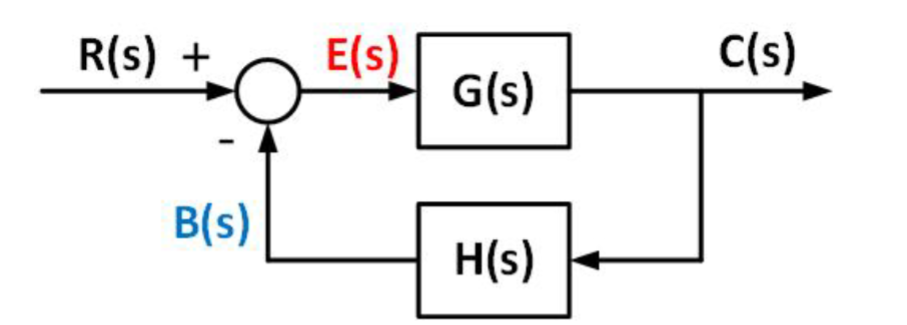
\includegraphics[width=0.5\linewidth,height=\textheight,keepaspectratio]{chapters/images/feedback-block-diagram-from-notes.png}

}

\caption{\label{fig-feedback-diagram}Feedback System Block Diagram}

\end{figure}%

From the schematic, the relation between the output and input is
computed as:

\[
    \textcolor{blue}{C(s) = G(s)E(s)}\qcomma \qqtext{where} \textcolor{red}{E(s) = R(s) - B(s) = R(s) - C(s)H(s)}
\]

Simple algebraic manipulation gives:

\[
\begin{aligned}
    C(s) &= G(s)E(s) \\
    &= G(s)[R(s) - C(s)H(s)] \\
    &= G(s)R(s) - G(s)C(s)H(s) \\
    \qor& C(s)[1 + G(s)H(s)] = G(s)R(s) \\
    \text{Therefore} & \qcomma \dfrac{C(s)}{R(s)} = \dfrac{G(s)}{1+G(s)H(s)} 
\end{aligned}
\]

Using this basic relationship of the feedback system structure, we can
uncover some of the significant effects of feedback.

\subsection{Effects of Feedback on System
Gain}\label{effects-of-feedback-on-system-gain}

We can relate the input and output of a system \emph{without} feedback
as:

\[
    C(s) = G(s)R(s) \qqtext{or,} \dfrac{C(s)}{R(s)} = G(s)
\]

As computed previously, based on the schematic of a feedback system, the
input-output relation is:

\[
\begin{aligned}
    E(s) &= R(s) - B(s) = R(s) - C(s)H(s) \\
    C(s) &= G(s)E(s) = G(s)[R(s) - C(s)H(s)] \\
    \qqtext{or,} C(s) &= G(s)R(s) - G(s)C(s)H(s) \\
    \qqtext{or,} C(s)&[1+G(s)H(s)] = G(s)R(s) \\
    \qqtext{Therefore,} \dfrac{C(s)}{R(s)} &= \dfrac{G(s)}{1+G(s)H(s)}
\end{aligned}
\]

Thus, the feedback affects the gain of the open loop system by a factor
\(1+G(s)H(s)\).

\subsection{Effects of Feedback on
Noise}\label{effects-of-feedback-on-noise}

To know the effect of feedback on noise, let us compare the transfer
functions with and without feedback due to the noise signal alone.
Consider an open loop system with noise signal as shown below.

The output is expressed as:

\[
    C(s) = [G_a(s)R(s) + N(s)]G_b(s) = G_a(s)G_b(s)R(s) + G_b(s)N(s)
\]

The open loop transfer function due to noise alone can be obtained by
making \(R(s) = 0\) which gives:

\[
    \dfrac{C(s)}{N(s)} = G_b(s)
\]

Consider the closed loop system with noise signal as shown below.

The output is expressed as:

\[
    C(s) = [(R(s) - H(s)C(s))G_a(s) + N(s)]G_b(s) = [G_a(s)R(s) - G_a(s)H(s)C(s) + N(s)]G_b(s)
\]

Further simplification gives:

\[
\begin{aligned}
    C(s) + G_a(s)G_b(s)H(s)C(s) &= G_a(s)G_b(s)R(s) + G_b(s)N(s) \\
\qqtext{or,}  C(s)[1+G_a(s)G_b(s)H(s)] &= G_a(s)G_b(s)R(s) + G_b(s)N(s)
\end{aligned}
\]

Thus

\[
    \textcolor{red}{C(s) = \dfrac{G_a(s)G_b(s)}{1+G_a(s)G_b(s)H(s)}R(s) + \dfrac{G_b(s)}{1+G_a(s)G_b(s)H(s)}N(s)}
\]

The closed loop transfer function due to noise alone can be obtained by
making \(R(s) = 0\) which gives:

\[
    \dfrac{C(s)}{N(s)} = \dfrac{G_b(s)}{1+G_a(s)G_b(s)H(s)} N(s)
\]

This shows that in the closed loop control system, the gain due to the
noise signal is decreased by a factor of \(1+G_a(s)G_b(s)H(s)\). Note
that, in most practical control systems, \((1+G_a(s)G_b(s)H(s))\) is
greater than 1.

\subsection{Effects of Feedback on Speed of
Response}\label{effects-of-feedback-on-speed-of-response}

\subsubsection{Case 1: Open Loop System}\label{case-1-open-loop-system}

Consider an open loop system with

\[
    G(s) = \dfrac{C(s)}{R(s)} = \dfrac{K}{s+a}
\]

The impulse response of this system is given by

\[  
    \textcolor{blue}{c(t) = \mathcal{L}^{-1}\left[C(s)\right]} = \mathcal{L}^{-1}\left[\dfrac{K}{s+\textcolor{red}{a}}\right] = K\textcolor{red}{e^{-at}}
\]

The time constant of the system \(\tau\) or \(T\) associated with this
mode of response equals to \(\textcolor{red}{\dfrac{1}{a}}\).

\subsubsection{Case 2: Closed Loop
System}\label{case-2-closed-loop-system}

When the feedback loop is closed with unity feedback, then

\[
    \textcolor{blue}{G(s) = \dfrac{C(s)}{R(s)} = \dfrac{G(s)}{1+G(s)} = \dfrac{\dfrac{K}{s+a}}{1+\dfrac{K}{s+a}}} = \dfrac{K}{s+\textcolor{red}{(a+K)}}
\]

The impulse response of this system is given by

\[  
    \textcolor{blue}{c(t) = \mathcal{L}^{-1}\left[C(s)\right]} = \mathcal{L}^{-1}\left[\dfrac{K}{s+\textcolor{red}{a + K}}\right] = K\textcolor{red}{e^{-(a+K)t}}
\]

The time constant of the system \(\tau\) or \(T\) associated with this
mode of response equals to \(\textcolor{red}{\dfrac{1}{a+K}}\).

\subsection{Effects of Feedback on
Stability}\label{effects-of-feedback-on-stability}

Consider the basic feedback system.

The input output relation is given by:

\[
    \dfrac{C(s)}{R(s)} = \dfrac{G(s)}{1+G(s)H(s)}
\]

From this it is obvious that when \(G(s)H(s) = -1\), the output of the
system will be infinite for any finite input, and the system is said to
be unstable.

Thus, Feedback can cause a system that is originally stable to become
unstable.

We will demonstrate that feedback can stabilize an unstable system.

\begin{figure}[H]

\centering{

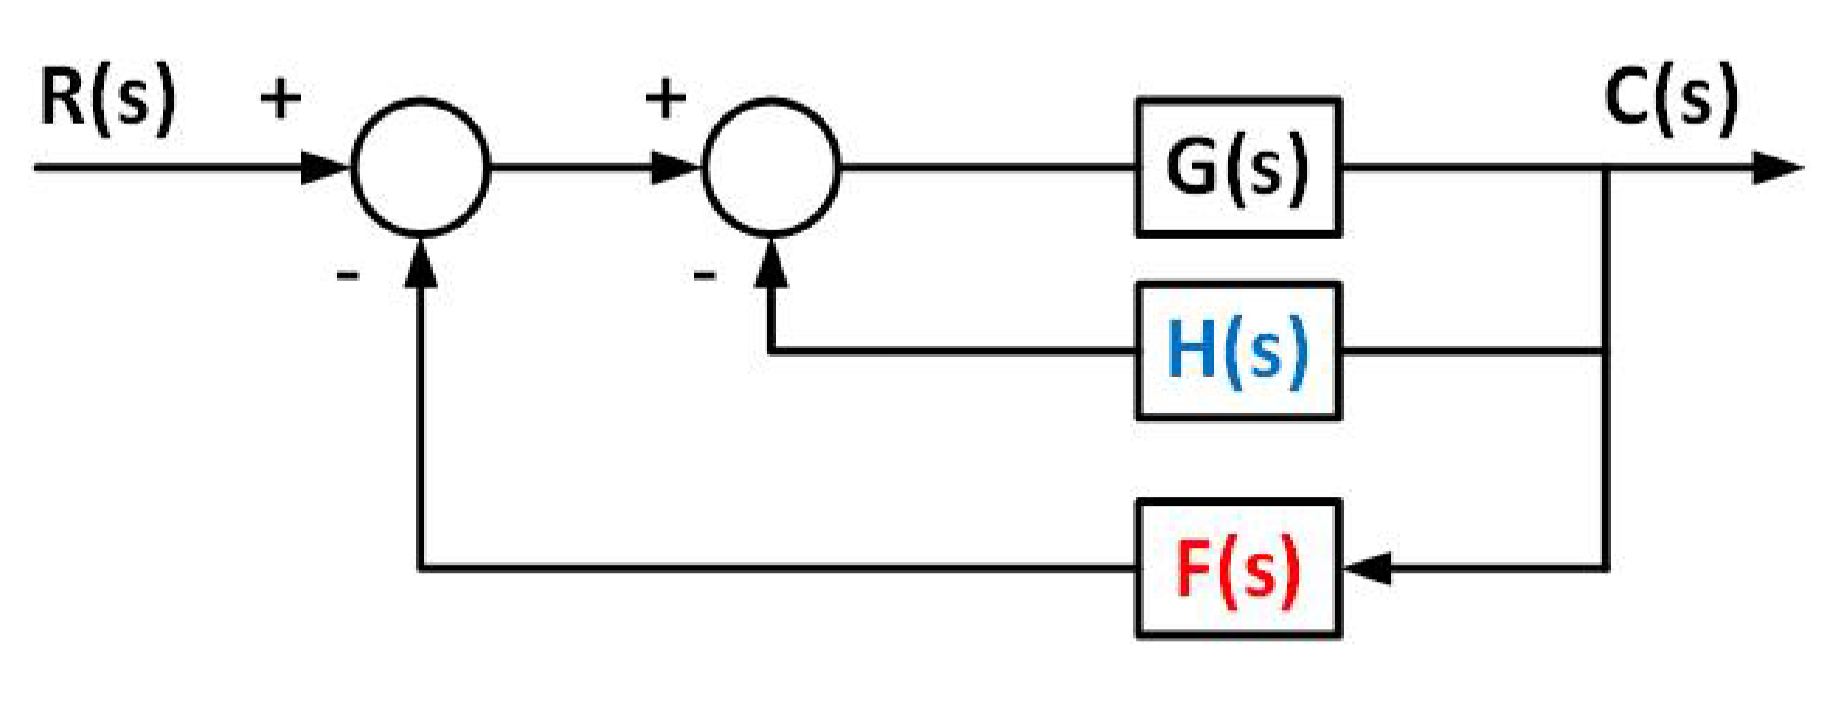
\includegraphics[width=0.5\linewidth,height=\textheight,keepaspectratio]{chapters/images/feedback-block-diagram-with-2-loop.png}

}

\caption{\label{fig-feedback-diagram-2}Two Loop Feedback System Block
Diagram}

\end{figure}%

Let us introduce another feedback loop through a negative feedback gain
\(F(s)\) as shown above. Then

\[
    \dfrac{C(s)}{R(s)} = \dfrac{G(s)}{1+G(s)H(s) + G(s)F(s)}
\]

The overall system can be made stable by properly selecting the outer
feedback gain \(F(s)\).

\subsection{Reduction of the Effects of Parameter
Variations}\label{reduction-of-the-effects-of-parameter-variations}

Let us define sensitivity on a quantitative basis. In the open loop case

\[
    C(s) = G(s)R(s)
\]

Suppose, due to parameter variations, \textcolor{red}{\(G(s)\) changes
to \([G(s) + \Delta G(s)]\)}.

The output of the open-loop system therefore changes to

\[
    C(s) + \Delta C(s) = [G(s) + \Delta G(s)]R(s)\qcomma \qqtext{Thus} \textcolor{red}{\Delta C(s) = \Delta G(s)R(s)}
\]

Similarly in the closed loop case, the output is given by

\[
    C(s) = \dfrac{G(s)}{1+G(s)H(s)}R(s)
\]

Due to variation \(\Delta G(s)\) in the forward path transfer function,
this changes to \[
    \textcolor{blue}{C(s) + \Delta C(s) = \dfrac{G(s) + \Delta G(s)}{1+[G(s) + \Delta G(s)]H(s)}R(s) = \dfrac{G(s) + \Delta G(s)}{1+G(s)H(s)+\Delta G(s)H(s)}R(s)}
\]

Since \(\abs{G(s)} \gg \abs{\Delta G(s)}\), the variation in the output
can be expressed as:

\[
    \textcolor{red}{\Delta C(s) = \dfrac{\Delta G(s)}{1+G(s)H(s)}R(s)}
\]

\begin{enumerate}
\def\labelenumi{\arabic{enumi}.}
\item
  \textcolor{blue}{\textbf{Open Loop System}} \[
   \textcolor{red}{\Delta C(s) = \Delta G(s)R(s)}
  \]
\item
  \textcolor{blue}{\textbf{Closed Loop System}}
\end{enumerate}

\[
    \textcolor{red}{\Delta C(s) = \dfrac{\Delta G(s)}{1+G(s)H(s)}R(s)}
\]

Thus, compared to the open loop system, the change in the output of the
closed loop system due to variations in \(G(s)\) is
\textcolor{red}{reduced by a factor of \([1+G(s)H(s)]\)} which often
much greater than unity or 1.

\subsection{Sensitivity Reduction Due to
Feedback}\label{sensitivity-reduction-due-to-feedback}

The term \textcolor{red}{\emph{system sensitivity}} is used to describe
the relative variation in the overall transfer function
\(T(s) = \dfrac{C(s)}{R(s)}\) due to variation in \(G(s)\) and is
defined as:

\[
    \textcolor{red}{\text{Sensitivity}} = \dfrac{\textcolor{blue}{\text{Percentage change in }T(s)}}{\textcolor{blue}{\text{Percentage change in }G(s)}}
\]

For a small incremental variation in \(G(s)\), the sensitivity of \(T\)
with respect to \(G\) is expressed quantitatively as:

\[
    \textcolor{red}{S^{T(s)}_{G(s)} = \pdv{T(s)/T(s)}{G(s)/G(s)} = \pdv{\ln{T(s)}}{\ln{G(s)}}}
\]

The sensitivity of the closed loop system is

\[
    \textcolor{blue}{S^{T(s)}_{G(s)} = \pdv{T(s)}{G(s)} \times \dfrac{G(s)}{T(s)} = \dfrac{(1+G(s)H(s))-G(s)H(s)}{(1+G(s)H(s))^2} \times \dfrac{G(s)}{\dfrac{G(s)}{1+G(s)H(s)}} = \dfrac{1}{1+G(s)H(s)}}
\]

The sensitivity of the open loop system is

\[
    \textcolor{red}{S^{T(s)}_{G(s)} = \pdv{T(s)}{G(s)} \times \dfrac{G(s)}{T(s)} = 1 \qcomma (\because \text{Here } T(s) = G(s))}
\]

Thus due to variations in \(G(s)\), the sensitivity of the closed loop
system is reduced by a factor of \(1+G(s)H(s)\) compared to the open
loop system.

The sensitivity of \(T(s)\) with respect to the feedback sensor \(H(s)\)
is given as

\[
    \textcolor{red}{S^{T(s)}_{H(s)} = \pdv{T(s)}{H(s)} \times \dfrac{H(s)}{T(s)} = G(s)\left[\dfrac{-G(s)}{(1+G(s)H(s))^2} \right] \times \dfrac{H(s)}{\dfrac{G(s)}{1+G(s)H(s)}} = \dfrac{-G(s)H(s)}{1+G(s)H(s)}}
\]

This shows that for large values of \(G(s)H(s)\) the sensitivity of the
feedback system with respect to \(H\) is unity. This implies that
\textcolor{blue}{changes in \(H\) directly affect the system output}.
Therefore, it is \textcolor{red}{important to use feedback elements}
\textcolor{blue}{which remain substantially constant and do not vary
with environmental changes}.

Very often, we are interested to find the sensitivity of a system with
respect to variation in a particular parameter or set of parameters.

Let the transfer function of the system be expressed as

\[
    T(s) = \dfrac{N(s,\alpha)}{D(s,\alpha)}; \quad \alpha = \text{parameter under consideration}
\]

The sensitivity of \(T(s)\) with respect to the parameter \(\alpha\) is
given by

\[
    \textcolor{red}{S^{T(s)}_{\alpha} = \pdv{\ln{N(s)}}{\ln{\alpha}}\Bigg|_{\alpha_0} - \pdv{\ln{D(s)}}{\ln{\alpha}}\Bigg|_{\alpha_0} = S^{N(s)}_{\alpha} - S^{D(s)}_{\alpha}}
\]

where \(\alpha_0\) is the nominal value of the parameter around which
variation occurs.

To have a highly accurate open-loop system, the components of \(G(s)\)
must be selected to rigidly meet the specifications. However, in a
closed loop system, \textcolor{blue}{\(G(s)\) may be less rigidly
specified,} \textcolor{red}{since the effects of parameter variations
can be mitigated by use of feedback}. Furthermore, however, a closed
loop system requires \textcolor{blue}{careful selection of components of
the feedback sensor \(H(s)\)}. Note that \(H(s)\) is often made up of
measuring elements which operate at lower power levels and are less
costly.

\subsection{Effect of High Gain in a Feedback
System}\label{effect-of-high-gain-in-a-feedback-system}

It will be shown that using high gain in a feedback system can make the
output track the input.

Consider a system with \textcolor{red}{gain \(K\)}.

The closed loop output (\(C(s)\)) and the error (\(E(s)\)) response can
be expressed as:

\[
    C(s) = \dfrac{KG(s)}{1+KG(s)}R(s) \qcomma E(s) = \dfrac{1}{1+KG(s)}R(s)
\]

From these, it is obvious that as \(K \to \infty\), \(C(s) \to R(s)\)
and \(\textcolor{red}{E(s) \to 0}\).

\begin{itemize}
\item
  Open Loop Gain: \(\textcolor{blue}{\abs{KG(s)}\gg 1}\)
\item
  Closed Loop Gain:
  \(\textcolor{red}{\abs{\dfrac{KG(s)}{1+KG(s)}}\approx 1}\)
\end{itemize}

Thus we can make \textcolor{red}{the output track the input} even if
\textcolor{blue}{we do not know the exact value of the open loop gain}.

\section{Advantages and Disadvantages of Closed Loop
Control}\label{advantages-and-disadvantages-of-closed-loop-control}

\begin{figure}[h!]

\begin{minipage}{0.47\linewidth}
\textcolor{red}{\textbf{Advantages of a Closed Loop Control System:}}

\begin{enumerate}
\def\labelenumi{\arabic{enumi}.}
\tightlist
\item
  \textcolor{red}{More accurate even in the presence of non-linearity}.
\item
  Highly accurate as any error is corrected due to the presence of the
  feedback signal.
\item
  \textcolor{blue}{Bandwidth range is large}.
\item
  Facilitates automation.
\item
  The sensitivity of the system may be made small to make the system
  more stable.
\item
  The system is \textcolor{red}{less affected by noise.}
\end{enumerate}

\end{minipage}%
%
\begin{minipage}{0.05\linewidth}
~\end{minipage}%
%
\begin{minipage}{0.47\linewidth}
\textcolor{red}{\textbf{Disadvantages of a Closed Loop Control System:}}

\begin{enumerate}
\def\labelenumi{\arabic{enumi}.}
\tightlist
\item
  Costly to implement
\item
  Complexity is increased.
\item
  More maintenance is required.
\item
  Feedback can lead to oscillations.
\item
  Feedback reduces overall gain.
\item
  \textcolor{red}{Stability is the most major problem} and more care is
  needed to design a stable closed loop system.
\end{enumerate}

\end{minipage}%
%
\begin{minipage}{0.01\linewidth}
~\end{minipage}%

\end{figure}%

\subsection{Comparison Between Open Loop and Closed Loop
Control}\label{comparison-between-open-loop-and-closed-loop-control}

\begin{figure}[H]

\begin{minipage}{0.50\linewidth}
\textcolor{red}{\textbf{Open Loop Control}}

\begin{enumerate}
\def\labelenumi{\arabic{enumi}.}
\tightlist
\item
  The feedback element is absent.
\item
  An error detector is not present.
\item
  Easy to construct.
\item
  Have small bandwidth
\item
  Often Stable.
\item
  Less maintenance.
\item
  Often unreliable.
\end{enumerate}

\end{minipage}%
%
\begin{minipage}{0.50\linewidth}
\textcolor{red}{\textbf{Closed Loop Control}}

\begin{enumerate}
\def\labelenumi{\arabic{enumi}.}
\tightlist
\item
  The feedback element is present.
\item
  An error detector is always present.
\item
  Complicated construction.
\item
  Have large bandwidth.
\item
  May become unstable.
\item
  More maintenance.
\item
  Reliable.
\end{enumerate}

\end{minipage}%

\end{figure}%

\section{Summary of Important Characteristics of a Feedback
System}\label{summary-of-important-characteristics-of-a-feedback-system}

\begin{enumerate}
\def\labelenumi{\arabic{enumi}.}
\item
  \textcolor{red}{Decreased Sensitivity} of the system to variations in
  the process parameters.
\item
  Improved \textcolor{red}{rejection of disturbances}.
\item
  Improved \textcolor{red}{measurement noise attenuation}.
\item
  Improved \textcolor{red}{reduction in steady state error} of the
  system.
\item
  Easy \textcolor{red}{control and adjustment of the transient response}
  of the system.
\end{enumerate}

\chapter{Time Domain Analysis of Linear Systems: Time Domain
Specifications}\label{time-domain-analysis-of-linear-systems-time-domain-specifications}

\section*{Learning Outcomes}\label{learning-outcomes-3}
\addcontentsline{toc}{section}{Learning Outcomes}

\markright{Learning Outcomes}

After completing this module, you should be able to:

\begin{enumerate}
\def\labelenumi{\arabic{enumi}.}
\item
  Understand the concepts of Transient and Steady-State Responses.
\item
  Know the Typical input signals used for time domain analysis.
\item
  Compute various time domain specifications such as rise time, peak
  time, peak overshoot etc. for an underdamped second order control
  system.
\end{enumerate}

\section{Transient and Steady-State
Response}\label{transient-and-steady-state-response}

It is to be of note that: Systems with energy storage elements
(i.e.~dynamic systems) can not respond instantaneously and will exhibit
transient responses whenever they are subjected to inputs or
disturbances.

The time response \(c(t)\) of a control system is usually divided into
two parts: \textcolor{red}{the transient response} and
\textcolor{red}{the steady-state response}.

Thus, the total response is given by:

\[
    \textcolor{blue}{c(t) = c_{tr}(t) + c_{ss}(t)}
\]

where \(c_{tr}(t)\) is the transient response and \(c_{ss}(t)\) is the
steady-state response.

Transient response is defined as the part of the response that goes to
zero as time ``becomes large'' or rather goes to infinity. Therefore,
\(c_{tr}(t)\) has the property of

\[
    \textcolor{red}{\lim\limits_{t \to \infty} c_{tr}(t) = 0}
\]

The definition of the steady state, however, has not been entirely
standardized. In circuit analysis/theory, it is sometimes useful to
define a steady-state variable as being a constant with respect to time.

In control systems, however, the steady-state response is simply the
fixed response when time reaches infinity. When a response reaches
steady state, it can still vary with time.

For example, a sine wave is considered as a steady-state response
because its behavior is fixed for any time interval, as when time
approaches infinity. Similarly, if a response is described by
\(c(t) = t\), it may be defined as a steady-state response.

\section{Test Signals for Time Domain
Analysis}\label{test-signals-for-time-domain-analysis}

\subsection{\texorpdfstring{\textcolor{red}{Why is there a need for Test
Signals?}}{Why is there a need for Test Signals?}}\label{why-is-there-a-need-for-test-signals}

The input excitation to many practical control systems are not known
ahead of time; unlike many electrical circuits and communication
systems.

In many cases, the actual inputs of a control system may vary in random
fashions with respect to time.

\begin{itemize}
\tightlist
\item
  For instance, in a radar tracking system, the position and speed of
  the target to be tracked may vary in an unpredictable manner, so that
  they cannot be expressed deterministically by a mathematical
  expression.
\end{itemize}

This is a major problem for designers, since it is difficult to design
the control system so that it will perform satisfactorily to any
possible input signal.

\textcolor{red}{For the purposes of analysis and design, it is necessary
to assume some basic types of input functions so that the performance of
a system can be evaluated with respect to these test signals.}

By selecting these basic test signals properly, not only the
mathematical treatment of the problem is systemized, but the responses
due to these inputs allow the prediction of the system's performance to
other more complex inputs.

In a design problem, performance criteria may be specified with respect
to these test signals so that a system may be designed to meet these
criteria.

The general form of the signals used for time domain analysis can be
expressed as:

\[
    \textcolor{blue}{r(t) = At^n; \quad R(s) = \dfrac{n!A}{s^{n+1}}}
\]

When \(n=0\), this corresponds to a step signal, when \(n=1\), this
represents a ramp signal, and when \(n=2\), this corresponds a parabolic
signal.

It is to be of note, however, that from the step function to the
parabolic function, the signals become progressively faster with respect
to time.

\begin{enumerate}
\def\labelenumi{\arabic{enumi}.}
\item
  The step function is very useful as a test signal, since its initial
  instantaneous jump in amplitude reveals a great deal about a system's
  quickness to respond.
\item
  The ramp function has the ability to test how the system would respond
  to a signal that changes linearly with time.
\item
  The parabolic function is one degree faster than the ramp function. In
  practice, we seldom find it necessary to use a test signal faster than
  a parabolic function.
\end{enumerate}

\subsection{\texorpdfstring{\textcolor{red}{Step
Input}}{Step Input}}\label{step-input}

Frequently the performance characteristics of a control system are
specified in terms of transient response to a unit-step input. This is
because:

\begin{enumerate}
\def\labelenumi{\arabic{enumi}.}
\item
  They are easy to generate.
\item
  Its initial instantaneous jump in amplitude reveals a great deal about
  a system's quickness to respond
\item
  Also, since the step function has, in principle, a wide band of
  frequencies in its spectrum, as a result of the jump discontinuity, as
  a test signal it is equivalent to the application of numerous
  sinusoidal signals with a wide range of frequencies.
\end{enumerate}

\subsection{\texorpdfstring{\textcolor{red}{Ramp
Input}}{Ramp Input}}\label{ramp-input}

The ramp function is a signal that changes constantly with respect to
time.

Mathematically, a ramp function is represented by

\[
    \textcolor{blue}{r(t) = At}
\]

where \(A\) is a real constant.

The ramp function has the ability to test how the system would respond
to a signal that changes linearly with time.

\subsection{\texorpdfstring{\textcolor{red}{Parabolic
Input}}{Parabolic Input}}\label{parabolic-input}

The parabolic function represents a signal that is one order faster than
the ramp function.

Mathematically, a parabolic function is represented by

\[
    \textcolor{blue}{r(t) = \dfrac{At^2}{2}}
\]

where \(A\) is a real constant. Note that the factor of \(\dfrac{1}{2}\)
is added for mathematical convenience; because the Laplace transform of
\(r(t)\) becomes \(\dfrac{A}{s^3}\).

Note: From the step function to the parabolic function, the signals
become progressively faster with respect to time.

\section{Time Domain Analysis of First Order
System}\label{time-domain-analysis-of-first-order-system}

Consider a first order system without a zero shown in Figure 1

This is a generic first order system, and may represent an R-L circuit,
R-C circuit, a simple thermal system and so on. The relationship between
the input and output is given by

\begin{equation}\phantomsection\label{eq-generic-first-order-system}{
    \dfrac{C(s)}{R(s)} = \dfrac{1}{Ts+1}
}\end{equation}

Eqn(Equation~\ref{eq-generic-first-order-system}) can alternately be
expressed as:

\begin{equation}\phantomsection\label{eq-reexpressed-first-order-system}{
    \dfrac{C(s)}{R(s)} = \dfrac{1/T}{s+1/T} = \dfrac{a}{s+a} \qcomma \qqtext{where} a = \dfrac{1}{T}
}\end{equation}

The block diagram, corresponding to the system in
Eqn(Equation~\ref{eq-reexpressed-first-order-system}), is shown in
Figure 2a and the pole location is shown in the s-plane in Figure 2b.

The step response of this system, i.e.~when \(R(s) = \dfrac{1}{s}\), is
given by

\[
    C(s) = G(s)R(s) = \dfrac{a}{s(s+a)} = \dfrac{1}{s} - \dfrac{1}{s+a}
\]

Which in the time domain gives us:

\[
    c(t) = c_f(t) + c_n(t) = 1 - e^{-at}
\]

The step response of the first order system is shown in the Figure.

\subsection{\texorpdfstring{\textcolor{red}{Time Constant \(T\) (or
\(\tau\))}}{Time Constant T (or \textbackslash tau)}}\label{time-constant-t-or-tau}

The time constant is defined as the time required for the step response
to reach \(63\%\) of its final value. It is denoted by \(T\) or
\(\tau\).

\subsection{Computation of Time Constant for a First Order
System}\label{computation-of-time-constant-for-a-first-order-system}

We Know that the step response of a first order system is given by

\[
    \textcolor{blue}{c(t) = 1 - e^{-at}}
\]

Let \(T\) be the time when the response equals to 0.63.
i.e.~\(c(T) = 0.63\). This implies

\[
    1 - e^{-aT} = 0.63 \implies aT = \ln\left({\dfrac{1}{0.37}}\right) = \ln(2.7027) \approx 1 \implies T \approx \dfrac{1}{a}
\]

Thus the time constant \(T\) equals to

\[
    \textcolor{red}{T = \dfrac{1}{a}}
\]

\subsection{\texorpdfstring{\textcolor{red}{Rise Time
\(T_r\)}}{Rise Time T\_r}}\label{rise-time-t_r}

The rise time is defined as the time required for the response to go
from \(10\%\) (0.1) to \(90\%\) (0.9) of its final value. It is denoted
by \(T_r\).

\subsection{Computation of Rise Time for a First Order
System}\label{computation-of-rise-time-for-a-first-order-system}

We Know that the step response of a first order system is given by

\[
    \textcolor{blue}{c(t) = 1 - e^{-at}}
\]

Let \(t_0\) be the time when the response equals to 0.1.
i.e.~\(c(t_0) = 0.1\). This implies

\[
    1 - e^{-at_0} = 0.1 \implies at_0 = \ln\left({\dfrac{10}{9}}\right) \approx 0.11 \implies t_0 \approx \dfrac{0.11}{a}
\]

Let \(t_1\) be the time when the response equals to 0.9.
i.e.~\(c(t_1) = 0.9\). This implies

\[
    1 - e^{-at_1} = 0.9 \implies at_1 = \ln(10) \approx 2.31 \implies t_1 \approx \dfrac{2.31}{a}
\]

Thus the \textcolor{blue}{\textbf{rise time} \(T_r\)} equals to

\[
    \textcolor{red}{T_r = t_1 - t_0 \approx \dfrac{2.31}{a}-\dfrac{0.11}{a} = \dfrac{2.2}{a}}
\]

\subsection{\texorpdfstring{\textcolor{red}{Settling Time
\(T_s\)}}{Settling Time T\_s}}\label{settling-time-t_s}

The settling time is defined as the time required for the response to
reach and stay within, in our case, \(2\%\) of its final value. It is
denoted by \(T_s\).

\subsection{Computation of Settling Time for a First Order
System}\label{computation-of-settling-time-for-a-first-order-system}

We Know that the step response of a first order system is given by

\[
    \textcolor{blue}{c(t) = 1 - e^{-at}}
\]

Let \(T_s\) be the time when the response equals to 0.98.
i.e.~\(c(T_s) = 0.98\). This implies

\[
    1 - e^{-aT_s} = 0.98 \implies aT_s = \ln(50) \approx 3.91 \implies T_s \approx \dfrac{3.91}{a}
\]

Thus the \textcolor{blue}{\textbf{settling time} \(T_s\)} equals to

\[
    \textcolor{red}{T_s = \dfrac{3.91}{a} \approx \dfrac{4}{a}}
\]

\section{DC Gain of a System}\label{dc-gain-of-a-system}

This is the gain of the system when the input frequency is zero.
Therefore it is also know as zero frequency gain of the system. It is
the ratio of the magnitude of the steady state output to that of the
constant input, provided the output is finite. This can be computed as
follows:

Consider the system with the transfer function

\[
    G(s) = \dfrac{C(s)}{R(s)} 
\]

If we apply a unity step input \(R(s) = \dfrac{1}{s}\), the steady state
value of the output becomes

\begin{equation}\phantomsection\label{eq-dc-gain}{
    \lim\limits_{t \to \infty} c(t) = \lim\limits_{s \to 0} sG(s)R(s) = \lim\limits_{s \to 0} sG(s)\dfrac{1}{s} = \lim\limits_{s \to 0} G(s)
}\end{equation}

Since the input is a constant of magnitude unity (1), the steady state
output is also the gain in the steady state; that is \(G(0)\). Thus

\begin{equation}\phantomsection\label{eq-dc-gain-from-ss}{
    \textcolor{red}{\mathrm{DC\ Gain} = \lim\limits_{s \to 0} G(s) = G(0)}
}\end{equation}

\section{Time Domain Analysis of Second Order
System}\label{time-domain-analysis-of-second-order-system}

Consider a second order system shown in the Figure

The closed loop transfer function of this system is given by

\[
    \textcolor{blue}{\dfrac{C(s)}{R(s)}=\dfrac{\omega_n^2}{s^2 + 2\zeta\omega_ns + \omega_n^2}}
\]

(The notes used \(\xi\), incorrectly, but was always read as \(\zeta\),
which is the correct symbol used according to wikipedia)

The parameter \(\textcolor{red}{\omega_n}\) is the
\textcolor{red}{natural frequency} of the second order system, and the
parameter \(\textcolor{red}{\zeta}\) is called the
\textcolor{red}{damping ratio}.

The closed loop poles \(\lambda_{1,2}\) are given by

\[
    \textcolor{red}{\lambda_{1,2} = -\zeta \omega_n \pm \omega_n \sqrt{\zeta^2 - 1}}
\]

The nature of the response of the system depends on the value of the
damping ratio \(\zeta\). The following discusses the step responses of
this system for different cases.

\subsection{\texorpdfstring{\textcolor{blue}{Case 1:
\(\zeta = 0\)}}{Case 1: \textbackslash zeta = 0}}\label{case-1-zeta-0}

\begin{itemize}
\item
  The closed loop poles are located at \(\pm j\omega_n\).
\item
  The step response under this case will be sinusoidal with frequency
  \(\omega_n\) and is expressed as:
\end{itemize}

\[
    c(t)=1-\cos(\omega_n t)
\]

\begin{itemize}
\tightlist
\item
  This type of response is called an \textcolor{red}{\textbf{undamped}}
  response.
\end{itemize}

\subsection{\texorpdfstring{\textcolor{blue}{Case 2:
\(0 < \zeta < 1\)}}{Case 2: 0 \textless{} \textbackslash zeta \textless{} 1}}\label{case-2-0-zeta-1}

\begin{itemize}
\item
  The closed loop poles are located at
  \(-\zeta \omega_n \pm j\omega_n\sqrt{1-\zeta^2}\).
\item
  The step response is a damped sinusoid with an exponential envelope
  whose time constant is equal to the reciprocal of the real part of the
  poles. It is expressed as:
\end{itemize}

\[
\begin{aligned}
    c(t) &= 1 - \dfrac{1}{\sqrt{1-\zeta^2}}e^{-\zeta\omega_n t} \cos(\omega_d t + \phi); \qqtext{where} \\
    \omega_d &= \omega_n \sqrt{1-\zeta^2}; \quad \phi = \tan^{-1}\left(\dfrac{\zeta}{\sqrt{1-\zeta^2}}\right)
\end{aligned}
\]

\begin{itemize}
\tightlist
\item
  This type of response is called an \textcolor{red}{\textbf{under
  damped}} response.
\end{itemize}

\subsection{\texorpdfstring{\textcolor{blue}{Case 3:
\(\zeta = 1\)}}{Case 3: \textbackslash zeta = 1}}\label{case-3-zeta-1}

\begin{itemize}
\item
  We have two closed loop poles which are real
  (i.e.~\(\lambda \in \mathbb{R}\)) and are located at
  \(-\zeta \omega_n\).
\item
  The step response under this case will be expressed as:
\end{itemize}

\[
\begin{aligned}
    c(t) &= 1 - \zeta \omega_n t e^{-\zeta \omega_n t} - e^{-\zeta \omega_n t} \\
    &= 1 - e^{-\zeta \omega_n t}(1+\zeta\omega_n t)
\end{aligned}
\]

\begin{itemize}
\tightlist
\item
  This type of response is called a \textcolor{red}{\textbf{critically
  damped}} response.
\end{itemize}

\subsection{\texorpdfstring{\textcolor{blue}{Case 4:
\(\zeta > 1\)}}{Case 4: \textbackslash zeta \textgreater{} 1}}\label{case-4-zeta-1}

\begin{itemize}
\item
  The two closed loop poles are real (i.e.~\(\lambda \in \mathbb{R}\))
  and are located at \(-\zeta\omega_n \pm \omega_n \sqrt{\zeta^2 - 1}\)
\item
  The step response under this case will be expressed as:
\end{itemize}

\[
    c(t)= 1- e^{-(\zeta-\sqrt{\zeta^2-1})\omega_n t}
\]

\begin{itemize}
\tightlist
\item
  This type of response is called an \textcolor{red}{\textbf{over
  damped}} response.
\end{itemize}

\section{Transient (Time) Response Specifications: Some
Notes}\label{transient-time-response-specifications-some-notes}

Control systems are generally designed with damping less than one,
i.e.~oscillatory step response.

Higher-order control systems usually have a pair of complex conjugate
poles with damping less than one which dominate over the other poles
\textcolor{red}{\textbf{(dominant pole pairs)}}.

Thus the time response of second and higher-order control systems to a
step input, is in general, of a \textcolor{red}{\textbf{damped
oscillatory nature}}.

It is observed that the step response has a number of
\textcolor{red}{\textbf{overshoots}} and
\textcolor{red}{\textbf{undershoots}} with respect to the final steady
state value.

This type of response is expressed mathematically as:

\[
    \textcolor{blue}{c(t) = 1 - \dfrac{e^{-\zeta \omega_n t}}{\sqrt{1-\zeta^2}} \cos{(\omega_d t + \phi)}\qcomma} \qqtext{where} \textcolor{red}{\omega_d = \omega_n \sqrt{1-\zeta^2} \qcomma \phi = \tan^{-1}\left(\dfrac{\zeta}{\sqrt{1-\zeta^2}}\right)}
\]

The pole plot of the \textcolor{red}{\textbf{underdamped}} second order
system is shown in the figure

This type of response is characterised by the following performance
indicies:

\begin{enumerate}
\def\labelenumi{\arabic{enumi}.}
\item
  \textcolor{red}{Rise Time \(T_r\)}
\item
  \textcolor{blue}{Peak Time \(T_p\)}
\item
  \textcolor{red}{Peak Overshoot \(M_p\)}
\item
  \textcolor{blue}{Settling Time \(T_s\)}
\item
  \textcolor{red}{Steady State Error \(e_{ss}\)}
\end{enumerate}

These indicies are qualitatively related to

\begin{enumerate}
\def\labelenumi{\alph{enumi}.}
\item
  \textcolor{red}{How fast is the system? i.e.~how fast it moves to
  follow the input?}
\item
  \textcolor{blue}{How oscillatory the system is? (indicative of
  damping)}
\item
  \textcolor{red}{How long does it take to practically reach the final
  value?}
\end{enumerate}

\textcolor{red}{\textbf{Note:}} \textcolor{blue}{The various indicies
are not independent of each other.}

\section{Commonly Used Transient Response
Specification}\label{commonly-used-transient-response-specification}

\subsection{\texorpdfstring{\textcolor{red}{Rise Time
\(T_r\)}}{Rise Time T\_r}}\label{rise-time-t_r-1}

\begin{itemize}
\item
  It is the time required for the response to rise from \(10\%\) to
  \(90\%\), \(5\%\) to \(95\%\), or \(0\%\) to \(100\%\) of its final
  value.
\item
  For underdamped, second-order systems, the \(0\%\) to \(100\%\) rise
  time is normally used. For overdamped systems, the \(10\%\) to
  \(90\%\) rise time is commonly used.
\item
  Analytically, it is expressed as
\end{itemize}

\[
    \textcolor{red}{T_r = \dfrac{1}{\omega_d} \tan^{-1}\left(\dfrac{\omega_d}{-\sigma_d} \right) = \dfrac{\pi - \theta}{\omega_d}}
\]

\subsection{\texorpdfstring{\textcolor{red}{Peak Time
\(T_p\)}}{Peak Time T\_p}}\label{peak-time-t_p}

\begin{itemize}
\item
  It is the time required for the response to reach the first peak of
  the overshoot.
\item
  Analytically, it is expressed as
\end{itemize}

\[
    \textcolor{red}{T_p = \dfrac{\pi}{\omega_n \sqrt{1-\zeta^2}} = \dfrac{\pi}{\omega_d}}
\]

\subsection{\texorpdfstring{\textcolor{red}{Maximum (percent) Overshoot
\(\%OS\), or
\(M_p\)}}{Maximum (percent) Overshoot \textbackslash\%OS, or M\_p}}\label{maximum-percent-overshoot-os-or-m_p}

\begin{itemize}
\tightlist
\item
  It is the maximum peak value of the response. It is defined by
\end{itemize}

\[
    \textcolor{blue}{M_p = \dfrac{c(t_p)-c(\infty)}{c(\infty)} \times 100\%}
\]

\begin{itemize}
\tightlist
\item
  Analytically, it is expressed as
\end{itemize}

\[
    \textcolor{red}{\%OS = e^{-\left(\dfrac{\pi\zeta}{\sqrt{1-\zeta^2}}\right)}}
\]

\subsection{\texorpdfstring{\textcolor{red}{Settling Time
\(T_s\)}}{Settling Time T\_s}}\label{settling-time-t_s-1}

\begin{itemize}
\tightlist
\item
  It is teh time required for the response to reach and stay within
  either \(2\%\) or \(5\%\) of its final (steady-state) value. Commonly
  it is expressed as:
\end{itemize}

\[
    \textcolor{red}{T_s = 4T = \dfrac{4}{\sigma_d} = \dfrac{4}{\zeta \omega_n} \quad \text{(2\% criterion)}} 
\]

\[
    \textcolor{red}{T_s = 3T = \dfrac{3}{\sigma_d} = \dfrac{3}{\zeta \omega_n} \quad \text{(5\% criterion)}}
\]

\section{Correlation Between Pole Locations with Time Domain
Specifications}\label{correlation-between-pole-locations-with-time-domain-specifications}

\begin{enumerate}
\def\labelenumi{\arabic{enumi}.}
\item
  The radial distance from the origin to the pole is the natural
  frequency \(\omega_n\).
\item
  The damping ratio \(\zeta\) is equal to \(\cos(\theta)\),
  i.e.~\(\cos(\theta) = \zeta\).
\item
  We know that the peak time and settling time are
\end{enumerate}

\[
    \textcolor{red}{T_p = \dfrac{\pi}{\omega_n \sqrt{1-\zeta^2}} = \dfrac{\pi}{\omega_d} \qquad T_s = \dfrac{4}{\zeta\omega_n} = \dfrac{4}{\sigma_d}}
\]

where \(\omega_d\) is the imaginary part of the pole and is called the
damped frequency of oscillation, and \(\sigma_d\) is the magnitude of
the real part of the pole and is the exponential damping frequency.

\begin{enumerate}
\def\labelenumi{\arabic{enumi}.}
\setcounter{enumi}{3}
\item
  Thus \textcolor{red}{\(T_p\) is inversely proportional to the
  imaginary part of the pole}.
\item
  \textcolor{blue}{\(T_s\) is inversely proportional to the real part of
  the pole}.
\end{enumerate}

\section{Examples: Time Domain
Specifications}\label{examples-time-domain-specifications}

\section{\texorpdfstring{Effects of Changing Exponential Damping
Frequency \(\omega_d\) \& Damped Frequency \(\sigma_d\) on Time
Response}{Effects of Changing Exponential Damping Frequency \textbackslash omega\_d \& Damped Frequency \textbackslash sigma\_d on Time Response}}\label{effects-of-changing-exponential-damping-frequency-omega_d-damped-frequency-sigma_d-on-time-response}

\begin{itemize}
\tightlist
\item
  The poles are located at
  \(\textcolor{blue}{-\sigma_d \pm j\omega_d}\). The peak time \(T_p\)
  and settling time \(T_s\) are
\end{itemize}

\[
    \textcolor{red}{T_p = \dfrac{\pi}{\omega_d}, \qand T_s = \dfrac{4}{\sigma_d}}
\]

\begin{enumerate}
\def\labelenumi{\arabic{enumi}.}
\item
  Vary \(\omega_d\) and fix \(\sigma_d\). The frequency of oscillation
  and the peak time change; but the settling time remains unchanged.
\item
  Vary \(\sigma_d\) and fix \(\omega_d\). The frequency of oscillation
  and the peak time remain unchanged; but the settling time changes.
\item
  Vary the natural frequency \(\omega_n\) and fix \(\zeta\). The
  percentage overshoot remains unchanged; but the settling time changes.
\item
  Thus \(T_p\) is inversely proportional to the imaginary part of the
  pole.
\item
  \(T_s\) is inversely proportional to the real part of the pole.
\end{enumerate}

\chapter{Stability Analysis of Linear Systems: Routh-Hurwitz Stability
Criteria}\label{stability-analysis-of-linear-systems-routh-hurwitz-stability-criteria}

\section*{Learning Outcomes}\label{learning-outcomes-4}
\addcontentsline{toc}{section}{Learning Outcomes}

\markright{Learning Outcomes}

After completing this module, you should be able to:

\begin{enumerate}
\def\labelenumi{\arabic{enumi}.}
\item
  Determine the absolute stability of a linear system.
\item
  Find the stability region of a linear system.
\end{enumerate}

\section{Concept of Stability}\label{concept-of-stability}

A system is stable if small changes in system inputs, initial
conditions, or system parameters do not result in large changes in
system behaviour. Intuitively, a system is stable if it remains at rest
unless excited by an external source and returns to rest if all
excitations are removed.

\textcolor{blue}{\textbf{Absolute Stability}}

Suppose the ball is initially inside the bowl in position 1. If it is
perturbed from its inital position by a small force, it will cause the
ball to move. When the force is removed, the ball will oscillate and
eventually return to its initial position. This is an example of
\textcolor{red}{\textbf{absolutely stable dynamics}}.

\textcolor{blue}{\textbf{Instability}}

Consider the situation where the bowl is turned upside down and the ball
is placed on the top of the bowl. When the ball is slightly perturbed by
the application of a force, it begins to move on its own without any
additional force applied. It will never return to its original position.
This is an example of \textcolor{red}{\textbf{unstable dynamics}}.

\textcolor{blue}{\textbf{Neutral Stability}}

If the ball is placed on a flat surface, then after the application of a
small force, the ball will move. but when the force is withdrawn, the
ball stops and remains in its new position. This is an example of
\textcolor{red}{\textbf{neutral stability}}.

Suppose a system has an equilibrium point at \(x = x_e\). In stability
studies we generally address the following questions:

\begin{enumerate}
\def\labelenumi{\arabic{enumi}.}
\tightlist
\item
  If the system with zero input is perturbed from its equilibrium point
  \(x_e\) at \(t = t_0\), will the state \(x(t)\)

  \begin{enumerate}
  \def\labelenumii{\alph{enumii}.}
  \tightlist
  \item
    Return to \(x_e\)?
  \item
    Remain close to \(x_e\)? or
  \item
    Diverge from \(x_e\)?
  \end{enumerate}
\item
  If the system is relaxed, will a \textbf{bounded input} produce
  \textbf{a bounded output}?
\end{enumerate}

Consider the ball which is free to roll on the surface.

The ball could be made to rest at points \textcolor{blue}{\textbf{A, E,
F, G}} and \textcolor{blue}{anywhere between the points \textbf{B and D,
such as C.}} An perturbation away from A or F will cause the ball to
diverge from these points. Thus \textcolor{red}{A and F are
\textbf{unstable equilibrium points}}. After small perturbations away
from E or G, the ball will eventually return to these points. Thus
\textcolor{red}{E and G are \textbf{stable equilibrium points}}. If the
ball is perturbed slightly away from C, it will remain at the new
position. \textcolor{red}{Points like C are sometimes said to be
\textbf{neutrally stable}}.

The following figure shows different types of possible stability
surfaces for globally stable, stable, unstable and locally stable
systems.

\subsection{Definitions of Stability, Instability and Marginal
Stability}\label{definitions-of-stability-instability-and-marginal-stability}

The total response of a system \(c(t)\) of a dynamic system is expressed
as:

\begin{equation}\phantomsection\label{eq-total-response}{
    c(t) = c_{\text{forced}}(t) + c_{\text{natural}}(t)
}\end{equation}

Based on the \textbf{natural response}, we define stability, instability
and marginal stability as follows:

\begin{description}
\item[Stable]
A linear time invariant system is stable provided its natural response
converges to zero as time approaches infinity.
\item[Unstable]
A linear time invariant system is unstable if its natural response grows
without bound as time approaches infinity.
\item[Marginally Stable]
A linear time invariant system is marginally stable if its natural
response neither decays nor grows unbounded but remains constant or
oscillatory as time approaches infinity.
\end{description}

Based on total response or zero-input response we define BIBO stability.

\begin{description}
\item[BIBO Stability]
A system is said to be BIBO (bounded-input, bounded-output) stable if
for every bounded input, the output is bounded.
\end{description}

\textbf{Summary:}

A linear time invariant system is stable if the following two notions of
system stability are satisfied.

\begin{enumerate}
\def\labelenumi{\alph{enumi}.}
\item
  When the system is excited by a bounded input, the output is bounded.
  \textbf{(BIBO Stability)}
\item
  With zero input and arbitrary initial conditions, the output tends
  towards zero - the equilibrium state of the system \textbf{(Asymptotic
  Stability)}.
\end{enumerate}

\textbf{These two notions of stability are equivalent for linear time
invariant systems.}

\section{Stability of LTI system from Transfer
Function}\label{stability-of-lti-system-from-transfer-function}

Consider a system with closed loop transfer function

\[
    T(s) = \dfrac{C(s)}{R(s)} = \dfrac{15}{(s+3)(s+5)}
\]

The output of this system for unit step input \(R(s) = 1/s\) is

\[
    C(s) = \dfrac{15}{s(s+3)(s+5)} = \dfrac{1}{s} - \dfrac{2.5}{s+3} + \dfrac{1.5}{s+5}
\]

This gives

\[
    c(t) = 1 - 2.5e^{-3t} + 1.5e^{-5t}
\]

Since the closed-loop poles are real and located in the left-half of the
s-plane, the output response contains exponential terms with negative
indicies, i.e.~\(e^{-3t}\) and \(e^{-5t}\). As time \(t \to \infty\),
both exponential terms will approach zero and the output will reach its
steady state value of 1, i.e.~\(c(\infty) = 1\). Such type of systems
where the poles are in the left half of the s-plane are
\textcolor{red}{\textbf{absolutely stable systems}}.

Consider a system with closed loop transfer function

\[
    T(s) = \dfrac{C(s)}{R(s)} = \dfrac{10}{(s-2)(s+3)}
\]

The output of this system for unit step input \(R(s) = 1/s\) is

\[
    C(s) = \dfrac{10}{s(s-2)(s+3)} = \dfrac{-1.666}{s} + \dfrac{1}{s-2} + \dfrac{0.666}{s+3}
\]

This gives

\[
    c(t) = -1.666 + e^{2t} + 0.666e^{-3t}
\]

Due to a pole located in the right half of the s-plane, there is one
exponential term with positive index (\(e^{2t}\)) which go on,
increasing in amplitude as time \(t \to \infty\). Systems where any of
the poles are in the right half of s-plane are
\textcolor{red}{\textbf{unstable systems}}.

Consider a system with closed loop transfer function

\[
    T(s) = \dfrac{C(s)}{R(s)} = \dfrac{25}{s^2 + 25}
\]

The closed loop poles are purely imaginary and are located on the
\(j\omega\)-axis. The output of this system for unit step input
\(R(s) = 1/s\) is

\[
    C(s) = \dfrac{25}{s(s^2 + 25)} = \dfrac{1}{s} - \dfrac{1}{2(s-j5)}-\dfrac{1}{2(s+j5)}
\]

This gives

\[
    c(t) = 1 - \cos(5t)
\]

Due to the presence of purely imaginary poles, the response is
oscillatory. Systems where any of the poles are on the \(j\omega\) axis
are \textcolor{red}{\textbf{marginally stable systems}}.

The closed loop transfer function of an n-th order single input, single
output linear time invariant system is expressed as:

\begin{equation}\phantomsection\label{eq-closed-loop-transfer-function}{
    T(s) = \dfrac{C(s)}{R(s)} = \dfrac{b_0 s^m + b_1 s^{m-1} + \ldots + b_{m-1}s + b_m}{s^n + a_1 s^{n-1} + a_2 s^{n-2} + \ldots + a_{n-1}s + a_n} = \dfrac{P(s)}{Q(s)}; \quad (m \leq n) 
}\end{equation}

The closed loop \emph{characteristic equation} of the system is given by

\begin{equation}\phantomsection\label{eq-closed-loop-characteristic-equation}{
    Q(s) = s^n + a_1 s^{n-1} + a_2 s^{n-2} + \ldots + a_{n-1}s + a_n = 0
}\end{equation}

The roots of \(Q(s) = 0\) gives us the corresponding closed loop poles.
Let us find the solution to the differential equation corresponding to
the characteristic equation
Equation~\ref{eq-closed-loop-characteristic-equation} considering the
following cases.

\subsection{Case 1}\label{case-1}

\textbf{Case 1: All the roots of the characteristic equation (closed
loop poles),} \(\lambda_1, \lambda_2, \ldots, \lambda_n\) are distinct.
They can either be real or complex. Then the output is

\begin{equation}\phantomsection\label{eq-characteristic-equation-case1}{
    c(t) = \sum\limits_{i=1}^{n} A_i e^{\lambda_i t}
}\end{equation}

where the constant \(A_i\) depends on the inital conditions and
locations of zeros.

If all the roots \(\lambda_1, \lambda_2, \ldots, \lambda_n\) are real,
their contribution to the output is of the form

\[
    c(t) = A_1 e^{\lambda_1 t} + A_2 e^{\lambda_2 t} + \ldots + A_n e^{\lambda_n t}
\]

The contribution of a complex root pair
\(\lambda = \sigma_i \pm j\omega_i\) to the output is of the form

\[
    Ae^{\sigma_i t} \sin(\omega_i t + \phi_i)
\]

\subsection{Case 2}\label{case-2}

\textbf{Case 2: If some of the roots of the characteristic equation are
repeated.}

Without loss of generality, assume that \(\lambda_1 = \lambda_2\) and
they are real. Then the contribution of this to the output is of the
form

\[
    c(t) = A_1 e^{\lambda_1 t} + A_2 t e^{\lambda_1 t}
\]

Similarly, if there is a repeated root of multiplicity \(k\) at
\(\lambda_1\), i.e.~\(\lambda_1 = \lambda_2 = \ldots = \lambda_k\), then
their contribution to the output is of the form

\[
    [A_1 + A_2 t + A_3 t^2 + \ldots + A_k t^{k-1}]e^{\lambda_1 t}
\]

If there are complex conjugate root pairs
\(\lambda = \sigma \pm j\omega\) \textbf{of multiplicity k}, then their
contribution to the output is of the form

\[
    [A_1 \sin(\omega t + \phi_1) + A_2 t \sin(\omega t + \phi_2) + \ldots + A_k t^{k-1} \sin(\omega t + \phi_k)]e^{\sigma t}
\]

\textbf{Key Point:}

When a system has repeated poles of k-th order in its transfer function,
the output response can include terms like \(t, t^2, \ldots, t^{k-1}\)
multiplied by an exponential term. Unless the effects of these
polynomial terms are counteracted by decaying exponential terms,
stability can not be ensured. Note that \textbf{an exponential decay is
stronger than a polynomial growth of any order.}

\subsection{Case 3}\label{case-3}

\textbf{Case 3: If some of the roots are purely imaginary}

If the roots are a purely complex conjugate pair located at
\(\pm j\omega\), their contribution to the output is of the form

\[
    A \sin (\omega t + \phi)
\]

Such purely imaginary pole pairs produce an oscillatory (sinusoidal)
natural response.

If there are purely \textbf{Complex conjugate root pairs}
\(\pm j\omega\) \textbf{of multiplicity} k, then their contribution to
the output is

\[
    A_1 \sin(\omega t + \phi_1) + A_2 t \sin(\omega t + \phi_2) + \ldots + A_k t^{k-1} \sin(\omega t + \phi_k)
\]

This gives rise to an unbounded response, and the system is unstable.

\subsection{Summary}\label{summary}

\begin{enumerate}
\def\labelenumi{\arabic{enumi}.}
\item
  If all the roots of the characteristic equation lie in the left half
  s-plane, the system is stable. In this case, the impulse response is
  bounded and eventually converges to zero and therefore
  \(\int\limits_{0}^{\infty} \abs{g(\tau)} \odif{\tau}\) is finite and
  the system is BIBO stable.
\item
  If any root of the characteristic equation lies in the right half of
  the s-plane or if there is a repeated root on the \(j\omega\) axis,
  the system is \emph{unstable}. In this case the impulse response is
  unbounded and \(\int\limits_{0}^{\infty} \abs{g(\tau)} \odif{\tau}\)
  is infinite leading to instability.
\item
  If the characteristic equation has one or more non-repeated roots on
  the \(j\omega\) axis, but no right half plane roots, the system is
  \emph{marginally stable} or limitedly stable. In this case, the
  impulse response is finite, but
  \(\int\limits_{0}^{\infty} \abs{g(\tau)} \odif{\tau}\) is infinite.
\end{enumerate}

\section{Necessary Conditions of
Stability}\label{necessary-conditions-of-stability}

Consider the closed loop characteristic equation of a linear time
invariant system which is of the form

\[
    Q(s) = a_0 s^n + a_1 s^{n-1} + \ldots + a_{n-1}s + a_n = 0
\]

In order to ensure that there are no roots of the characteristic
equation with positive real parts it is \textbf{necessary but not
sufficient} that

\begin{enumerate}
\def\labelenumi{\arabic{enumi}.}
\item
  All the coefficients of the polynomial have the same sign.
\item
  None of the coefficients vanish.
\end{enumerate}

\textbf{Examples:}

\(Q_1(s) = s^4 - 3s^3 + 9s^2 + 63s + 50 = 0;\) (Coefficients not of same
sign)(Unstable)

\(Q_2(s) = s^4 + 3s^3 + 9s^2 + 50 = 0;\) (Vanishing
Coefficients)(Unstable)

\(Q_3(s) = s^3 + 2s^2 + 2s + 40 = 0;\) (Inconclusive)(Actually Unstable;
but satisfies necessary condition)

\textbf{Proposition:} If all the coefficients of the characteristic
equation of a system have the same sign, this ensures that real roots of
the system are negative. However, this does not ensure negativeness of
real parts of the complex roots for third and higher order systems.
Thus, it can not be sufficient conditions of stability for third and
higher order systems.

\textbf{Example:} Consider a third order system with characteristic
equation

\begin{equation}\phantomsection\label{eq-necessary-condition-example}{
    s^3 + 2s^2 + 2s + 40 = 0
}\end{equation}

Eqn(Equation~\ref{eq-necessary-condition-example}) can be expressed as

\[
    (s+4)(s-1+j3)(s-1-j3) = 0
\]

Notice that the real part of the complex roots is positive, indicating
system instability; although all the coefficients of the characteristic
equation have the same sign (positive). Thus, when the order of the
characteristic equation is higher than two, it becomes insufficient to
infer the stability of the system solely by examining the signs of all
the coefficients.

The stability analysis of higher order (\(>2\)) systems should therefore
be carried out by examining its characteristic as follows:

\begin{enumerate}
\def\labelenumi{\arabic{enumi}.}
\item
  If the signs of all the coefficients of the characteristic equation
  are not the same and/or if some of the coefficients are zero, then it
  is indicative of potential instability in the system.
\item
  If all the coefficients of the characteristic equation have the same
  sign, the possibility of instability can not be excluded; because this
  is a necessary condition of stability. We, therefore, do further
  analysis to determine sufficient conditions for stability.
\end{enumerate}

\section{Routh's Stability Criterion}\label{rouths-stability-criterion}

The closed loop transfer function of most linear feedback systems are of
the form

\[
    \textcolor{blue}{\dfrac{C(s)}{R(s)} = \dfrac{b_0s^m + b_1s^{m-1}+\ldots+b_{m-1}s +b_m}{a_0s^n + a_1s^{n-1}+\ldots+a_{n-1}s +a_n}; \quad (m \leq n) = \dfrac{P(s)}{Q(s)}}
\]

\textcolor{red}{Note that we are only interested to know whether there
are some closed loop poles (that is the roots of \(Q(s) = 0\)), lie in
the right-half of the s-plane.}

\subsection{Features of Routh-Hurwitz
Criterion:}\label{features-of-routh-hurwitz-criterion}

Routh-Hurwitz criterion provides a straightforward and computationally
efficient approach to stability analysis, particularly for higher-order
systems. This method offers a numerical procedure for determining the
stability of a system without explicitly solving for the roots of the
characteristic polynomial. It provides a systematic approach to asses
the location of the roots, particularly the whether any roots lie in the
right-half plane (RHP) or on the imaginary axis based on the properties
of a tabular representation called the Routh's array.

This method essentially requires two steps:

\begin{enumerate}
\def\labelenumi{\arabic{enumi}.}
\item
  Construct a data table or array called a \emph{Routh Table} or
  \emph{Routh Array} using the coefficients of the characteristic
  polynomial.
\item
  Analyze the first column of the Routh Array, to determine how many
  roots of the characteristic equation (closed loop poles) are in the
  left-half plane, right-half plane, or directly on the \(j\omega\)
  axis.
\end{enumerate}

Consider that the closed loop characteristic equation of a linear time
invariant system is of the form

\begin{equation}\phantomsection\label{eq-routh-characteristic-equation}{
    \textcolor{blue}{a_0 s^n + a_1 s^{n-1} + \ldots + a_{n-1}s + a_n = 0}
}\end{equation}

where all the coefficients are real numbers.

It is assumed that \(\textcolor{red}{a_0 \neq 0}\), meaning that any
potential zero root has been removed from the characteristic equation.

A more mathematical representation of
Eqn.(Equation~\ref{eq-routh-characteristic-equation}) is

\[
    \sum\limits_{i=0}^{n} a_i s^{n-i} = 0, \qqtext{where} a_i \in \mathbb{R} \qand \forall i \in \mathbb{N}_0
\]

In order for there to be no roots of the characteristic equation that
have positive real parts, \textcolor{red}{it is \textbf{necessary but by
no means sufficient}} that

\begin{enumerate}
\def\labelenumi{\arabic{enumi}.}
\item
  \textcolor{blue}{All of the coefficients of the polynomial have the
  same sign.}
\item
  \textcolor{red}{None of the coefficients vanish.}
\end{enumerate}

\subsection{Formation of Routh
Tables/Arrays}\label{formation-of-routh-tablesarrays}

To apply the Routh-Hurwitz criterion, we need to form the Routh Table or
Routh Array. It is hence constructed as follows:

\begin{enumerate}
\def\labelenumi{\arabic{enumi}.}
\item
  If all the coefficients of the characteristic polynomial are positive,
  we begin by arranging the coefficients into the first two rows of the
  Routh Array.
\item
  The \textcolor{red}{first row of the Routh Array consists of the
  \textbf{first, third, fifth, \(\ldots\)} coefficients (even values of
  \(n\) in \(a_n\))}, where the \textcolor{blue}{second row consists of
  the \textbf{second, fourth, sixth, \(\ldots\)} coefficients (odd
  values of \(n\) in \(a_n\))}, as shown below.
\end{enumerate}

\begin{table}[H]
    \centering
    \caption{Completed Routh Array}
    \label{tbl-routh-array-definition}
    \begin{tblr}{
        width = \linewidth,
        rows={ht={0.75\baselineskip}},
        colspec = {*6{X[c]}},
        cells = {m,c,mode=dmath},
        vline{2} = {-}{},         
        hline{1} = {-}{}     
    }
        s^n     & a_0    & a_2    & a_4    & a_6    & \cdots \\
        s^{n-1} & a_1    & a_3    & a_5    & a_7    & \cdots \\
        s^{n-2} & b_1    & b_2    & b_3    & b_4    & \cdots \\
        s^{n-3} & c_1    & c_2    & c_3    & c_4    & \cdots \\
        \vdots  & \vdots & \vdots & \vdots & \vdots & \ddots \\
        s^2     & e_1    & e_2    &        &        &        \\
        s^1     & f_1    &        &        &        &        \\
        s^0     & g_1    &        &        &        &         
    \end{tblr}
\end{table}

The evaluation of the \(b_i\) coefficients are computed as follows:

\[
    \textcolor{blue}{b_1 = \dfrac{a_1 a_2 - a_0 a_3}{a_1}\qcomma b_2 = \dfrac{a_1 a_4 - a_0 a_5}{a_1}\qcomma b_3 = \dfrac{a_1 a_6 - a_0 a_7}{a_1}\qcomma \ldots}
\]

Following a similar procedure, the evaluation of the \(c_i\)
coefficients are computed as follows:

\[
    \textcolor{blue}{c_1 = \dfrac{b_1 a_3 - a_1 b_2}{b_1}\qcomma c_2 = \dfrac{b_1 a_5 - a_1 b_3}{b_1}\qcomma c_3 = \dfrac{b_1 a_7 - a_1 b_4}{b_1}\qcomma \ldots}
\]

These can be more formally expressed via set notation as:

\theoremstyle{definition}
\newtheorem{definition}{Definition}
\begin{definition}[Set of $b_i$ coefficients]
Let $B$ denote the set of the coefficients in the third row of the Routh Array, $b_i$.
We can define $B$ as:
$$
    B = \left\{ b_i \in \mathbb{R} \quad \middle| \quad b_i = \dfrac{a_1 a_{2i} - a_0 a_{2i+1}}{a_1}\qcomma i\in \mathbb{N}\qcomma 1 \leq i \leq m \right\}
$$
\end{definition}

\begin{definition}[Set of $c_i$ coefficients]
Let $C$ denote the set of the coefficients in the fourth row of the Routh Array, $c_i$.
We can define $C$ as:
$$
    C = \left\{ c_i \in \mathbb{R} \quad \middle| \quad c_i = \dfrac{b_1 a_{2i+1} - a_1 b_{i+1}}{b_1}\qcomma i\in \mathbb{N}\qcomma 1 \leq i \leq n \right\}
$$
\end{definition}

\section{Routh-Hurwitz Stability Criterion for Linear Feedback Control
Systems}\label{routh-hurwitz-stability-criterion-for-linear-feedback-control-systems}

It is assumed that the \textcolor{red}{polynomial used to construct the
Routh's table is the closed loop characteristic equation of a control
system}. Therefore, the \textcolor{blue}{roots of this polynomial
correspond to the poles of the closed loop system}.

\textcolor{red}{\textbf{Stability Criterion}}

The necessary and sufficient condition for a linear time invariant
system to be stable is that all the terms in the first column of a Routh
Table/Array must have the same sign.

\begin{enumerate}
\def\labelenumi{\roman{enumi}.}
\item
  Thus, if there are no sign changes in the first column of the Routh
  Table, all roots of the characteristic equation lie in the left hand
  side of the s-plane (left half plane or LHP), indicating system
  stability.
\item
  If there are sign changes in the first column of the Routh Array, then
  some of the roots of the characteristic polynomial lie in the right
  half of the s-plane (right half plane or RHP), indicating system
  instability.
\item
  The number of sign changes in the first column of the Routh Table
  equals to the number of roots of the characteristic polynomial that
  lie in the right half of the s-plane (RHP).
\end{enumerate}

\subsection{Different Configurations of Routh
Tables}\label{different-configurations-of-routh-tables}

\begin{description}
\tightlist
\item[Case 1]
No element in the first column is zero. This is the normal case and we
have to follow the procedure detailed above.
\item[Case 2]
The first element in a row of the Routh's Table is zero; but all other
elements in the row are nonzero or there are no remaining terms.
\item[Case 3]
All the elements of a row are zero.
\item[Case 4]
All the elements of a row are zero, but with repeated roots on the
\(j\omega\)-axis.
\end{description}

\subsection{Examples: Case 1}\label{examples-case-1}

\subsubsection{Example 1}\label{example-1-1}

Consider a system with closed loop characteristic equation:

\[
    \textcolor{blue}{s^3 + 4s^2 + 6s + 4 = 0}
\]

Construct the Routh array and determine the stability of the system.

\begin{table}[H]
    \centering
    \caption{Completed Routh Table}
    \label{tbl-routh-array-case1-example}
    \begin{tblr}{
        width = \linewidth,
        rows={ht={0.75\baselineskip}},
        colspec = {*3{X[c]}},
        cells = {m,c,mode=dmath},
        vline{2} = {-}{},         
        hline{1,5} = {-}{}
    }
        \textcolor{blue}{s^3} & \textcolor{blue}{1} & \textcolor{blue}{6} \\
        \textcolor{blue}{s^2} & \textcolor{blue}{4} & \textcolor{blue}{4} \\
        \textcolor{blue}{s^1} & \textcolor{red}{\dfrac{(4 \times 6) - (1 \times 4)}{4} = 5} & \textcolor{red}{0}  \\
        \textcolor{blue}{s^0} & \textcolor{red}{\dfrac{(5 \times 4) - (4 \times 0)}{5} = 4} 
    \end{tblr}
\end{table}

Since there are \textcolor{blue}{no sign changes in the first column of
the Routh Array}, \textcolor{red}{all the closed loop poles of the
system lie in the left half of the s-plane} and \textcolor{blue}{the
system is stable}.

Actual Roots: \(-2, -1\) and
\(\complexnum[output-complex-root = j, complex-root-position = before-number, print-complex-unity]{-1\pm j}\)

\subsubsection{Example 2}\label{example-2}

\subsubsection{Example 3}\label{example-3}

\subsubsection{Example 4}\label{example-4}

\subsection{Examples: Case 2}\label{examples-case-2}

If any term in the \textcolor{blue}{first column is zero};
\textcolor{red}{but the remaining terms are non-zero}, we cannot proceed
with Routh Table formation. Instead, we \textcolor{red}{replace the zero
term} with a \textcolor{red}{very small, positive, non-zero number}
\(\textcolor{red}{\epsilon}\) and evaluate the rest of the array
elements.

\subsubsection{Example 1}\label{example-1-2}

\subsubsection{Example 2}\label{example-2-1}

\subsubsection{Example 3}\label{example-3-1}

\subsection{Examples: Case 3}\label{examples-case-3}

If all the coefficients in any derived row are zero, it indicates that
one or more of the following conditions may exist:

There are roots of equal magnitude lying radially opposite each other in
the s-plane. This implies:

\begin{enumerate}
\def\labelenumi{\arabic{enumi}.}
\item
  \textcolor{blue}{Pairs of real roots with opposite signs.}
\item
  \textcolor{red}{Pairs of imaginary roots.}
\item
  \textcolor{blue}{Pairs of complex-conjugate roots forming symmetry
  about the origin of the s-plane.}
\end{enumerate}

\textbf{Solution: Procedure to evaluate the rest of the array}

\begin{enumerate}
\def\labelenumi{\arabic{enumi}.}
\item
  Form an Auxiliary Polynomial \(A(s)\) using the coefficients of the
  row just above the row of zeros.
\item
  Take the derivative of the Auxiliary Polynomial with respect to \(s\).
\item
  Replace the row of zeros with the coefficients of the resultant
  equation \(\odv{A(s)}{s}\).
\item
  Carry on the Routh test in the usual manner with the newly formed
  tabulation.
\end{enumerate}

\subsubsection{Example 1}\label{example-1-3}

\subsubsection{Example 2}\label{example-2-2}

\subsection{Limitations of Routh-Hurwitz
Criterion}\label{limitations-of-routh-hurwitz-criterion}

\begin{enumerate}
\def\labelenumi{\arabic{enumi}.}
\tightlist
\item
  It is applicable if the characteristic equation is algebraic and all
  the coefficients are real.

  \begin{itemize}
  \tightlist
  \item
    If any one of the coefficients of the characteristic equation is a
    complex number (i.e.~\(a_i \in \mathbb{C}\)), or
  \item
    If the equation contains exponential functions of \(s\), such as
    systems with time delays, this criterion cannot be applied.
  \end{itemize}
\item
  It offers information only on the absolute stability of the system and
  does not provide any information about the relative stability of the
  system. i.e.~it does not say how closely the roots of the
  characteristic equation are located to the imaginary axis of the
  s-plane.
\end{enumerate}

\section{Relative Stability Analysis}\label{relative-stability-analysis}

Although, normally we do not analyse the relative stability of a system
using the Routh-Hurwitz criterion, it is possible to do, but with an
extra computational burden.

The procedure is described as follows:

\begin{enumerate}
\def\labelenumi{\arabic{enumi}.}
\item
  Substitute \(s\) with \(s = \hat{s} - \sigma\), where \(\sigma\) is a
  constant, into the characteristic equation of the system.
\item
  Write the polynomial in terms of \(\hat{s}\) and apply the
  Routh-Hurwitz criterion to the new polynomial in \(\hat{s}\).
\item
  The number of sign changes in the first column of the array developed
  for the new polynomial in \(\hat{s}\) is equal to the number of roots
  that are located to the right of the vertical line \(s=-\sigma\).
\item
  Thus, this test reveals the number of roots that lie to the right of
  the vertical line \(s=-\sigma\).
\end{enumerate}

\chapter{Time Domain Analysis of Linear Systems: Static Error Constants
\& Steady State
Error}\label{time-domain-analysis-of-linear-systems-static-error-constants-steady-state-error}

\section*{Learning Outcomes}\label{learning-outcomes-5}
\addcontentsline{toc}{section}{Learning Outcomes}

\markright{Learning Outcomes}

After completing this module, you should be able to:

\begin{enumerate}
\def\labelenumi{\arabic{enumi}.}
\item
  Compute the static error constants of linear unity feedback systems.
\item
  Determine the steady state error due to standard test inputs such as
  step, ramp and parabolic signals.
\item
  Could compute the steady state error due to disturbances.
\item
  Could compute the steady state error for non-unity feedback systems.
\end{enumerate}

\section{Steady State Error (SSE)}\label{steady-state-error-sse}

\textbf{What is Steady State Error and what is its significance?}

Steady state error refers to the discrepancy between the desired
reference input and the actual output of a given control system once the
system has settled into a steady condition. It serves as a metric for
assessing the system's ability to accurately track the desired reference
signal over time. This is especially important when it comes to PID
controllers, where the goal is to minimize the steady state error to
ensure the system's output closely follows the desired reference input.

\subsection{Factors Contributing to
SSE}\label{factors-contributing-to-sse}

The steady state error of a control system can be influenced by several
factors, including:

\begin{enumerate}
\def\labelenumi{\arabic{enumi}.}
\item
  \textbf{Imperfect Modeling} Errors in the mathematical models used to
  design the control system can lead to inaccuracies in predicting the
  system's response, resulting in steady-state errors.
\item
  \textbf{Disturbances and Noise} External disturbances or noise in the
  system can perturb the system's response, causing deviations from the
  desired reference signal in the steady state.
\item
  \textbf{Limitations in Control Algorithm} Imperfections or
  simplifications in the control algorithm, such as linearization or
  approximation, can introduce errors, especially in the steady state.
\item
  \textbf{Nonlinear Characteristics} Nonlinearities inherent in control
  system elements, such as friction, dead zones, or saturation in
  actuators, can result in deviations from the desired response,
  particularly in the steady state.
\item
  \textbf{Actuator Saturation} Limitations on the maximum output of
  actuators, such as motors or valves, can lead to saturation effects
  that prevent the system from fully tracking the reference signal.
\item
  \textbf{Sensor Noise} Measurement noise or inaccuracies in sensors can
  introduce errors into the feedback loop, affecting the control
  system's ability to accurately track the reference signal.
\item
  \textbf{Bandwidth Constraints} Limited bandwidth in the system
  components, such as filters or communication channels, can affect the
  system's ability to respond quickly to changes in the reference
  signal, leading to steady-state errors.
\end{enumerate}

\subsection{Steady State Error in Unity Feedback
Systems}\label{steady-state-error-in-unity-feedback-systems}

Consider a unity feedback system shown below

The closed loop transfer function is given by

\[
    \dfrac{C(s)}{R(s)} = \dfrac{G(s)}{1+G(s)}
\]

The error \(E(s)\) between the input \(R(s)\) (reference signal), and
the output, \(C(s)\), is given by

\[
    E(s) = R(s) - C(s) = R(s) - G(s)E(s); \qquad \because C(s) = G(s)E(s)
\]

Solving for \(E(s)\) gives

\[
    E(s) = \dfrac{R(s)}{1+G(s)}
\]

The steady state error \(e_{ss}\) of a feedback control system is
defined as the error when time reaches infinity. Thus \[
    e_{ss} = e(\infty) = \lim_{t \to \infty} e(t)
\] By applying the final value theorem, the steady state error is
computed from

\[
\begin{aligned}
    e_{ss} = e(\infty) &= \lim_{t \to \infty} e(t) \\
    &= \lim_{s \to 0} sE(s) = \lim_{s \to 0} \dfrac{sR(s)}{1+G(s)}
\end{aligned}
\]

Thus the steady state error is expressed as

\[
    \textcolor{red}{e(\infty) = \lim_{s \to 0} \dfrac{sR(s)}{1+G(s)}}
\]

This shows that the steady state error depends on the reference input
\(R(s)\) as well as on the form of the transfer function \(G(s)\).

\section{Classification of Control Systems: System
TYPE}\label{classification-of-control-systems-system-type}

Control systems may be classified according to their ability to follow
step inputs, ramp inputs, parabolic inputs, and so on. This is a
reasonable classification scheme because inputs may frequently be
considered combinations of such inputs. The magnitudes of the
steady-state errors due to these individual inputs are indicative of the
``goodness'' of the system.

Consider a unity feedback control system shown in the Figure.

The open loop transfer function of the system is described by:

\[
    G(s) = \dfrac{K(s+z_1)(s+z_2) \ldots (s+z_m)}{s^N(s+p_1)(s+p_2) \ldots (s+p_n)}
\]

This involves a term \(s^N\) in the denominator, representing a pole of
multiplicity (i.e.~order) \(N\) at the origin. This also implies the
number of pure integrators present in the forward path. The present
classification scheme is based on the number of pure integrators present
in the forward path.

\begin{enumerate}
\def\labelenumi{\arabic{enumi}.}
\item
  If the number of integrators present in the forward path is zero
  (i.e.~\(N=0\)), the system is classified as a
  \textcolor{red}{\textbf{Type-0 System}}.
\item
  Similarly, if the number of integrators present in the forward path is
  one (i.e.~\(N=1\)), the system is classified as a
  \textcolor{red}{\textbf{Type-1 System}}.
\item
  In general, if the number of integrators present in the forward path
  is \(N\), the system is classified as a \textcolor{red}{\textbf{Type-N
  System}}.
\end{enumerate}

Note that as the type number is increased, accuracy is improved;
however, increasing the type number aggravates the stability problem. A
compromise between steady-state accuracy and relative stability is
always necessary.

\section{Static Error Constants}\label{static-error-constants}

The static error constants defined in the following are figures of merit
of control systems from the perspective of steady state error. The
\textbf{higher the value of these constants}, the \textbf{smaller the
steady state error is}.

Note that the steady state error exhibited by a system is dependant on
the \textbf{Nature of the input}.

In the following, we define three static error constants such as
\textbf{Position Error Constant} \(K_p\), \textbf{Velocity Error
Constant} \(K_v\) and the \textbf{Acceleration Error Constant} \(K_a\)
when the input of the system is step, ramp or parabolic respectively.

\subsection{\texorpdfstring{Static Position Error Constant
\(K_p\)}{Static Position Error Constant K\_p}}\label{static-position-error-constant-k_p}

This is calculated when the input signal is \textcolor{blue}{a unit step
signal}.

\[
    r(t) = 1(t)\qcomma \implies R(s) = \dfrac{1}{s}
\]

The steady state error due to this input is given by

\[
\begin{aligned}
    e(\infty) &= \lim_{s \to 0} \dfrac{sR(s)}{1+G(s)} = \lim_{s \to 0} \dfrac{s}{1+G(s)} \dfrac{1}{s} \\
    &= \lim_{s \to 0} \dfrac{1}{1+G(s)} = \dfrac{1}{1+ \lim\limits_{s \to 0} G(s)}
\end{aligned}
\]

The \textcolor{blue}{static position error constant}
\(\textcolor{blue}{K_p}\), is defined as

\[
    \textcolor{red}{K_p = \lim_{s \to 0} G(s) = G(0)}
\]

Thus, the steady state error \textcolor{blue}{due to a unit step input}
is given by

\[
    \textcolor{red}{e(\infty) = \dfrac{1}{1+K_p}; \quad K_p = \lim_{s \to 0} G(s)}
\]

\subsection{\texorpdfstring{Static Position Error Constant \(K_p\) for
different system
types}{Static Position Error Constant K\_p for different system types}}\label{static-position-error-constant-k_p-for-different-system-types}

For a Type-0 system, the static position error constant is given by

\[
    K_p = \lim_{s \to 0} G(s) = \lim_{s \to 0} \dfrac{K(s+z_1)(s+z_2) \ldots (s+z_m)}{(s+p_1)(s+p_2) \ldots (s+p_n)} = \dfrac{K z_1 z_2 \ldots z_m}{p_1 p_2 \ldots p_n} = K_1 \text{(say)} 
\]

For a Type-1 or higher Type system, \(N \geq 1\), the static position
error constant is given by

\[
    K_p = \lim_{s \to 0} G(s) = \lim_{s \to 0} \dfrac{K(s+z_1)(s+z_2) \ldots (s+z_m)}{s^N(s+p_1)(s+p_2) \ldots (s+p_n)} = \textcolor{red}{\infty}\qcomma N \geq 1
\]

Hence, for a Type-0 system, the static position error constant \(K_p\)
has a finite value, whereas for a Type-1 or higher system, \(K_p\) is
infinite.

Summary: The steady state error \(e_{ss}\) for a unit-step input: \[
    \textcolor{red}{e_{ss} = \dfrac{1}{K_1} \qcomma \text{for Type-0 System}}
\]

\[
    \textcolor{red}{e_{ss} = 0 \qcomma \text{for Type-1 or higher System}}
\]

\subsection{\texorpdfstring{Static Velocity Error Constant
\(K_v\)}{Static Velocity Error Constant K\_v}}\label{static-velocity-error-constant-k_v}

This is calculated when the input signal is \textcolor{blue}{a unit ramp
signal}

\[
    \textcolor{red}{r(t) = t\qcomma \implies R(s) = \dfrac{1}{s^2}}
\]

The steady state error due to this input is given by

\[
\begin{aligned}
    e(\infty) &= \lim_{s \to 0} \dfrac{sR(s)}{1+G(s)} = \lim_{s \to 0} \dfrac{s}{1+G(s)} \dfrac{1}{s^2} \\
    &= \lim_{s \to 0} \dfrac{1}{s+sG(s)} = \dfrac{1}{\lim\limits_{s \to 0} sG(s)}
\end{aligned}
\]

The \textcolor{blue}{static velocity error constant}
\(\textcolor{blue}{K_v}\), is defined by

\[
    \textcolor{red}{K_v = \lim_{s \to 0} sG(s)}
\]

Thus, the steady state error \textcolor{blue}{due to a unit ramp input}
is given as

\[
    \textcolor{red}{e(\infty) = \dfrac{1}{K_v}; \quad K_v = \lim_{s \to 0} sG(s)}
\]

\subsection{\texorpdfstring{Static Velocity Error Constant \(K_v\) for
different system
types}{Static Velocity Error Constant K\_v for different system types}}\label{static-velocity-error-constant-k_v-for-different-system-types}

For a Type-0 system, the static velocity error constant is given by

\[
    K_v = \lim_{s \to 0} sG(s) = \lim_{s \to 0} \dfrac{sK(s+z_1)(s+z_2)\ldots(s+z_m)}{s(s+p_1)(s+p_2)\ldots(s+p_n)} = \textcolor{red}{0}
\]

For a Type-1 system, the static velocity error constant is given by

\[
    K_v = \lim_{s \to 0} sG(s) = \lim_{s \to 0} \dfrac{K(s+z_1)(s+z_2)\ldots(s+z_m)}{s(s+p_1)(s+p_2)\ldots(s+p_n)} = \dfrac{Kz_1z_2\ldots z_m}{p_1p_2\ldots p_n} = K_1 \text{(say)}
\]

For a Type-2 or higher type system, \(N \geq 2\), the static velocity
error constant is given by

\[
    K_v = \lim_{s \to 0} sG(s) = \lim_{s \to 0} \dfrac{K(s+z_1)(s+z_2)\ldots(s+z_m)}{s^N(s+p_1)(s+p_2)\ldots(s+p_n)} = \textcolor{red}{\infty}, \quad N \geq 2
\]

Summary: The steady state error \(e_{ss}\), for a unit ramp input:

\[
    \textcolor{red}{e_{ss} = \dfrac{1}{K_v}=\infty\qcomma \text{for Type-0 System}}
\]

\[
    \textcolor{red}{e_{ss} = \dfrac{1}{K_v} = \dfrac{1}{K_1}\qcomma \text{for Type-1 System}}
\]

\[
    \textcolor{red}{e_{ss}=0\qcomma \text{for Type-2 or higher System}}
\]

\subsection{\texorpdfstring{Static Acceleration Error Constant
\(K_a\)}{Static Acceleration Error Constant K\_a}}\label{static-acceleration-error-constant-k_a}

This is calculated when the input signal is \textcolor{blue}{a unit
parabolic signal}

\[
    \textcolor{red}{r(t) = \dfrac{t^2}{2}\qcomma \forall t \geq 0\qcomma r(t) = 0\qcomma \forall t < 0 \quad \implies \quad R(s) = \dfrac{1}{s^3}}
\]

The steady state error due to this input is given by

\[
\begin{aligned}
    e(\infty) &= \lim_{s \to 0} \dfrac{sR(s)}{1+G(s)} = \lim_{s \to 0} \dfrac{s}{1+G(s)} \dfrac{1}{s^3} \\
    &= \lim_{s \to 0} \dfrac{1}{s^2+s^2G(s)} = \dfrac{1}{\lim\limits_{s \to 0} s^2G(s)}
\end{aligned}
\]

The \textcolor{blue}{static acceleration error constant}
\(\textcolor{blue}{K_a}\), is defined by

\[
    \textcolor{red}{K_a = \lim_{s \to 0} s^2 G(s)}
\]

Summary: The steady state error \(e_{ss}\), due to a unit parabolic
input:

\[
    \textcolor{red}{e(\infty) = \dfrac{1}{K_a}; \quad K_a = \lim_{s \to 0} s^2G(s)}
\]

\subsection{\texorpdfstring{Static Acceleration Error Constant \(K_a\)
for different system
types}{Static Acceleration Error Constant K\_a for different system types}}\label{static-acceleration-error-constant-k_a-for-different-system-types}

For a Type-0 system, the static acceleration error constant is given by

\[
    K_a = \lim_{s \to 0} s^2G(s) = \lim_{s \to 0} \dfrac{s^2K(s+z_1)(s+z_2)\ldots(s+z_m)}{s(s+p_1)(s+p_2)\ldots(s+p_n)} = \textcolor{red}{0}
\]

For a Type-1 system, the static acceleration error constant is given by

\[
    K_a = \lim_{s \to 0} s^2G(s) = \lim_{s \to 0} \dfrac{s^2K(s+z_1)(s+z_2)\ldots(s+z_m)}{s(s+p_1)(s+p_2)\ldots(s+p_n)} = \textcolor{red}{0}
\]

For a Type-2 system, the static acceleration error constant is given by

\[
    K_a = \lim_{s \to 0} s^2G(s) = \lim_{s \to 0} \dfrac{s^2K(s+z_1)(s+z_2)\ldots(s+z_m)}{s^2(s+p_1)(s+p_2)\ldots(s+p_n)} = \dfrac{Kz_1z_2\ldots z_m}{p_1p_2\ldots p_n} = K_1 \text{(say)}
\]

For a Type-3 or higher type system, \(N \geq 3\), the static
acceleration error constant is given by

\[
    K_a = \lim_{s \to 0} s^2G(s) = \lim_{s \to 0} \dfrac{s^2K(s+z_1)(s+z_2)\ldots(s+z_m)}{s^N(s+p_1)(s+p_2)\ldots(s+p_n)} = \textcolor{red}{\infty}\qcomma N \geq 3
\]

Summary: The steady state error \(e_{ss}\), for a unit parabolic input:

\[
    \textcolor{red}{e_{ss} = \dfrac{1}{K_a} = \infty \qcomma \text{for Type-0 and Type-1 Systems}}
\]

\[
    \textcolor{red}{e_{ss} = \dfrac{1}{K_a} = \dfrac{1}{K_1}\qcomma \text{for Type-2 System}}
\]

\[
    \textcolor{red}{e_{ss} = 0\qcomma \text{for Type-3 or higher System}}
\]

\section{Summary: Steady State Error and Static Error
Constants}\label{summary-steady-state-error-and-static-error-constants}

For unit step, unit ramp and unit acceleration (parabolic) input i.e.~if

\[
    \textcolor{blue}{u(t)=1(t)+t+\dfrac{1}{2}t^2}
\]

the various steady state error constants and associated steady state
error are

\[
    \textcolor{red}{K_p = \lim_{s \to 0} G(s)\qcomma e(\infty) = \dfrac{1}{1+K_p}}
\]

\[
    \textcolor{red}{K_v = \lim_{s \to 0} sG(s)\qcomma e(\infty) = \dfrac{1}{K_v}}
\]

\[
    \textcolor{red}{K_a = \lim_{s \to 0} s^2G(s)\qcomma e(\infty) = \dfrac{1}{K_a}}
\]

For a general input of the form

\[
    \textcolor{blue}{u(t) = a\, 1(t) + bt + ct^2}
\]

the various steady state error constants and associated steady state
error are

\[
    \textcolor{red}{K_p = \lim_{s \to 0} G(s)\qcomma e(\infty) = \dfrac{a}{1+K_p}}
\]

\[
    \textcolor{red}{K_v = \lim_{s \to 0} sG(s)\qcomma e(\infty) = \dfrac{b}{K_v}}
\]

\[
    \textcolor{red}{K_a = \lim_{s \to 0} s^2G(s)\qcomma e(\infty) = \dfrac{2c}{K_a}}
\]

\subsection{Examples}\label{examples-1}

\subsubsection{Example 1}\label{example-1-4}

\chapter{Stability Analysis of Linear Systems: Root Locus
Analysis}\label{stability-analysis-of-linear-systems-root-locus-analysis}

\section*{Learning Outcomes}\label{learning-outcomes-6}
\addcontentsline{toc}{section}{Learning Outcomes}

\markright{Learning Outcomes}

After completing this module, you should be able to:

\begin{enumerate}
\def\labelenumi{\arabic{enumi}.}
\item
  Sketch the root locus
\item
  Conduct relative stability analysis
\end{enumerate}

\section{Introduction}\label{introduction-5}

While designing any control system, it is often necessary to investigate
the performance of the system when one or more parameters of the system
vary over a given range. Further, it is known that the dynamic behaviour
(e.g.~transient response) of a closed loop system is closely related to
the location of the closed-loop poles. (i.e.~location of the roots of
the closed loop characteristic equation). Therefore, it is important for
the designer to know how the closed-loop poles (i.e.~the roots of the
characteristic equation) move in the \(s\) plane as one or more
parameters of the system are varied over a given range.

A simple method for finding the roots of the characteristic equation has
been developed by W.R. Evans. This method, called the root-locus method,
is one in which the roots of the characteristic equation are plotted for
all values of a system parameter.

Note that the root locus technique is not confined to inclusive study of
control systems. The equation under investigation does not necessarily
have to be the characteristic equation. The technique can also be used
to assist in the determination of roots of higher-order algebraic
equations.

The root locus problem for \textcolor{red}{one variable parameter} can
be defined by referring to equations of the form:

\begin{equation}\phantomsection\label{eq-root-locus-one-var}{
    F(s) = s^n +a_1s^{n-1} + \ldots + a_{n-1}s + a_n + K(s^m + b_1s^{m-1} + \ldots + b_{m-1}s + b_m) = 0
}\end{equation}

where \(\textcolor{red}{K}\) is the parameter considered to vary between
\(\textcolor{red}{-\infty}\) \textcolor{red}{and}
\(\textcolor{red}{\infty}\).

The coefficients, \(a_1, \ldots, a_n\) and \(b_1, \ldots, b_m\) etc. are
assumed to be fixed constants.

The various categories of root loci are defined as follows

\begin{enumerate}
\def\labelenumi{\arabic{enumi}.}
\item
  \textcolor{blue}{\textbf{Root Loci:}} The portion of the root loci
  when \(\textcolor{blue}{K}\) \textcolor{blue}{assumes positive
  values}; that is \(\textcolor{red}{0\leq K < \infty}\).
\item
  \textcolor{blue}{\textbf{Complementary Root Loci:}} The portion of the
  root loci when \(\textcolor{blue}{K}\) \textcolor{blue}{assumes
  negative values}; that is \(\textcolor{red}{-\infty \leq K \leq 0}\).
\item
  \textcolor{blue}{\textbf{Root Contours:}} The loci of roots when more
  than one parameter varies.
\end{enumerate}

The complete root loci refers to the combination of the root loci and
the complementary root loci.

\subsection{What is the Root Locus and Why is it
useful?}\label{what-is-the-root-locus-and-why-is-it-useful}

The root locus is the locus of roots (duh) of the characteristic
equation of the closed-loop system as \textcolor{red}{a specific
parameter (usually, gain \(K\)) is varied from zero to infinity}. Such a
plot clearly shows the contributions of each open-loop pole or zero to
the locations of the closed-loop poles.

\textbf{Is it useful in Linear Control Systems Design?}

It indicates the manner in which the open-loop poles and zeros should be
modified so that the response meets system performance specifications.
For example, by using the root locus method, it is possible to determine
the value of the loop gain \(K\) that will make the damping ratio of the
dominant closed-loop poles as prescribed.

If the location of an open-loop pole or zero is a system variable, then
the root-locus method suggests the way to choose the location of an
open-loop pole or zero.

\section{Basic Conditions of the Root
Loci}\label{basic-conditions-of-the-root-loci}

Consider the system shown in Figure.

The closed-loop transfer function is given by:

\[
    T(s) = \dfrac{C(s)}{R(s)} = \dfrac{K\cdot G(s)}{1+K\cdot G(s) \cdot H(s)}
\]

The closed loop characteristic equation of the system is:

\[
    1+K\cdot G(s) \cdot H(s) = 0
\]

Observe that the closed loop transfer function, \(T(s)\), as well as the
open loop transfer function \(K\cdot G(s)\cdot H(s)\), both involve a
gain parameter \(K\).

\subsection{Concept of Root Locus}\label{concept-of-root-locus}

\textcolor{red}{\textbf{Definition}} The root locus is the path of the
roots of the characteristic equation traced out in the complex plane as
a system parameter is changed.

\subsubsection{Example 1}\label{example-1-5}

\textbf{Example:} Consider the video camera control system shown.

The closed-loop transfer function of this system is as follows \[
    \dfrac{C(s)}{R(s)} = \dfrac{K_1K_2}{s^2+10s+K_1K_2} = \dfrac{K}{s^2+10s+K}
\] Where \(K = K_1K_2\).

The closed loop characteristic equation is given by

\[
    s^2+10s+K = 0
\]

The location of poles as the open loop gain \textcolor{red}{\(K\) is
varied} is shown in the Table.

\begin{longtable}[]{@{}ccc@{}}
\toprule\noalign{}
\(K\) & Pole 1 & Pole 2 \\
\midrule\noalign{}
\endhead
\bottomrule\noalign{}
\endlastfoot
\(0\) & \(-10\) & \(0\) \\
\(5\) & \(-9.47\) & \(-0.53\) \\
\(10\) & \(-8.87\) & \(-1.13\) \\
\(15\) & \(-8.16\) & \(-1.84\) \\
\(20\) & \(-7.24\) & \(-2.76\) \\
\(25\) & \(-5\) & \(-5\) \\
\(30\) & \(-5+j2.24\) & \(-5-j2.24\) \\
\(35\) & \(-5+j3.16\) & \(-5-j3.16\) \\
\(40\) & \(-5+j3.87\) & \(-5-j3.87\) \\
\(45\) & \(-5+j4.47\) & \(-5-j4.47\) \\
\(50\) & \(-5+j5\) & \(-5-j5\) \\
\end{longtable}

From the plot, it is seen that for \(\textcolor{red}{K=0}\), the poles
are at \(\textcolor{blue}{p_1=-10, \; p_2 = 0}\). As K increases,
\(p_1\) moves towards the right, while \(p_2\) moves towards the left.
For \(\textcolor{red}{K=25}\), the poles \(p_1\) and \(p_2\) meet at
\(-5\), break away from the real axis, and move into the complex plane.

Further, if \(0<K<25\), the poles are real and distinct, and the system
is overdamped. If \(K=25\), the poles are real and multiple
(i.e.~repeated), and the system is critically damped. If \(K>25\), the
poles are complex conjugate (i.e.~\(\sigma \pm j\omega\)), and the
system is underdamped.

\subsubsection{Example 2}\label{example-2-3}

\subsubsection{Example 3}\label{example-3-2}

\subsection{Angle and Magnitude
Conditions}\label{angle-and-magnitude-conditions}

\section{Sketching the Root Locus}\label{sketching-the-root-locus}

\subsection{Rules for Sketching the Root
Locus}\label{rules-for-sketching-the-root-locus}

\subsubsection*{\texorpdfstring{\textcolor{red}{Rule 1:}
\textcolor{blue}{Total Number of Branches of the Root
Locus}}{Rule 1: Total Number of Branches of the Root Locus}}\label{rule-1-total-number-of-branches-of-the-root-locus}
\addcontentsline{toc}{subsubsection}{\textcolor{red}{Rule 1:}
\textcolor{blue}{Total Number of Branches of the Root Locus}}

The number of branches of the root locus is \textcolor{blue}{equal to
the number of closed-loop poles.} Thus, the number of branches is equal
to the number of open-loop poles or open-loop zeros, whichever is
greater.

\begin{itemize}
\tightlist
\item
  Let \(\textcolor{red}{n}\) be the number of finite open loop poles.
\item
  Let \(\textcolor{red}{m}\) be the number of finite open loop zeros.
\item
  Let \(\textcolor{red}{N}\) be the number of root locus branches, then
  \begin{gather}
    N = n, \qif \; n \geq m \\
    N = m, \qif \; m < n
  \end{gather}
\end{itemize}

\subsubsection*{\texorpdfstring{\textcolor{red}{Rule 2:}
\textcolor{blue}{Where the Root Locus Starts and
Terminates}}{Rule 2: Where the Root Locus Starts and Terminates}}\label{rule-2-where-the-root-locus-starts-and-terminates}
\addcontentsline{toc}{subsubsection}{\textcolor{red}{Rule 2:}
\textcolor{blue}{Where the Root Locus Starts and Terminates}}

Root locus branches start from open-loop poles (when \(K=0\)) and
terminate at open-loop zeros (finite zeros or zeros at infinity) (when
\(K=\infty\)).

\begin{itemize}
\tightlist
\item
  If the number of open-loop poles is greater than the number of
  open-loop zeros, some branches starting from finite open-loop poles
  will terminate at zeros at infinity (i.e., go to infinity).
\end{itemize}

\subsubsection*{\texorpdfstring{\textcolor{red}{Rule 3:}
\textcolor{blue}{Symmetry of the Root
Locus}}{Rule 3: Symmetry of the Root Locus}}\label{rule-3-symmetry-of-the-root-locus}
\addcontentsline{toc}{subsubsection}{\textcolor{red}{Rule 3:}
\textcolor{blue}{Symmetry of the Root Locus}}

The root locus is symmetric about the real axis (i.e.~x-axis), which
reflects the fact that the closed loop poles appear in complex conjugate
pairs.

\subsubsection*{\texorpdfstring{\textcolor{red}{Rule 4:}
\textcolor{blue}{Determination of Root Loci Segments on the Real
Axis}}{Rule 4: Determination of Root Loci Segments on the Real Axis}}\label{rule-4-determination-of-root-loci-segments-on-the-real-axis}
\addcontentsline{toc}{subsubsection}{\textcolor{red}{Rule 4:}
\textcolor{blue}{Determination of Root Loci Segments on the Real Axis}}

Segments of the real axis are part of the root locus if and only if the
total number of real poles and zeros to their right is odd.

\subsubsection*{\texorpdfstring{\textcolor{red}{Rule 5:}
\textcolor{blue}{Asymptotic Behaviour of Root
Locus}}{Rule 5: Asymptotic Behaviour of Root Locus}}\label{rule-5-asymptotic-behaviour-of-root-locus}
\addcontentsline{toc}{subsubsection}{\textcolor{red}{Rule 5:}
\textcolor{blue}{Asymptotic Behaviour of Root Locus}}

If the number of poles \(n\) exceeds the number of zeros \(m\), then as
the gain \(K \rightarrow \infty\) (i.e.~K goes to infinity), then
\((n-m)\) branches will become asymptotic to the straight lines which
intersect the real axis at the point \(\sigma\), called the centroid,
and inclined to the real axis at angles \(\theta_k\), called the angle
of asymptotes.

Thus, the equation of the asymptotes is given by the real axis intercept
\(\sigma\), called the centroid, and the angle of the asymptotes
\(\theta_k\), as follows:

\[
    \sigma = \dfrac{\sum\limits^{n}_{i=1} p_i - \sum\limits^{m}_{j=1}z_j}{n-m} = \dfrac{\text{Sum of Open Loop Poles}\, - \,\text{Sum of Open Loop Zeros}}{\text{Number of Open Loop Poles}\, - \,\text{Number of Open Loop Zeros}}
\]

\[
    \theta_k = \dfrac{(2k+1)\pi}{n-m} [\text{rad}] = \dfrac{(2k+1)\cdot180}{n-m} [\text{degrees}], \quad k = 0, 1, 2, \ldots, n-m-1
\]

Note that the angle of asymptotes gives the direction along which these
\((n-m)\) branches approach infinity.

\subsubsection*{\texorpdfstring{\textcolor{red}{Rule 6:}
\textcolor{blue}{Real Axis Breakaway and Break-in
Points}}{Rule 6: Real Axis Breakaway and Break-in Points}}\label{rule-6-real-axis-breakaway-and-break-in-points}
\addcontentsline{toc}{subsubsection}{\textcolor{red}{Rule 6:}
\textcolor{blue}{Real Axis Breakaway and Break-in Points}}

\begin{enumerate}
\def\labelenumi{\roman{enumi}.}
\item
  If there exists a real axis root locus branch between two open loop
  poles, then there will be a break-away point in between these two open
  loop poles.
\item
  If there exists a real axis root locus branch between two open loop
  zeros, then there will be a break-in (re-entry) point in between these
  two open loop zeros.
\end{enumerate}

\begin{itemize}
\tightlist
\item
  The root locus breaks away from the real axis at a point where the
  gain is maximum and breaks into the real axis at a point where the
  gain is minimum.
\end{itemize}

\textcolor{blue}{\textbf{Computation of Breakaway and Break-in Points}}

The break away and re-entry points on the root locus are determined from
the roots of \[
    \odv{K}{s} = 0
\]

if r-number of branches meet at a point, they breakaway at an angle of
\(\qty{180}{\degree}/r\).

\subsubsection*{\texorpdfstring{\textcolor{red}{Rule 7:}
\textcolor{blue}{Angle of Departure and Angle of
Arrival}}{Rule 7: Angle of Departure and Angle of Arrival}}\label{rule-7-angle-of-departure-and-angle-of-arrival}
\addcontentsline{toc}{subsubsection}{\textcolor{red}{Rule 7:}
\textcolor{blue}{Angle of Departure and Angle of Arrival}}

The root locus departs from complex, open-loop poles and arrives at
complex, open loop zeros.

\begin{enumerate}
\def\labelenumi{\roman{enumi}.}
\tightlist
\item
  The angle of departure from an open-loop complex pole \(\theta_d\) is
  computed as:
\end{enumerate}

\[
    \theta_d = \qty{180}{\degree} - \bigg(\sum \vec{\theta}_{\text{pole to pole}}\bigg) + \bigg(\sum \vec{\theta}_{\text{zero to pole}}\bigg)
\]

Where \(\vec{\theta}_{\text{pole to pole}}\) is the angle of the vector
from the complex pole to other poles and
\(\vec{\theta}_{\text{zero to pole}}\) is the angle of the vector from a
complex zero to the pole.

\begin{enumerate}
\def\labelenumi{\roman{enumi}.}
\setcounter{enumi}{1}
\tightlist
\item
  The angle of arrival at an open-loop complex zero \(\theta_a\) is
  computed as:
\end{enumerate}

\[
    \theta_a = \qty{180}{\degree} - \bigg(\sum \vec{\theta}_{\text{zero to zero}}\bigg) + \bigg(\sum \vec{\theta}_{\text{pole to zero}} \bigg)
\]

Where \(\vec{\theta}_{\text{zero to zero}}\) is the angle of the vector
from the complex zero to other zeros and
\(\vec{\theta}_{\text{pole to zero}}\) is the angle of the vector from a
complex pole to the zero.

\subsubsection*{\texorpdfstring{\textcolor{red}{Rule 8:}
\textcolor{blue}{Imaginary Axis
Crossover}}{Rule 8: Imaginary Axis Crossover}}\label{rule-8-imaginary-axis-crossover}
\addcontentsline{toc}{subsubsection}{\textcolor{red}{Rule 8:}
\textcolor{blue}{Imaginary Axis Crossover}}

The points where the root loci intersect the \(j\omega\)-axis can be
found easily by

\begin{enumerate}
\def\labelenumi{\alph{enumi}.}
\item
  Use of Routh's stability criterion or
\item
  Letting \(s=j\omega\) in the characteristic equation, equating both
  the real and imaginary parts to zero, and solving for \(\omega\) and
  \(K\).
\end{enumerate}

The values of \(\omega\), thus found, give the frequencies at which root
loci cross the imaginary axis. The \(K\) value corresponding to each
crossing frequency gives the gain at the crossing point.

\subsection{Step by Step Procedure for Sketching the Root
Locus}\label{step-by-step-procedure-for-sketching-the-root-locus}

\begin{enumerate}
\def\labelenumi{\arabic{enumi}.}
\item
  Determine the open loop poles, zeros and a number of branches from
  given \(G(s)H(s)\).
\item
  Draw the pole-zero plot (???) and determine the region of the real
  axis for which the root locus exists. Also, determine the number of
  breakaway points.
\item
  Calculate the angle of asymptotes.
\item
  Determine the centroid.
\item
  Calculate the breakaway points (if any).
\item
  Calculate the intersection point of the root locus with the imaginary
  axis.
\item
  Calculate the angle of departure and angle of arrivals if any.
\item
  From above steps, draw the overall sketch of the root locus.
\item
  Predict the stability and performance of the given system by the root
  locus.
\end{enumerate}

\subsubsection{Example 1}\label{example-1-6}

\section{Qualitative Analysis Through Root
Locus}\label{qualitative-analysis-through-root-locus}

\subsection{Effect of Adding a Zero}\label{effect-of-adding-a-zero}

Consider adding a zero to a simple second order system i.e.

\[
    \textcolor{blue}{G(s)=\dfrac{K}{s(s+a)}} \implies \textcolor{red}{G(s)=\dfrac{K(s+b)}{s(s+a)}}
\]

The root locus for both the cases are shown in the Figure.

The branches of the root locus have been \textcolor{red}{``pulled to the
left''}, or farther from the imaginary axis. For values of static loop
sensitivity greater than \(K_a\), the roots are farther to the left than
for the original system. Therefore, \textcolor{red}{the transients will
decay faster}, yielding a more stable system.

\subsection{Effect of Adding a Pole}\label{effect-of-adding-a-pole}

Consider adding a pole to the same simple second order system i.e.

\[
    \textcolor{blue}{G(s)=\dfrac{K}{s(s+a)}} \implies \textcolor{red}{G(s)=\dfrac{K}{s(s+a)(s+c)}}
\]

The root locus for both the cases are shown in the Figure.

The branches of the root locus have been \textcolor{red}{``pulled to the
right''}, or closer to the imaginary axis. For values of static loop
sensitivity greater then \(K_a\), the roots are closer to the imaginary
axis compared to the original system. Therefore, \textcolor{red}{the
transients will decay slowly, and will yield a less stable system.}

\part{Nitish's Content}

\chapter{Frequency Domain Analysis of Linear
Systems}\label{frequency-domain-analysis-of-linear-systems}

\section*{Learning Outcomes}\label{learning-outcomes-7}
\addcontentsline{toc}{section}{Learning Outcomes}

\markright{Learning Outcomes}

After completing this module, you should be able to:

\begin{itemize}
\item
  Analytically compute the frequency response of a second order system
\item
  Determine various frequency domain specifications such as bandwidth,
  resonant frequency etc.
\item
  Correlate the frequency domain specifications with time domain
  response.
\end{itemize}

\section{What is the Frequency Response of a
System?}\label{what-is-the-frequency-response-of-a-system}

The frequency Response of a system is the steady state response of the
system to a sinusoidal input.

Define: Frequency Range, Amplitude

\begin{enumerate}
\def\labelenumi{\arabic{enumi}.}
\item
  Apply one frequency
\item
  Study resulting response to make a valid amplitude and phase
\item
  Repeat with another frequency
\end{enumerate}

For linear systems, the frequency of input and output signals remains
the same. i.e.~in linear systems, energy transfer from input to output
occurs at the \textbf{same frequency}, while the ratio of magnitude of
output signal to the input signal and the phase between the two signals
may change.

\section{Root Locus Method vs.~Frequency Response
Method}\label{root-locus-method-vs.-frequency-response-method}

\begin{figure}

\begin{minipage}{0.50\linewidth}
\textbf{Advantages of the Root Locus Method:}

\begin{itemize}
\tightlist
\item
  Good indicator of transient response
\item
  Explicitly shows location of all closed-loop poles
\item
  Trade-offs in the design are fairly clear
\end{itemize}

\end{minipage}%
%
\begin{minipage}{0.50\linewidth}
\textbf{Disadvantages of the Root Locus Method:}

\begin{itemize}
\tightlist
\item
  Requires a transfer function model (poles and zeros);
\item
  Difficult to infer all performance metrics;
\item
  Hard to determine response to steady-state (sinusoids)
\item
  Hard to infer stability margins
\end{itemize}

\end{minipage}%

\end{figure}%

\textbf{Advantages of the Frequency Response Method:}

\begin{itemize}
\tightlist
\item
  Frequency response methods are a good complement to the root locus
  techniques
\item
  Can infer performance and stability from the same plot
\item
  Can use measured data rather than a transfer function model
\item
  Design process can be independent of the system order
\item
  Time delays are handled correctly
\item
  Graphical techniques (analysis and synthesis) are quite simple
\end{itemize}

\section{Computing Steady State Response of a Linear System to a
Sinusoidal
Input}\label{computing-steady-state-response-of-a-linear-system-to-a-sinusoidal-input}

The steady-state output of a transfer function system can be obtained
directly from the sinusoidal transfer function. That is, the transfer
function in which the Laplace variable \(s\) is replaced by \(j\omega\),
where \(\omega\) is frequency.

Consider the stable, linear time-invariant system with transfer function
\(G(s)\) shown above.\\
The input and output of the system are denoted by \(x(t)\) and \(y(t)\),
respectively.\\
If the input \(x(t)\) is a sinusoidal signal, the steady-state output
will also be a sinusoidal signal of the same frequency, but with
possibly different magnitude and phase angle.

Let us assume that the input signal is given by

\[
    x(t) = X \sin(\omega t)
\]

Suppose that the transfer function \(G(s)\) can be written as a ratio of
two polynomials in \(s\) as:

\[
    G(s) = \dfrac{p(s)}{q(s)} = \dfrac{p(s)}{(s+p_1)(s+p_2)\cdots(s+p_n)}
\]

Without the loss of generality, it is assumed that the transfer function
has only distinct poles located at \(-p_1, -p_2, \cdots, -p_n\). The
Laplace Transform of the output \(Y(s)\) is expressed as:

\[
    Y(s) = G(s)X(s) = \dfrac{p(s)}{q(s)}X(s)
\]

It is worth noting that the steady-state response of a stable, linear,
time-invariant system to a sinusoidal input does not depend on the
initial conditions. (Thus, we can assume the zero initial condition.)

The Laplace Transform of the input signal \(x(t) = X \sin(\omega t)\) is
given by

\[
    X(s) = \dfrac{\omega X}{s^2 + \omega^2}
\]

Hence,

\[
\begin{aligned}
    Y(s) &= G(s)X(s) = G(s)\dfrac{\omega X}{s^2 + \omega^2} \\
    &= \dfrac{a}{s+j\omega} + \dfrac{\bar{a}}{s-j\omega} + \dfrac{b_1}{(s+p_1)} + \dfrac{b_2}{(s+p_2)} + \cdots + \dfrac{b_n}{(s+p_n)} 
\end{aligned}
\]

where \(a\), and the \(b_i\), (\(i = 1, 2, \cdots, n\) aka
\(\forall i \in \mathbb{N}\)) are constants and \(\bar{a}\) is the
complex conjugate of \(a\).

Thus, the inverse Laplace Transform (\(\mathcal{L}^{-1}\)) of \(Y(s)\)
gives the output response to a sinusoidal input

\[
    y(t) = ae^{-j\omega t} + \bar{a}e^{j\omega t} + b_1e^{-p_1t} + b_2e^{-p_2t} + \cdots + b_ne^{-p_nt}
\]

For a stable system, the poles lie in the left half of the \(s\)-plane.
Therefore, as time approaches infinity, the terms
\(e^{-p_1t}, e^{-p_2t},\cdots e^{-p_nt}\) approach zero. i.e.

\[
    \lim\limits_{t \to \infty} e^{-p_it} = 0, \qqtext{where,} i = 1, 2, \cdots, n \equiv \forall i \in \mathbb{N}
\]

Thus, all the terms on the right hand side of the above equation, except
the first two, drop out at steady state.

The steady-state response of the system is therefore given by:

\[
    y_{ss}(t) = ae^{-j\omega t} + \bar{a}e^{j\omega t}
\]

Where the constants \(a\) and \(\bar{a}\) can be evaluated as:

\[
\begin{aligned}
    a &= G(s) = \dfrac{\omega X}{s^2 + \omega^2}(s+j\omega) \Big|_{s = -j\omega} = \dfrac{XG(-j\omega)}{\complexnum[output-complex-root=j]{2j}} \\
    \bar{a} &= G(s) = \dfrac{\omega X}{s^2 + \omega^2}(s+j\omega) \Big|_{s = +j\omega} = \dfrac{XG(+j\omega)}{\complexnum[output-complex-root=j]{2j}}
\end{aligned}
\]

Since \(G(j\omega)\) is a complex quantity, it can be written in the
following form:

\[
    G(j\omega) = \abs{G(j\omega)}e^{j\phi}
\]

where \(\abs{G(j\omega)}\) represents the magnitude and \(\phi\)
represents the angle of \(G(j\omega)\) i.e.,

\[
    \phi = \angle G(j\omega) = \tan^{-1} \left[\dfrac{\text{Imaginary part of } G(j\omega)}{\text{Real part of } G(j\omega)} \right] \equiv \tan^{-1} \left[\dfrac{\Im(G(j\omega))}{\Re(G(j\omega))} \right]
\]

Also,

\[
    G(-j\omega) = \abs{G(-j\omega)}e^{-j\phi} = \abs{G(j\omega)}e^{-j\phi}
\]

The expression for the steady-state output can now be simplified as:

\[
\begin{aligned}
    y_{ss}(t) &= ae^{-j\omega t} + \bar{a}e^{j\omega t} \\
    &= X\abs{G(j\omega)}\dfrac{e^{j(\omega t + \phi)}-e^{-j(\omega t + \phi)}}{\complexnum[output-complex-root=j]{2j}} \\
    &= X\abs{G(j\omega)}\dfrac{\exp(j(\omega t + \phi))-\exp(-j(\omega t + \phi))}{\complexnum[output-complex-root=j]{2j}} \\
    &= X\abs{G(j\omega)} \sin(\omega t + \phi)\\
    &= Y \sin(\omega t + \phi)
\end{aligned}
\]

where \(Y = X\abs{G(j\omega)}\).

Thus, the input \(x(t) = X \sin(\omega t)\) results in
\(y_{ss}(t) = Y \sin(\omega t + \phi)\). i.e.

\begin{itemize}
\tightlist
\item
  If a stable, linear, time-invariant system is excited by a sinusoidal
  input, then at stead-state, the output will be sinusoidal.
\item
  The frequency of the output will be equal to that of the input
\item
  But the amplitude and phase of the output will, in general, be
  different from those of the input.
\end{itemize}

The amplitude of the output is given by the product of that of the input
and \(\abs{G(j\omega)}\), while the phase angle differs from that of the
input by the amount \(\phi = \angle G(j\omega)\).

An example of input and output sinusoidal signals is shown below.

For sinusoidal inputs,

\[
    \abs{G(j\omega)} = \abs{\dfrac{Y(j\omega)}{X(j\omega)}}\qcomma G(j\omega) = \dfrac{Y(j\omega)}{X(j\omega)} \qand \angle G(j\omega) = \angle \dfrac{Y(j\omega)}{X(j\omega)}
\]

where \(G(j\omega)\) is called the sinusoidal transfer function.

The sinusoidal transfer function of any linear system is obtained by
substituting \(j\omega\) for \(s\) in the transfer function of the
system.

\subsection{Example}\label{example-5}

Consider the system shown below

The transfer function \(G(s)\) is given by

\[
    G(s) = \dfrac{K}{1+Ts}
\]

For sinusoidal input \(x(t) = X \sin(\omega t)\), the steady-state
output \(y_{ss}(t)\) can be found as follows:

Substituting \(j\omega\) for \(s\) in \(G(s)\) yields

\[
    G(j\omega) = \dfrac{K}{1+j\omega T}
\]

The amplitude ratio of the output to the input \(\abs{G(j\omega)}\) and
the phase angle \(\phi\) is given by

\[
    \abs{G(j\omega)} = \dfrac{K}{\sqrt{1+\omega^2T^2}} \qand \phi = \angle G(j\omega) = -\tan^{-1}(\omega T)
\]

Thus, for the input \(x(t) = X \sin(\omega t)\), the steady-state output
\(y_{ss}(t)\) is given by

\[
    y_{ss}(t) = \dfrac{XK}{\sqrt{1+\omega^2T^2}} \sin(\omega t - \tan^{-1}(\omega T))
\]

Note that for small values of \(\omega\), the amplitude of the
steady-state output \(y_{ss}(t)\) is almost equal to \(K\) times the
amplitude of the input. The phase shift of the output is small for small
values of \(\omega\). For large \(\omega\), the amplitude of the output
is small and almost inversely proportional to \(\omega\). The phase
shift approaches \(\SI{-90}{\degree}\) as \(\omega\) approaches
infinity. This is a phase-lag network.

\section{Frequency Response of Closed Loop
Systems}\label{frequency-response-of-closed-loop-systems}

The closed loop transfer function of a single loop feedback control
system is expressed as:

\[
M(s) = \dfrac{C(s)}{R(s)} = \dfrac{G(s)}{1+G(s)H(s)}
\]

Under the sinusoidal steady state, \(s=j\omega\) and the above equation
becomes

\[
M(j\omega) = \dfrac{C(j\omega)}{R(j\omega)} = \dfrac{G(j\omega)}{1+G(j\omega)H(j\omega)}
\]

The sinusoidal steady-state transfer function \(M(j\omega)\) may be
expressed in terms of its magnitude and phase as:

\[
M(j\omega) = \abs{M(j\omega)} \angle M(j\omega) = M(\omega) \angle \phi_m (\omega)
\]

where

\[
M(\omega) = \abs{\dfrac{G(j\omega)}{1+G(j\omega)H(j\omega)}} \dfrac{\abs{G(j\omega)}}{\abs{1+G(j\omega)H(j\omega)}}
\]

\[
\phi_m (j\omega) = \angle G(j\omega) - \angle 1+G(j\omega) H(j\omega)
\]

\subsection{\texorpdfstring{Significance and Desired Characteristics of
\(M(\omega)\)}{Significance and Desired Characteristics of M(\textbackslash omega)}}\label{significance-and-desired-characteristics-of-momega}

\(M(\omega)\) can be regarded as a magnification of the feedback control
system. It is similar to the gain or amplification of an electronic
amplifier. Ideally, an amplifier must have a flat gain for all
frequencies; realistically, it should have a flat gain in the audio
frequency range. In control systems, the ideal design criterion is
similar. However, if it is desirable to keep the output \(C(j\omega)\)
identical to the input \(R(j\omega)\) at all frequencies, then
\(M(j\omega)\) must be unity for all frequencies. However,
\(M(j\omega)\) can be unity only when \(G(j\omega)\) is infinite, while
\(H(j\omega)\) is finite and nonzero.

An infinite magnitude for \(G(j\omega)\) is impossible to achieve in
practice, nor would it be desirable because

\begin{itemize}
\item
  Most control systems become unstable when its loop gain becomes very
  high.
\item
  Furthermore, all control systems are subjected to noise. Thus, in
  addition to responding to the input signal, the system should be able
  to reject and suppress noise and unwanted signals.
\end{itemize}

\textbf{This means that the frequency response of a control system
should have a cutoff characteristic in general, and sometimes even a
band-pass characteristic.}

The figure below shows the gain and phase characteristics of an
\textbf{ideal} low-pass filter which has a sharp cut-off frequency at
\(\omega_c\).

\textbf{Typical} gain and phase characteristics of a feedback control
system are shown below.

Note that, the great majority of control systems have the
characteristics of a low-pass filter, so the gain decreases as the
frequency increases.

\section{Frequency Domain Characteristics \&
Specifications}\label{frequency-domain-characteristics-specifications}

In the design of linear control systems using frequency-domain methods,
it is necessary to define a set of specifications so that the
performance of the system can be identified. Specifications such as the
maximum overshoot, damping ratio, and the like used in the time domain
can no longer be used directly in the frequency domain. The following
frequency domain specifications are often used in practice.

\subsection{\texorpdfstring{Resonant Peak, \(M_r\) and Resonant
Frequency,
\(\omega_r\)}{Resonant Peak, M\_r and Resonant Frequency, \textbackslash omega\_r}}\label{resonant-peak-m_r-and-resonant-frequency-omega_r}

The resonant peak \(M_r\) is the maximum value of \(\abs{M(j\omega)}\).
The magnitude of \(M_r\) gives indication on the relative stability of a
stable closed-loop system. Normally, \(M_r\) corresponds to a large
maximum overshoot of the step response. In practice the desirable value
of \(M_r\) should be between \(1.1\) and \(1.5\).

The resonant frequency, \(\omega_r\), is the frequency at which the peak
resonance \(M_r\) occurs.

\subsection{Bandwidth, BW}\label{bandwidth-bw}

The bandwidth BW is the frequency at which \(\abs{M(j\omega)}\) drops to
\(70.7\%\) or \(\SI{3}{\decibel}\) down from its zero-frequency value.
The bandwidth of a control system gives indication on the transient
response properties in the time domain.

\begin{itemize}
\tightlist
\item
  A large bandwidth corresponds to a faster rise time, since
  higher-frequency signals are more easily passed through the system.
\item
  Conversely, if the bandwidth is small, only signals of relatively low
  frequencies are passed, and the time response will be slow and
  sluggish.
\item
  Thus, the \textbf{bandwidth and rise time are inversely proportional}
  to each other.
\end{itemize}

Bandwidth also indicates the noise-filtering characteristics and the
robustness of the system. Robustness represents a measure of the
sensitivity of a system to parameter variations.

\subsection{Cutoff Rate}\label{cutoff-rate}

Often, bandwidth alone is inadequate to indicate the ability of a system
in distinguishing signals from noise. Sometimes it may be necessary to
look at the slope of \(\abs{M(j\omega)}\), which is called the cutoff
rate of the frequency response, at high frequencies. Two systems can
have the same bandwidth, but the cutoff rates may be different.

\section{\texorpdfstring{A Second Order System: \(M_r\), \(\omega_r\),
and
BW}{A Second Order System: M\_r, \textbackslash omega\_r, and BW}}\label{a-second-order-system-m_r-omega_r-and-bw}

Consider the closed loop transfer function of a second-order system

\[
    M(s) = \dfrac{C(s)}{R(s)} = \dfrac{\omega_n^2}{s^2 + 2\zeta\omega_n s + \omega_n^2}
\]

At sinusoidal steady-state, \(s=j\omega\),

\[
    M(j\omega) = \dfrac{C(j\omega)}{R(j\omega)} = \dfrac{\omega_n^2}{(j\omega)^2 + 2\zeta\omega_n(j\omega) + \omega_n^2} = \dfrac{1}{1+j2 \left(\dfrac{\omega}{\omega_n}\right)\zeta - \left(\dfrac{\omega}{\omega_n}\right)^2}
\]

Let \(u = \dfrac{\omega}{\omega_n}\). Therefore,

\[
    \dfrac{1}{1+j2 \left(\dfrac{\omega}{\omega_n}\right)\zeta - \left(\dfrac{\omega}{\omega_n}\right)^2} = \dfrac{1}{1+j2(u)\zeta - (u)^2} = M(ju)
\]

Hence,

\[
    \abs{M(ju)} = \dfrac{1}{\left[(1-u^2)^2 + (2\zeta u)^2 \right]^{\frac{1}{2}}}
\]

\[
    \angle M(ju) = \phi_m(ju) = -\tan^{-1} \left(\dfrac{2\zeta u}{1-u^2} \right)
\]

The resonant frequency is determined by setting the derivative of
\(\abs{M(ju)}\) to zero

\[
    \odv{\abs{M(ju)}}{u} = -\dfrac{1}{2} \left[(1-u^2)^2 +(2\zeta u)^2 \right]^{\frac{-3}{2}} \left(4u^3 -4u+8u\zeta^2 \right) = 0
\]

Thus, \(4u^3-4u+8u\zeta^2 = 4u(u^2-1+2\zeta^2) = 0\)

The roots of this quadratic are \(u_r = 0\) and
\(u_r = \sqrt{1-2\zeta^2}\).

Note:

\begin{itemize}
\tightlist
\item
  The solution \(u_r=0\) indicates that the slope of the \(\abs{M(ju)}\)
  vs.~\(\omega\) curve is zero at \(\omega =0\).
\item
  If \(\zeta \leq \dfrac{1}{\sqrt{2}}\), then
  \(u_r = \sqrt{1-2\zeta^2}\) is real.
\item
  If \(\zeta > \dfrac{1}{\sqrt{2}}\), then \(u_r\) is complex.
\end{itemize}

Since \(u=\dfrac{\omega}{\omega_n}\) hence
\(u_r= \dfrac{\omega_r}{\omega_n} = \sqrt{1-2\zeta^2}\), hence

\[
    \omega_r = \omega_n \sqrt{1-2\zeta^2} \qand M_r = \dfrac{1}{2\zeta\sqrt{1-\zeta^2}} \qcomma \zeta \leq \dfrac{1}{\sqrt{2}}
\]

Note:

\begin{itemize}
\tightlist
\item
  Since the frequency, \(\omega\), is real,
  \(\omega_r=\omega_n\sqrt{1-2\zeta^2}\) is meaningful only if
  \(\zeta \leq \dfrac{1}{\sqrt{2}}\).
\item
  If \(\zeta \geq \dfrac{1}{\sqrt{2}}\), then \(\omega_r = 0\) and
  \(M_r = 1\).
\end{itemize}

It is important to note that, for the prototype second-order system,
\(M_r\) is a function of the damping ratio \(\zeta\) only, and
\(omega_r\) is a function of both \(\zeta\) and \(\omega_n\).
Furthermore, although taking the derivative of \(\abs{M(ju)}\) with
respect to \(u\) is a valid method of determining \(M_r\) and
\(\omega_r\), for higher-order systems, this analytical method is quite
tedious and is not recommended.

By definition, the bandwidth is determined from
\(\abs{M(ju)} = \dfrac{1}{\sqrt{2}}\). Thus

\[
    \abs{M(ju)} = \dfrac{1}{\left[(1-u^2)^2 + (2\zeta u)^2 \right]^{\frac{1}{2}}} = \dfrac{1}{\sqrt{2}}
\]

Then,

\[
    \left[(1-u^2)^2 + (2\zeta u)^2 \right]^{\frac{1}{2}} = \sqrt{2}
\]

Hence,

\[
    u^2 = (1-\zeta^2) \pm \sqrt{4\zeta^4 - 4\zeta^2 + 2}
\]

Since \(u\) must be real and positive, the bandwidth of the prototype
second-order system is given by

\[
    BW = \omega_n \left[(1-2\zeta^2) + \sqrt{4\zeta^4-4\zeta^2+2} \right]^{\frac{1}{2}}
\]

The maximum overshoot of the unit step response in the time domain
depends on \(\zeta\) only.

\[
    M_p = e^{-\dfrac{\pi\zeta}{\sqrt{1-\zeta^2}}}
\]

The resonance peak of the closed-loop frequency response \(M_r\) depends
upon \(\zeta\) only.

\[
    M_r = \dfrac{1}{2\zeta\sqrt{1-\zeta^2}}
\]

The rise time increases with \(\zeta\), and the bandwidth decreases with
the increase of \(\zeta\), for a fixed \(\omega_n\).

\[
    BW = \omega_n \left[(1-2\zeta^2) + \sqrt{4\zeta^4-4\zeta^2+2} \right]^{\frac{1}{2}}
\]

Therefore, bandwidth and rise time are inversely proportional to each
other.

\[
    t_r \approx \dfrac{1+1.1\zeta + 1.4\zeta^2}{\omega_n}
\]

Bandwidth is directly proportional to \(\omega_n\). Higher bandwidth
corresponds to larger \(M_r\).

\chapter{Frequency Domain Analysis of Linear Systems - Bode
Plots}\label{frequency-domain-analysis-of-linear-systems---bode-plots}

\section*{Learning Outcomes}\label{learning-outcomes-8}
\addcontentsline{toc}{section}{Learning Outcomes}

\markright{Learning Outcomes}

After completing this module, you should be able to:

\begin{itemize}
\item
  Plot Bode Magnitude and Phase Plots
\item
  Determine the stability information about the system from gain and
  phase margins
\item
  Do Relative stability analysis.
\end{itemize}

\section{Bode Plot (Corner Plot) of a Transfer
Function}\label{bode-plot-corner-plot-of-a-transfer-function}

The Bode plot of the function \(G(j\omega)\) is comprised of two plots

\begin{enumerate}
\def\labelenumi{\arabic{enumi}.}
\item
  Amplitude Plot: Plot of the amplitude of \(G(j\omega)\) in decibels
  (\(\unit{\decibel}\)) versus \(\log{\omega}\) or \(\omega\) and
\item
  Phase Plot: Plot of the phase of \(G(j\omega)\) in degrees as a
  function of \(\log{\omega}\) or \(\omega\). Note: This is
  \(\log(\cdots)\) and not \(\ln(\cdots)\) i.e.~\(\log_e(\cdots)\).
\end{enumerate}

A bode plot is also known as a corner plot or an asymptotic plot of
\(G(j\omega)\). These names stem from the fact that the Bode plot can be
constructed by using straight-line approximations that are asymptotic to
the actual plot.

\textbf{Advantages of the Bode Plot}

\begin{enumerate}
\def\labelenumi{\arabic{enumi}.}
\item
  The magnitude of \(G(j\omega)\) in the Bode plot is expressed in
  decibels, the product and division factors in \(G(j\omega)\) become
  additions and subtractions, respectively. The phase relations are also
  added and subtracted from each other in a natural way.
\item
  The magnitude plot of the Bode plots of most \(G(j\omega)\) functions
  encountered in control systems may be approximated by straight-line
  segments. This makes the construction of the Bode plot very simple.
\end{enumerate}

\subsection{Pole-Zero vs.~Bode
Notation}\label{pole-zero-vs.-bode-notation}

Consider the function

\[
    G(s) = \dfrac{K_1(s+z_1)(s+z_2)\cdots(s+z_m)}{s^N(s+p_1)(s+p_2)\cdots(s+p_n)} e^{-T_ds}
\]

where \(K_1\) and \(T_d\) are real constants, and the \(z\)'s and the
\(p\)'s may be real or complex (in conjugate pairs) numbers.

Note: The equation above is the preferred form for root-locus
construction, because the poles and zeros of \(G(s)\) are easily
identified.

However, for constructing the Bode plot manually, \(G(s)\) is preferably
written in the following form:

\[
    G(s) = \dfrac{K(1+T_1s)(1+T_2s)\cdots(1+T_ms)}{s^N(1+T_as)(1+T_bs)\cdots(1+T_ns)} e^{-T_ds}
\]

where \(K\) is a real constant, the \(T\)'s may be real or complex (in
conjugate pairs) numbers and \(T_d\) is the real time delay.

\subsubsection{Example}\label{example-6}

The transfer function

\[
    G(s) = \dfrac{150(s+2)}{s^2(s+3)(s+5)(s+10)}
\]

Can be represented as

\[
\begin{aligned}
    G(s) &= \dfrac{150 \cdot 2(1+0.5s)}{s^2\cdot 3\cdot 5\cdot 10(1+0.333s)(1+0.2s)(1+0.1s)}\\
    &= \dfrac{2(1+0.5s)}{s^2(1+0.333s)(1+0.2s)(1+0.1s)}
\end{aligned}
\]

\subsection{Magnitude \& Phase Angle}\label{magnitude-phase-angle}

The magnitude of \(G(s)\) in \(\unit{\decibel}\) and its phase angle
\(\phi(\omega)\) can be expressed as

\[
\begin{aligned}
    \abs{G(j\omega)}_{dB} &= 20\log_{10}\abs{G(j\omega)} \\
    &= 20\log_{10}\abs{K} + 20\log_{10}\abs{1+j\omega T_1} + \cdots + 20\log_{10}\abs{1+j\omega T_m} \\
    &- 20\log_{10}\abs{j\omega} - 20\log_{10}\abs{1+j\omega T_a} - \cdots - 20\log_{10}\abs{1+j\omega T_n}
\end{aligned}
\]

The phase of \(G(j\omega)\) is

\[
\begin{aligned}
    \phi(\omega) &= \angle G(j\omega) = \angle K + \angle (1+j\omega T_1) + \angle (1+j\omega T_2) + \cdots+ \angle (1+j\omega T_m) \\
    &-\SI{90}{\degree}N - \angle(1+j\omega T_a) - \angle(1+j\omega T_b) - \cdots - \angle(1+j\omega T_n)
\end{aligned}
\]

Note: The magnitude and phase angle of the complex factor
\(1+j\omega T\) is given as:

\[
    \abs{1+j\omega T} = \sqrt{1+\omega^2 T^2}\qand \angle(1+j\omega T) = \tan^{-1}(\omega T)
\]

\subsection{Common Factor Types}\label{common-factor-types}

\(G(j\omega)\) can contain just five simple types of factors:

\begin{enumerate}
\def\labelenumi{\arabic{enumi}.}
\item
  Constant factor: \(K\)
\item
  Poles or zeros at the origin of order \(N\): \((j\omega)^{\pm N}\)
\item
  Poles or zeros at \(s=-\dfrac{1}{T}\) of order \(q\):
  \((1+j\omega T)^{\pm q}\)
\item
  Complex poles and zeros of order \(r\):
  \(\left(1+ 2\zeta \dfrac{\omega}{\omega_n} - \dfrac{\omega^2}{\omega_n^2} \right)^{\pm r}\)
\item
  Pure time delay \(e^{-j\omega T_d}\)
\end{enumerate}

where \(T_d\), \(N\), \(q\), and \(r\) are positive integers.

Once we become familiar with the logarithmic plots of these basic
factors, it is possible to utilise them in constructing a composite
logarithmic plot for any general form of \(G(j\omega)H(j\omega)\) by
sketching the curves for each factor and adding or subtracting the
individual curves graphically, because adding the logarithms of the
gains corresponds to multiplying them together.

\section{Bode Plot of a Pure
Constant}\label{bode-plot-of-a-pure-constant}

Here, \(G(s) = K\)

The magnitude of \(G(j\omega)\) in \(\unit{\decibel}\) is given by

\[
    \abs{G(j\omega)}_{dB} = 20\log_{10}\abs{G(j\omega)} = 20\log_{10}\abs{K} 
\]

The phase angle of \(G(j\omega)\) is given by

\[
    \angle G(j\omega) = \angle K = 
    \begin{cases}
        \SI{0}{\degree} & K > 0 \\
        \SI{-180}{\degree} & K < 0
    \end{cases}
\]

\subsection{Examples}\label{examples-2}

\subsubsection{Example 1}\label{example-1-7}

Let \(G(s)=5\)

\[
\begin{aligned}
    \abs{G(j\omega)} &= 5 \\
    \abs{G(j\omega)}_{dB} &= 20\log_{10}\abs{5} = \SI{13.9}{\decibel} \\
    \angle G(j\omega) &= \angle 5 = \SI{0}{\degree}
\end{aligned}
\]

\begin{figure}

\centering{

\begin{tikzpicture}
	\begin{groupplot}[group style={group size=2 by 1,horizontal sep=5em}, width=8cm, height=8cm]
		\nextgroupplot[%
			xmode=log,
			xlabel={Frequency, $\unit{\radian\per\second}$},
			ylabel={Gain, $\unit{\decibel}$},
			grid=both,
			xmin=1e-2, xmax=1e2,
			ymin=-40, ymax=20,
			ytick={-40,-20,0,20},
			xtick={1e-2, 1e-1, 1, 10, 100},
			minor x tick num=8,       
			minor y tick num = 9,
			grid style={line width=.1pt, draw=gray!50},
			major grid style={line width=.2pt,draw=gray}]
		\addBodeZPKPlots[%
				true/{red,thick,domain=1e-2:1e2}]
				{magnitude}
				{z/{},p/{},k/{5}}
		\nextgroupplot[%
			xmode=log,
			xlabel={Frequency, $\unit{\radian\per\second}$},
			ylabel={Phase, deg},
			grid=both,
			xmin=1e-2, xmax=1e2,
			ymin=-200, ymax=10,
			xtick={1e-2, 1e-1, 1, 10, 100},
			minor x tick num=8,        
			minor y tick num = 9,
			grid style={line width=.1pt, draw=gray!50},
			major grid style={line width=.2pt,draw=gray}]
		\addBodeZPKPlots[%
				true/{red,thick,domain=1e-2:1e2}]
				{phase}
				{z/{},p/{},k/{5}}
	\end{groupplot}
\end{tikzpicture}

}

\caption{\label{fig-bode-plot-constant-1}Bode Plot of \(G(s) = 5\)}

\end{figure}%

\newpage{}

\subsubsection{Example 2}\label{example-2-4}

Let \(G(s) = -5\)

\[
\begin{aligned}
    \abs{G(j\omega)} &= \abs{-5} \\
    \abs{G(j\omega)}_{dB} &= 20\log_{10}\abs{-5} = \SI{13.9}{\decibel} \\
    \angle G(j\omega) &= \angle -5 = \SI{-90}{\degree}
\end{aligned}
\]

\begin{figure}

\centering{

\begin{tikzpicture}
	\begin{groupplot}[group style={group size=2 by 1,horizontal sep=5em}, width=8cm, height=8cm]
		\nextgroupplot[%
			xmode=log,
			ylabel={Gain, $\unit{\decibel}$},
			xlabel={Frequency, $\unit{\radian\per\second}$},
			grid=both,
			xmin=1e-2, xmax=1e2,
			ymin=-40, ymax=20,
			ytick={-40,-20,0,20},
			xtick={1e-2, 1e-1, 1, 10, 100},
			minor x tick num=8,       
			minor y tick num = 9,
			grid style={line width=.1pt, draw=gray!50},
			major grid style={line width=.2pt,draw=gray}]
		\addBodeZPKPlots[%
				true/{red,thick,domain=1e-2:1e2}]
				{magnitude}
				{z/{},p/{},k/{-5}}
		\nextgroupplot[%
			xmode=log,
			xlabel={Frequency, $\unit{\radian\per\second}$},
			ylabel={Phase, deg},
			grid=both,
			xmin=1e-2, xmax=1e2,
			ymin=-200, ymax=10,
			xtick={1e-2, 1e-1, 1, 10, 100},
			minor x tick num=8,        
			minor y tick num = 9,
			grid style={line width=.1pt, draw=gray!50},
			major grid style={line width=.2pt,draw=gray}]
		\addBodeZPKPlots[%
				true/{red,thick,domain=1e-2:1e2}]
				{phase}
				{z/{},p/{},k/{-5}}
	\end{groupplot}
\end{tikzpicture}

}

\caption{\label{fig-bode-plot-constant-2}Bode Plot of \(G(s) = -5\)}

\end{figure}%

\newpage{}

\section{Bode Plot of a
Differentiator}\label{bode-plot-of-a-differentiator}

Here, \(G(s) = s\) The magnitude of \(G(j\omega) = j\omega\) in
\(\unit{\decibel}\) is given by

\[
\begin{aligned}
    \abs{G(j\omega)}_{dB} &= 20\log_{10}\abs{G(j\omega)} \\
    &= 20\log_{10}\abs{j\omega} = 20\log_{10}(\omega) \; \unit{\decibel}
\end{aligned}
\]

The log-magnitude curve is a straight line with a slope of
\(\SI{20}{\decibel}\)/decade.

The phase angle of \(G(j\omega)\) is given by

\[
    \angle G(j\omega) = \angle j\omega = \SI{90}{\degree}
\]

\begin{figure}

\centering{

\begin{tikzpicture}
	\begin{groupplot}[group style={group size=2 by 1,horizontal sep=5em}, width=8cm, height=8cm]
		\nextgroupplot[%
			xmode=log,
			ylabel={Gain, $\unit{\decibel}$},
			xlabel={Frequency},
			grid=both,
			xmin=1e-2, xmax=1e2,
			ymin=-40, ymax=20,
			ytick={-40,-20,0,20},
			xtick={1e-2, 1e-1, 1, 10, 100},
			minor x tick num=8,       
			minor y tick num = 9,
			grid style={line width=.1pt, draw=gray!50},
			major grid style={line width=.2pt,draw=gray}]
		\addBodeZPKPlots[%
				true/{red,solid,thick,domain=1e-2:1e2}]
				{magnitude}
				{z/{0},p/{},k/{1}}
		\nextgroupplot[%
			xmode=log,
			xlabel={Frequency, $\unit{\radian\per\second}$},
			ylabel={Phase, deg},
			grid=both,
			xmin=1e-2, xmax=1e2,
			ymin=0, ymax=100,
			xtick={1e-2, 1e-1, 1, 10, 100},
			minor x tick num=8,        
			minor y tick num = 9,
			grid style={line width=.1pt, draw=gray!50},
			major grid style={line width=.2pt,draw=gray}]
		\addBodeZPKPlots[%
				true/{red,solid,thick,domain=1e-2:1e2}]
				{phase}
				{z/{0},p/{},k/{1}}
	\end{groupplot}
\end{tikzpicture}

}

\caption{\label{fig-bode-plot-differentiator}Bode Plot of \(G(s) = s\)}

\end{figure}%

\newpage{}

\section{Bode Plot of an Integrator}\label{bode-plot-of-an-integrator}

Here, \(G(s) = \dfrac{1}{s}\) The magnitude of \(G(j\omega)\) in
\(\unit{\decibel}\) is given by

\[
\begin{aligned}
    \abs{G(j\omega)}_{dB} &= 20\log_{10}\abs{G(j\omega)} \\
    &= 20\log_{10}\abs{\dfrac{1}{j\omega}} = 20\log_{10}\left(\dfrac{1}{\omega}\right) \\
    &= -20\log_{10}(\omega) \; \unit{\decibel}
\end{aligned}
\]

The log-magnitude curve is a straight line with a slope of
\(\SI{-20}{\decibel}\)/decade.

The phase angle of \(G(j\omega) = \dfrac{1}{j\omega}\) is constant and
equal to \(\SI{-90}{\degree}\).

\[
    \angle G(j\omega) = \angle \dfrac{1}{j\omega} = \SI{-90}{\degree}
\]

\begin{figure}

\centering{

\begin{tikzpicture}
	\begin{groupplot}[group style={group size=2 by 1,horizontal sep=5em}, width=8cm, height=8cm]
		\nextgroupplot[%
			xmode=log,
			ylabel={Gain, $\unit{\decibel}$},
			xlabel={Frequency, $\unit{\radian\per\second}$},
			grid=both,
			xmin=1e-2, xmax=1e2,
			ymin=-40, ymax=20,
			ytick={-40,-20,0,20},
			xtick={1e-2, 1e-1, 1, 10, 100},
			minor x tick num=8,       
			minor y tick num = 9,
			grid style={line width=.1pt, draw=gray!50},
			major grid style={line width=.2pt,draw=gray}]
		\addBodeZPKPlots[%
				true/{red,solid,thick,domain=1e-2:1e2}]
				{magnitude}
				{z/{},p/{0},k/{1}}
		\nextgroupplot[%
			xmode=log,
			xlabel={Frequency, $\unit{\radian\per\second}$},
			ylabel={Phase, deg},
			grid=both,
			xmin=1e-2, xmax=1e2,
			ymin=-100, ymax=0,
			xtick={1e-2, 1e-1, 1, 10, 100},
			minor x tick num=8,        
			minor y tick num = 9,
			grid style={line width=.1pt, draw=gray!50},
			major grid style={line width=.2pt,draw=gray}]
		\addBodeZPKPlots[%
				true/{red,solid,thick,domain=1e-2:1e2}]
				{phase}
				{z/{},p/{0},k/{1}}
	\end{groupplot}
\end{tikzpicture}

}

\caption{\label{fig-bode-plot-integrator}Bode Plot of
\(G(s) = \dfrac{1}{s}\)}

\end{figure}%

\newpage{}

\section{\texorpdfstring{Bode Plot of a Simple Zero
\(1+sT\)}{Bode Plot of a Simple Zero 1+sT}}\label{bode-plot-of-a-simple-zero-1st}

Here, \(G(s) = 1+sT\), where \(T\) is a positive real constant.

\subsection{Magnitude}\label{magnitude}

The magnitude of \(G(j\omega)\) is given by

\[
\abs{G(j\omega)}_{\unit{\decibel}} = 20\log_{10}\abs{G(j\omega)} = 20\log_{10}\sqrt{1+\omega^2 T^2}
\]

To obtain asymptotic approximations of
\(\abs{G(j\omega)}_{\unit{\decibel}}\), we consider both very large and
very small values of \(\omega\).

\begin{itemize}
\item
  At very low frequencies where \(\omega T \ll 1\), \(\omega^2 T^2\) is
  very very small compared to 1 and can be neglected. Hence \[
  \abs{G(j\omega)}_{\unit{\decibel}} \cong 20\log_{10} 1 = \SI{0}{\decibel}
  \]
\item
  At very high frequencies where \(\omega T \gg 1\), we can approximate
  \(1+\omega^2 T^2\) by \(\omega^2 T^2\). Thus, \[
  \abs{G(j\omega)}_{\unit{\decibel}} \cong 20\log_{10} \left(\sqrt{\omega^2 T^2} \right) \cong 20\log_{10}(\omega T)
  \]
\end{itemize}

Thus, the Bode magnitude plot at the low frequencies
(i.e.~\(\omega T \ll 1\)), is the constant \(\SI{0}{\decibel}\) line.

The Bode magnitude plot at high frequencies (i.e.~\(\omega T \gg 1\)),
is a straight line with a slope of \(+\SI{20}{\decibel}\)/decade of
frequency.

The frequency at which the two straight lines (called asymptotes) meet
is called the \emph{corner frequency} or \emph{break frequency} and is
given by

\[
\omega = \dfrac{1}{T}
\]

The corner frequency divides the frequency-response curve into two
regions: a curve for the low-frequency region and a curve for the
high-frequency region.

Note: The corner frequency is very important in sketching logarithmic
frequency-response curves.

\begin{figure}

\centering{

\begin{tikzpicture}
	\begin{groupplot}[group style={group size=2 by 1,horizontal sep=5em}, width=8cm, height=8cm]
		\nextgroupplot[%
			xmode=log,
			ylabel={Gain, $\unit{\decibel}$},
			xlabel={Frequency, $\unit{\radian\per\second}$},
			grid=both,
			xmin=1e-2, xmax=1e2,
			ymin=-40, ymax=40,
			ytick={-40,-20,0,20,40},
			xtick={1e-2, 1e-1, 1, 10, 100},
			minor x tick num=8,       
			minor y tick num = 9,
			grid style={line width=.1pt, draw=gray!50},
			major grid style={line width=.2pt,draw=gray}]
		\addBodeZPKPlots[%
				true/{red,dashed,semithick,domain=1e-2:1e2},
				linear/{red,solid,thick,domain=1e-2:1e2}]
				{magnitude}
				{z/{-1},p/{},k/{1}}
		\nextgroupplot[%
			xmode=log,
			xlabel={Frequency, $\unit{\radian\per\second}$},
			ylabel={Phase, deg},
			grid=both,
			xmin=1e-2, xmax=1e2,
			ymin=-5, ymax=95,
			xtick={1e-2, 1e-1, 1, 10, 100},
			minor x tick num=8,        
			minor y tick num = 9,
			grid style={line width=.1pt, draw=gray!50},
			major grid style={line width=.2pt,draw=gray}]
		\addBodeZPKPlots[%
				true/{red,dashed,semithick,domain=1e-2:1e2},
				linear/{red,solid,thick,domain=1e-2:1e2}]
				{phase}
				{z/{-1},p/{},k/{1}}
	\end{groupplot}
\end{tikzpicture}

}

\caption{\label{fig-bode-plot-simple-zero}Bode Plot of \(G(s) = 1+sT\)}

\end{figure}%

\subsection{Phase Angle}\label{phase-angle}

The exact phase angle \(\phi\) of the factor \(1+j\omega T\) is:
\(\phi =\tan^{-1} \omega T\).

At zero frequency, the phase angle is \(\SI{0}{\degree}\).

At the corner frequency, the phase angle is:
\(\phi = \tan^{-1} \dfrac{T}{T} = \tan^{-1} 1 = +\SI{45}{\degree}\).

At infinity, the phase angle becomes \(\SI{90}{\degree}\). Since the
phase angle is given by an inverse tangent function, the phase angle is
skew symmetric about the inflection point at \(\phi=+\SI{45}{\degree}\).

Similar to the magnitude curve, a straight-line approximation can be
made for the phase curve.

Because the phase varies from \(\SI{0}{\degree}\) to
\(\SI{90}{\degree}\), we can draw a line from \(\SI{0}{\degree}\) at 1
decade below the corner frequency to \(\SI{90}{\degree}\) at 1 decade
above the corner frequency.

The maximum deviation between the straight-line approximation and the
actual curve is less than \(\SI{6}{\degree}\).

\newpage{}

\section{\texorpdfstring{Bode Plot of a Simple Pole
\(\dfrac{1}{1+sT}\)}{Bode Plot of a Simple Pole \textbackslash dfrac\{1\}\{1+sT\}}}\label{bode-plot-of-a-simple-pole-dfrac11st}

Here \(G(s) = \dfrac{1}{1+sT}\), where \(T\) is a positive real
constant.

\subsection{Magnitude}\label{magnitude-1}

The magnitude of \(G(j\omega)\) is given by

\[
\abs{G(j\omega)}_{\unit{\decibel}} = 20\log_{10}\abs{G(j\omega)} = -20\log_{10}\sqrt{1+\omega^2 T^2}
\]

To obtain asymptotic approximations of
\(\abs{G(j\omega)}_{\unit{\decibel}}\), we consider both very large and
very small values of \(\omega\).

\begin{itemize}
\tightlist
\item
  At very low frequencies where \(\omega T \ll 1\), \(\omega^2 T^2\) is
  very very small compared to 1 and can be neglected. Hence\\
  \[
  \abs{G(j\omega)}_{\unit{\decibel}} \cong 20\log_{10} 1 = \SI{0}{\decibel}
  \]
\item
  At very high frequencies where \(\omega T \gg 1\), we can approximate
  \(1+\omega^2 T^2\) by \(\omega^2 T^2\). Thus,\\
  \[
  \abs{G(j\omega)}_{\unit{\decibel}} \cong -20\log_{10} \left(\sqrt{\omega^2 T^2} \right) \cong -20\log_{10}(\omega T)
  \]
\end{itemize}

Thus, the Bode magnitude plot at the low frequencies
(i.e.~\(\omega T \ll 1\)), is the constant \(\SI{0}{\decibel}\) line.

The Bode magnitude plot at high frequencies (i.e.~\(\omega T \gg 1\)),
is a straight line with a slope of \(\SI{-20}{\decibel}\)/decade of
frequency.

The frequency at which the two straight lines (called asymptotes) meet
is called the \emph{corner frequency} or \emph{break frequency} and is
given by

\[
\omega = \dfrac{1}{T}
\]

The corner frequency divides the frequency-response curve into two
regions: a curve for the low-frequency region and a curve for the
high-frequency region.

Note: The corner frequency is very important in sketching logarithmic
frequency-response curves.

\begin{figure}

\centering{

\begin{tikzpicture}
	\begin{groupplot}[group style={group size=2 by 1,horizontal sep=5em}, width=8cm, height=8cm]
		\nextgroupplot[%
			xmode=log,
			ylabel={Gain, $\unit{\decibel}$},
			xlabel={Frequency, $\unit{\radian\per\second}$},
			grid=both,
			xmin=1e-2, xmax=1e2,
			ymin=-40, ymax=20,
			ytick={-40,-20,0,20},
			xtick={1e-2, 1e-1, 1, 10, 100},
			minor x tick num=8,       
			minor y tick num = 9,
			grid style={line width=.1pt, draw=gray!50},
			major grid style={line width=.2pt,draw=gray}]
		\addBodeZPKPlots[%
				true/{red,dashed,semithick,domain=1e-2:1e2},
				linear/{red,solid,thick,domain=1e-2:1e2}]
				{magnitude}
				{z/{},p/{-1},k/{1}}
		\nextgroupplot[%
			xmode=log,
			xlabel={Frequency, $\unit{\radian\per\second}$},
			ylabel={Phase, deg},
			grid=both,
			xmin=1e-2, xmax=1e2,
			ymin=-95, ymax=5,
			xtick={1e-2, 1e-1, 1, 10, 100},
			minor x tick num=8,        
			minor y tick num = 9,
			grid style={line width=.1pt, draw=gray!50},
			major grid style={line width=.2pt,draw=gray}]
		\addBodeZPKPlots[%
				true/{red,dashed,semithick,domain=1e-2:1e2},
				linear/{red,solid,thick,domain=1e-2:1e2}]
				{phase}
				{z/{},p/{-1},k/{1}}
	\end{groupplot}
\end{tikzpicture}

}

\caption{\label{fig-bode-plot-simple-pole}Bode Plot of
\(G(s) = \dfrac{1}{1+sT}\)}

\end{figure}%

\subsection{Phase Angle}\label{phase-angle-1}

The exact phase angle \(\phi\) of the factor \(\dfrac{1}{1+j\omega T}\)
is: \(\phi = -\tan^{-1} \omega T\).

At zero frequency, the phase angle is \(\SI{0}{\degree}\).

At the corner frequency, the phase angle is:
\(\phi = -\tan^{-1} \dfrac{T}{T} = -\tan^{-1} (1) = \SI{-45}{\degree}\).

At infinity, the phase angle becomes \(\SI{-90}{\degree}\). Since the
phase angle is given by an inverse tangent function, the phase angle is
skew symmetric about the inflection point at \(\phi=\SI{-45}{\degree}\).

Similar to the magnitude curve, a straight-line approximation can be
made for the phase curve.

Because the phase varies from \(\SI{0}{\degree}\) to
\(\SI{-90}{\degree}\), we can draw a line from \(\SI{0}{\degree}\) at 1
decade below the corner frequency to \(\SI{-90}{\degree}\) at 1 decade
above the corner frequency.

The maximum deviation between the straight-line approximation and the
actual curve is less than \(\SI{6}{\degree}\).

\newpage{}

\section{Advantages of Approximate Bode Plot using
Asymptotes}\label{advantages-of-approximate-bode-plot-using-asymptotes}

The asymptotes are quite easy to draw and are sufficiently close to the
exact curve.

The use of such approximations in drawing Bode diagrams is convenient in
establishing the general nature of the frequency-response
characteristics quickly with a minimum amount of calculation and may be
used for most preliminary design work.

The actual \(\abs{G(j\omega)}\unit{\decibel}\) plot is a smooth curve
and deviates only slightly from the straight line approximation.

If accurate frequency-response curves are desired, corrections may
easily be made.

The error between the actual magnitude curve and the straight-line
asymptotes is symmetrical with respect to the corner frequency
\(\omega=\dfrac{1}{T}\).

In practice, an accurate frequency-response curve can be drawn by
introducing a correction of \(\SI{3}{\decibel}\) at the corner frequency
and a correction of \(\SI{1}{\decibel}\) at points one octave below and
above the corner frequency and then connecting these points by a smooth
curve.

\newpage{}

\section{Bode Plot of Quadratic
Factors}\label{bode-plot-of-quadratic-factors}

Consider the function

\[
    G(s) = \dfrac{\omega_n^2}{s^2 + 2\zeta\omega_n s + \omega_n^2} = \dfrac{1}{1+\left(\frac{2\zeta}{\omega_n}\right)s + \left(\frac{1}{\omega_n^2}\right)s^2}
\]

We are interested only in the case when \(\zeta < 1\), because otherwise
\(G(s)\) would have two unequal real poles, and the Bode plot can be
obtained by considering \(G(s)\) as the product of two transfer
functions with simple poles. Now by letting \(s=j\omega\), the above
function can be written as

\[
\begin{aligned}
    G(j\omega) &= \dfrac{1}{1+\left(\frac{2\zeta}{\omega_n} \right)j\omega + \left(\frac{1}{\omega_n^2}\right)(j\omega)^2} = \dfrac{1}{1+j\left(\frac{2\zeta}{\omega_n}\right)\omega - \left(\frac{1}{\omega_n^2}\right)\omega^2} \\ 
    &= \dfrac{1}{\left[1-\left(\frac{\omega}{\omega_n}\right)^2 \right] + \complexnum[output-complex-root = j, complex-root-position = before-number, print-complex-unity]{2j}\zeta\left(\frac{\omega}{\omega_n}\right)}
\end{aligned}
\]

\subsection{Magnitude}\label{magnitude-2}

The magnitude of \(G(j\omega)\) in \(\unit{\decibel}\) is given by

\[
\begin{aligned}
    \abs{G(j\omega)}_{\unit{\decibel}} &= 20\log_{10}\abs{G(j\omega)} = 20\log_{10}\dfrac{1}{\sqrt{\left[1-\left(\dfrac{\omega}{\omega_n}\right)^2 \right]^2 + 4\zeta^2\left(\dfrac{\omega}{\omega_n}\right)^2}} \\
    &= -20\log_{10}\sqrt{\left[1-\left(\dfrac{\omega}{\omega_n}\right)^2 \right]^2 + 4\zeta^2\left(\dfrac{\omega}{\omega_n}\right)^2}
\end{aligned}
\]

Asymptotic approximations to the frequency-response curves are not
accurate for a factor with low values of \(\zeta\).

This is because the magnitude and phase of the quadratic factor depend
on both the corner frequency and the damping ratio \(\zeta\).

To obtain the asymptotic frequency-response curve, we consider the two
cases as follows:

\begin{enumerate}
\def\labelenumi{\arabic{enumi}.}
\item
  At very low frequencies such that \(\omega \ll \omega_n\),
  i.e.~\(\left(\dfrac{\omega}{\omega_n}\right) \ll 1\), then the log
  magnitude \(\abs{G(j\omega)}_{\unit{\decibel}}\) becomes:\\
  \[
  \abs{G(j\omega)}_{\unit{\decibel}} \cong -20\log_{10}(1) = \SI{0}{\decibel}
  \] The low-frequency asymptote is thus a horizontal line at
  \(\SI{0}{\decibel}\).
\item
  At very high frequencies such that \(\omega \gg \omega_n\),
  i.e.~\(\left(\dfrac{\omega}{\omega_n}\right) \gg 1\), then the log
  magnitude \(\abs{G(j\omega)}_{\unit{\decibel}}\) becomes:\\
  \[
   \abs{G(j\omega)}_{\unit{\decibel}} \cong -20\log_{10}\left(\dfrac{\omega^2}{\omega_n^2}\right) = -40\log_{10}\left(\dfrac{\omega}{\omega_n}\right)
  \] The equation for the high-frequency asymptote is a straight line
  having the slope \(\SI{-40}{\decibel}\)/decade.
\end{enumerate}

The high-frequency asymptote intersects the low-frequency asymptote at
\(\omega = \omega_n\).

This frequency, \(\omega_n\), is the corner frequency for the quadratic
factor considered.

Note that the two asymptotes just derived are independent of the value
of \(\zeta\).

Near the frequency \(\omega = \omega_n\), a resonant peak occurs.

The damping ratio \(\zeta\) determines the magnitude of this resonant
peak

There exist errors in the approximation by straight-line asymptotes.

The actual magnitude curve of \(G(j\omega)\) differs strikingly from the
asymptotic curve. Because, the amplitude and phase curves of the
second-order \(G(j\omega)\) depend on not only the corner frequency,
\(\omega_n\), but also on the damping ratio, \(\zeta\), which does not
enter the asymptotic curve.

The magnitude of the error depends on the value of \(\zeta\). It is
large for small values of \(\zeta\).

\subsection{Phase Angle}\label{phase-angle-2}

The phase angle of the quadratic factor
\(\left[1+2\zeta\left(\dfrac{j\omega}{\omega_n}\right) + \left(\dfrac{j\omega}{\omega_n}\right)^2\right]^{-1}\)
is

\[
    \phi = \angle\dfrac{1}{1+2\zeta\left(\dfrac{j\omega}{\omega_n}\right) + \left(\dfrac{j\omega}{\omega_n}\right)^2} = -\tan^{-1}\left[\dfrac{2\zeta \dfrac{\omega}{\omega_n}}{1-\left(\dfrac{\omega}{\omega_n}\right)^2}\right]
\]

The phase angle is a function of both \(\omega\) and \(\zeta\).

At \(\zeta = 0\), the phase angle equals \(\SI{0}{\degree}\).

At the corner frequency, \(\omega = \omega_n\), the phase angle is
\(\SI{-90}{\degree}\), regardless of \(\zeta\) because

\[
    \phi = -\tan^{-1} \left(\dfrac{2\zeta}{0}\right) = -\tan^{-1} \infty = \SI{-90}{\degree}
\]

i.e.~Division by zero leads to tangent of \(\infty\).

The Bode plot of the phase angle of the quadratic factor is shown in the
figure below.

\begin{figure}

\centering{

\begin{tikzpicture}
	\begin{groupplot}[group style={group size=2 by 1,horizontal sep=5em}, width=8cm, height=8cm]
		\nextgroupplot[%
			xmode=log,
			ylabel={Gain, $\unit{\decibel}$},
			xlabel={Frequency, $\unit{\radian\per\second}$},
			grid=both,
			xmin=1e-2, xmax=1e2,
			ymin=-40, ymax=20,
			ytick={-40,-30,-20,-10,0,10,20},
			xtick={1e-2, 1e-1, 1, 10, 100},
			minor x tick num=8,       
			minor y tick num = 9,
			grid style={line width=.1pt, draw=gray!50},
			major grid style={line width=.2pt,draw=gray}]
		\addBodeComponentPlot[red,semithick,domain=1e-2:1e2,samples=100]{\MagCSPoles{0.1}{1}}
		\addBodeComponentPlot[red,semithick,domain=1e-2:1e2,samples=100]{\MagCSPoles{0.2}{1}}
		\addBodeComponentPlot[red,semithick,domain=1e-2:1e2,samples=100]{\MagCSPoles{0.3}{1}}
		\addBodeComponentPlot[red,semithick,domain=1e-2:1e2,samples=100]{\MagCSPoles{0.5}{1}}
		\addBodeComponentPlot[red,semithick,domain=1e-2:1e2,samples=100]{\MagCSPoles{0.7071067812}{1}}
		\addBodeComponentPlot[blue,semithick,domain=1e-2:1e2,samples=100]{\MagCSPoles{1}{1}}
		\nextgroupplot[%
			xmode=log,
			xlabel={Frequency, $\unit{\radian\per\second}$},
			ylabel={Phase, deg},
			grid=both,
			xmin=1e-2, xmax=1e2,
			ymin=-190, ymax=10,
			ytick={-180,-160,-140,-120,-100,-80,-60,-40,-20,0},
			xtick={1e-2, 1e-1, 1, 10,100},
			minor x tick num=8,        
			minor y tick num = 9,
			grid style={line width=.1pt, draw=gray!50},
			major grid style={line width=.2pt,draw=gray}]
		\addBodeComponentPlot[red,semithick,domain=1e-2:1e2,samples=100]{\PhCSPoles{0.1}{1}}
		\addBodeComponentPlot[red,semithick,domain=1e-2:1e2,samples=100]{\PhCSPoles{0.2}{1}}
		\addBodeComponentPlot[red,semithick,domain=1e-2:1e2,samples=100]{\PhCSPoles{0.3}{1}}
		\addBodeComponentPlot[red,semithick,domain=1e-2:1e2,samples=100]{\PhCSPoles{0.5}{1}}
		\addBodeComponentPlot[red,semithick,domain=1e-2:1e2,samples=100]{\PhCSPoles{0.7071067812}{1}}
		\addBodeComponentPlot[blue,semithick,domain=1e-2:1e2,samples=100]{\PhCSPoles{1}{1}}
	\end{groupplot}
\end{tikzpicture}

}

\caption{\label{fig-bode-plot-quadratic-factor}Bode Plot of a Quadratic
Factor \(G(s) = \dfrac{\omega^2}{s^2+2\zeta\omega_n s + \omega_n^2}\)}

\end{figure}%

\section{Rules for Drawing Bode Magnitude Plots with Simple Poles and
Zeros}\label{rules-for-drawing-bode-magnitude-plots-with-simple-poles-and-zeros}

\begin{itemize}
\tightlist
\item
  First determine all the break points (pole and zero locations) and
  arrange in order of increasing frequency.
\item
  Choose a frequency range for the plot that encompasses all these
  points, adding an extra decade of frequency above and below this
  range.
\item
  Based on the poles and zeroes, make a quick sketch of the expected
  shape of the Bode plot. This will help you find the appropriate
  vertical scales.
\item
  For a simple pole or zero of the form \((s+a)\), the slope of the
  uncorrected Bode plot changes at the break point \(\omega = a\),
  increasing by \(\SI{20}{\decibel}\)/decade for a zero and decreasing
  by \(\SI{20}{\decibel}\)/decade for a pole.
\item
  For a repeated pole or zero \((s+a)^r\), the slop changes by
  \(r\times\SI{20}{\decibel}\)/decade, or \(\SI{20}{\decibel}\) for each
  time the pole or zero is repeated.
\item
  To find a reference level we first find the behaviour of the function
  for low frequencies \(\omega \to 0\) or high frequencies
  \(\omega \to \infty\). If the limiting behaviour approaches a constant
  value at these extremes, that is a good starting point. Otherwise we
  must evaluate the function numerically at some particular frequency,
  preferably in a region with a constant-value plateau.
\item
  Once the uncorrected Bode plot is finished, a corrected version can be
  drawn. For simple/repeated roots the true response passes through a
  point that is \(r\times\SI{3}{\decibel}\) below the uncorrected curve
  at the break point, or \(\SI{3}{\decibel}\) for each time the pole or
  zero is repeated.
\end{itemize}

\section{Relative Stability Analysis Using Bode
Plots}\label{relative-stability-analysis-using-bode-plots}

Motivation: Stability is paramount.

\begin{itemize}
\tightlist
\item
  In practice it is not enough that a system is stable due to modelling
  uncertainties
\item
  There must also be some margins of stability that describe how stable
  the system is
\item
  We shall concentrate on minimum phase systems
\item
  In time-domain, the closer the dominant closed-loop poles are to the
  imaginary axis, the poorer the system's relative stability.
\end{itemize}

\section{Measures of Relative
Stability}\label{measures-of-relative-stability}

\textbf{\textbf{Gain Crossover Frequency}}

The frequency at which the magnitude of the open-loop transfer function
gain (\(\abs{G(j\omega)}\)) is unity or \(\SI{0}{\decibel}\) is called
the \emph{Gain Cross Over Frequency}. It is denoted by \(\omega_{gc}\).

\textbf{\textbf{Phase Crossover Frequency}}

The frequency at which the phase angle of the open loop transfer
function (\(\angle G(j\omega)\)) equals \(-\SI{180}{\degree}\) is called
the \emph{Phase Cross Over Frequency}. It is denoted by \(\omega_{pc}\).

\textbf{\textbf{Gain Margin}}

It is the amount of gain that can be allowed to increase -- in the loop
-- at the phase crossover frequency, before the closed-loop system
reaches instability.

In other words, the gain margin is the reciprocal of the magnitude
\(\abs{G(j\omega)}\) at the frequency at which the phase angle is
\(-\SI{180}{\degree}\), i.e.~at the phase crossover frequency,
\(\omega_{pc}\). If \(K_g\) denotes the gain margin of the system. Then

\[
    K_g = \dfrac{1}{\abs{G(j\omega_{pc})}}\qcomma K_g \unit{\decibel} = 20\log_{10} K_g = -20\log_{10}\abs{G(j\omega_{pc})}
\]

The gain margin expressed in decibels, is positive if \(K_g\) is greater
than unity, and negative if \(K_g\) is smaller than unity.

Thus, a positive gain margin (in decibels) means that the system is
stable, and a negative gain margin (in decibels) means that the system
is unstable.

For a stable minimum-phase system, the gain margin indicates how much
the gain can be increased before the system becomes unstable. For an
unstable system, the gain margin is indicative of how much the gain must
be decreased to make the system stable.

\textbf{\textbf{Phase Margin}}

The phase margin is the amount of additional phase lag at the gain
crossover frequency required to bring the system to the verge of
instability.

The phase margin \(\gamma\) is \(\SI{180}{\degree}\) plus the phase
angle \(\phi_{gc}\) (in degrees) of the open-loop transfer function at
the gain crossover frequency, or

\[
    \gamma = 180 + \phi_{gc}
\]

\section{Frequency Domain Stability:
Summary}\label{frequency-domain-stability-summary}

The stability of the control system based on the relation between the
phase cross over frequency and the gain cross over frequency is listed
below

\begin{enumerate}
\def\labelenumi{\arabic{enumi}.}
\tightlist
\item
  If the phase cross over frequency \(\omega_{pc}\) is greater than the
  gain cross over frequency \(\omega_{gc}\),
  (i.e.~\(\omega_{pc} > \omega_{gc}\)), the control system is stable.
\item
  If the phase cross over frequency \(\omega_{pc}\) is equal to the gain
  cross over frequency \(\omega_{gc}\),
  (i.e.~\(\omega_{pc} = \omega_{gc}\)), the control system is marginally
  stable.
\item
  If the phase cross over frequency \(\omega_{pc}\) is less than the
  gain cross over frequency \(\omega_{gc}\),
  (i.e.~\(\omega_{pc} < \omega_{gc}\)), the control system is unstable.
\end{enumerate}

The stability of the control system based on the relation between gain
margin and phase margin is listed below.

\begin{enumerate}
\def\labelenumi{\arabic{enumi}.}
\tightlist
\item
  If both the gain margin, GM, amd the phase margin, PM, are positive,
  then the control system is stable.
\item
  If both the gain margin, GM, and the phase margin, PM, are equal to
  zero, then the control system is marginally stable.
\item
  If the gain margin, GM, and/or the phase margin, PM, are/is negative,
  then the control system is unstable.
\end{enumerate}

\chapter{Frequency Domain Based Controller Design of Linear
Systems}\label{frequency-domain-based-controller-design-of-linear-systems}

\section*{Learning Outcomes}\label{learning-outcomes-9}
\addcontentsline{toc}{section}{Learning Outcomes}

\markright{Learning Outcomes}

After completing this module, you should be able to:

\begin{itemize}
\item
  Explain the purpose and applications of control system compensators,
  including lead, lag, and lead-lag compensators.
\item
  Identify different types of compensators and their effects on system
  performance, particularly in terms of transient response, steady-state
  accuracy, and high-frequency noise.
\item
  Apply methods for designing series and feedback compensators in
  control systems.
\item
  Analyze and interpret Bode plots to assess the frequency response of
  lead and lag compensators.
\item
  Calculate phase margins, gain margins, and error constants to
  determine appropriate compensator configurations.
\item
  Design compensators to meet specified performance criteria, including
  stability, phase margin, and error constants.
\item
  Utilize the design procedures to calculate the required parameters for
  lead compensators in a control system.
\end{itemize}

\section{Compensators: Lead, Lag \& Lag-Lead
Compensators}\label{compensators-lead-lag-lag-lead-compensators}

\subsection{Why do we need
Compensators?}\label{why-do-we-need-compensators}

Control system compensation is a strategy used by the control system
designer to improve system dynamic performance through the addition of
dynamic elements in order to mitigate some of the undesirable features
of the control elements present in the system.

A compensating network is one which makes some adjustments in order to
make up for deficiencies in the system. Compensating devices may be in
the form of electrical, mechanical, hydraulic etc components. Most
electric compensators are RC filters.

Some undesirable features may include

\begin{enumerate}
\def\labelenumi{\arabic{enumi}.}
\item
  Slow response of some transducers and sensors and process delays
\item
  System stability margin is low; to improve the stability margin
\item
  Non-linearities and other undesirable characteristics
\end{enumerate}

\subsection{Methods of Compensation}\label{methods-of-compensation}

\begin{itemize}
\tightlist
\item
  \textbf{Series Compensation:} When the compensating circuit is between
  the error detector and the plant.
\item
  \textbf{Feedback Compensation:} When the compensating circuit is in
  the feedback path, it is called feedback compensation.
\end{itemize}

\subsection{Different Types of
Compensators}\label{different-types-of-compensators}

Most commonly used compensators are:

\begin{enumerate}
\def\labelenumi{\arabic{enumi}.}
\item
  Phase Lead Compensator (Network)
\item
  Phase Lag Compensator (Network)
\item
  Phase Lag-Lead (Lead-Lag) Compensator (Network)
\end{enumerate}

Basic Characteristics of Lead, Lag and Lag-Lead Compensation:

\begin{itemize}
\item
  Lead Compensator: Improves the transient response; small improvement
  in steady state accuracy; often, may accentuate high-frequency noise
  effects
\item
  Lag Compensator: Improves steady state accuracy; but increases
  transient-response time; suppress the effects of high-frequency noise
  signals.
\item
  Lag-Lead Compensator: This combines the characteristics of both lead
  compensation and lag compensation; increases the order of the system
  by 2 (unless cancellation occurs between zero(s) of the lag--lead
  compensator and pole(s) of the uncompensated open-loop transfer
  function.)
\end{itemize}

Note: We can regard the design of controllers of control systems as a
filter design problem; then there are a large number of possible
schemes. From the filtering standpoint, depending on the values of the
controller parameters

\begin{enumerate}
\def\labelenumi{\arabic{enumi}.}
\item
  The PD controller is a high-pass filter (Phase-Lead Controller);
  because positive phase is introduced to the system over some frequency
  range.
\item
  The PI controller is a low-pass filter (Phase-Lag Controller), because
  negative phase is introduced to the system over some frequency range
  and
\item
  The PID controller is a band-pass or band-attenuate filter
  (Lag-Lead/Lead-Lag Controller)
\end{enumerate}

\section{Lead Compensator}\label{lead-compensator}

The transfer function of a lead compensator is expressed as:

\[
\begin{aligned}
    G_c(s) &= \dfrac{s+z_c}{s+p_c} = \dfrac{s+\frac{1}{\tau}}{s + \frac{1}{\alpha\tau}}; \quad \alpha = \dfrac{z_c}{p_c} < 1 \qcomma \tau > 0 \\
    &= \alpha \left(\dfrac{1+\tau s}{1+\alpha \tau s} \right)
\end{aligned}
\]

Where \(\alpha\) is the attenuation factor of the lead compensator. It
has zero at \(s = -\dfrac{1}{\tau}\) and a pole at
\(s=-\dfrac{1}{\alpha\tau}\).

Since \(0 < \alpha < 1\), the zero is always located to the right of the
pole in the complex plane.

Note that for a small value of \(\alpha\) the pole is located far to the
left. The minimum value of \(\alpha\) is limited by the physical
construction of the lead compensator.

The minimum value of \(\alpha\) is usually taken to be about
\(\sim 0.05\) which corresponds to the maximum phase lead of
\(\SI{65}{\degree}\) that may be produced by a lead compensator.

\newpage{}

\subsection{Circuit Realization of Lead
Compensator}\label{circuit-realization-of-lead-compensator}

The figure below shows the circuit realization of a lead compensator.

\begin{figure}

\centering{

\begin{circuitikz}
	\tikzstyle{every node}=[font=\normalsize]
	\draw [->, >=Latex] (4,8) -- (4,10)node[pos=0.5,left]{$e_i$};
	\draw [->, >=Latex] (10,8) -- (10,10)node[pos=0.5,right]{$e_o$};
	\draw (7.5,10) to[european resistor,l={ \normalsize $R_1$}] (5,10);
	\draw (7.5,8) to[european resistor,l={ \normalsize $R_2$}] (7.5,10);
	\node at (7.5,10) [circ] {};
	\draw (10,10) to[short, -o] (10,10) ;
	\draw (7.5,10) to[short, -o] (10,10) ;
	\draw (7.5,8) to[short, -o] (10,8) ;
	\draw (5.5,8) to[short, -o] (4,8) ;
	\draw (5.5,8) to[short] (7.5,8);
	\draw (5,10) to[short] (5,11.5);
	\draw (7.5,10) to[short] (7.5,11.5);
	\draw (5,11.5) to[C,l={ \normalsize C}] (7.5,11.5);
	\draw (4,10) to[short] (5,10);
	\draw (4,10) to[short, -o] (4,10) ;
	\node at (5,10) [circ] {};
	\node at (7.5,8) [circ] {};
	\draw (7.5,8) to (7.5,7) node[ground]{};
\end{circuitikz}

}

\caption{\label{fig-lead-compensator}Lead Compensator}

\end{figure}%

From Figure~\ref{fig-lead-compensator},

\[
    \dfrac{E_o(s)}{E_i(s)} = \dfrac{R_2}{R_2 + \frac{\flatfrac{R_1}{sC}}{R_1+\flatfrac{1}{sC}}} = \dfrac{s+\flatfrac{1}{(R_1C)}}{s+\frac{1}{\left[\flatfrac{R_2}{R_1+R_2}\right]R_1C}} = \dfrac{s+\frac{1}{\tau}}{s+\frac{1}{\alpha \tau}}
\]

where \(\tau = R_1C\) and \(\alpha = \dfrac{R_2}{(R_1+R_2)} < 1\).

\subsection{Frequency Response Analysis of Lead
Compensator}\label{frequency-response-analysis-of-lead-compensator}

The sinusoidal transfer function of the lead compensator is given by

\[
    G_c(j\omega) = \alpha \left[\dfrac{1+j\omega\tau}{1+j\omega\alpha\tau} \right]; \quad \alpha < 1
\]

At zero frequency, the network has a gain of \(\alpha < 1\) or an
attenuation of \(\flatfrac{1}{\alpha}\). Often in frequency domain
compensation technique, it is convenient to cancel DC attenuation of the
network with an amplification, \(A=\flatfrac{1}{\alpha}\). The lead
compensator is then visualized as a combination of a network and an
amplifier. The sinusoidal transfer function of the lead compensator is
then given by:

\[
    G_c(j\omega) =  \dfrac{1+j\omega\tau}{1+j\omega\alpha\tau}; \quad \alpha < 1
\]

Since \(\alpha < 1\), the network output leads the sinusoidal input
under steady state and hence the name lead compensator.

\newpage{}

The phase lead of the compensator is given by

\[
\begin{aligned}
    \phi &= \tan^{-1}\omega\tau - \tan^{-1}\omega\alpha\tau \\
    \tan\phi &= \dfrac{-\omega\tau}{1+\alpha\omega^2\tau^2}
\end{aligned}
\]

The frequency \(\omega_m\) at which the compensator provides maximum
phase lead is computed by solving \(\odv{\phi}{\omega}=0\). This gives:

\[
    \omega_m = \dfrac{1}{\tau \sqrt{\alpha}} = \sqrt{\left(\dfrac{1}{\tau}\right)\left(\dfrac{1}{\alpha\tau}\right)} = \sqrt{\omega_1\omega_2}
\]

Thus, \(\omega_m\) is the geometric mean of the two corner frequencies
of the compensator.

At \(\omega = \omega_m\), the maximum phase lead \(\phi_m\) is given by

\[
\begin{aligned}
    \tan\phi_m &= \dfrac{1-\alpha}{2\sqrt{\alpha}}, \text{i.e.}, \\
    \sin\phi_m &= \dfrac{1-\alpha}{1+\alpha} \\
    \abs{G_c(j\omega_m)} &= \dfrac{1}{\sqrt{\alpha}}
\end{aligned}
\]

To obtain \(\alpha\) for the desired phase lead,

\[
    \alpha = \dfrac{1-\sin\phi_m}{1+\sin\phi_m}
\]

\newpage{}

From \(\phi_m\) versus \(\flatfrac{1}{\alpha}\) it is observed that

\begin{itemize}
\item
  To obtain a phase lead more than \(\SI{60}{\degree}\),
  (i.e.~\(\alpha = 0.08\)), the attenuation of the network increases
  sharply.
\item
  Therefore, if we require a phase more than \(\SI{60}{\degree}\), it is
  advisable to use two cascaded lead networks with moderate values of
  \(\alpha\), rather than a single lead network with too small a value
  of \(\alpha\).
\item
  The choice of \(\alpha\) is often decided considering the noise in the
  control system. (Note that the noise signal frequencies are higher
  than the control signal frequencies.)
\item
  From the Bode plot, it is obvious that in a lead network, the high
  frequency noise signals are amplified by a factor of
  \(\flatfrac{1}{\alpha}\), while the (low frequency) control signals
  undergo unit amplification (\(\SI{0}{\decibel}\) gain).
\item
  Thus the signal-to-noise ratio at the output of the lead compensator
  is poorer than at its input.
\item
  To prevent the signal-to-noise ratio at the output from deteriorating
  excessively, it is recommended that the value of \(\alpha\) be chosen
  such that it is not less than 0.07. A commonly chosen value due to
  this reason, is \(\alpha = 0.1\).
\end{itemize}

\subsection{Design Procedure of a Lead
Compensator}\label{design-procedure-of-a-lead-compensator}

\begin{enumerate}
\def\labelenumi{\arabic{enumi}.}
\item
  Determine loop gain, \(K\), to satisfy the specified error constant.
\item
  Using this value of K, determine the phase margin of the uncompensated
  system.
\item
  Determine the phase-lead required using the relation:

  \[
  \phi_l = \phi_s - \phi_1 + \epsilon
  \]

  where \(\phi_s\) is the specified phase margin, \(\phi_1\) is the
  phase margin of the fixed part of the system i.e, the uncompensated
  system and \(\epsilon\) is the margin of safety required due to the
  increase in the crossover frequency because of compensation (usually
  \(\SI{5}{\degree} - \SI{10}{\degree}\)).
\item
  Let \(\phi_m = \phi_l\) and determine the value of the \(\alpha\)
  parameter of the network from:

  \[
  \alpha = \dfrac{1-\sin\phi_m}{1+\sin\phi_m}
  \]

  If the required \(\phi_m\) is more than \(\SI{60}{\degree}\), it is
  recommended to use two identical networks each contributing a maximum
  lead of \(\flatfrac{\phi_l}{2}\).
\item
  Calculate the \(\unit{\decibel}\) gain,
  \(10\log(\flatfrac{1}{\alpha})\) provided by the network at
  \(\omega_m\).

  \begin{enumerate}
  \def\labelenumii{\alph{enumii})}
  \item
    Locate the frequency at which the uncompensated system has a gain of
    \(-10\log(\flatfrac{1}{\alpha})\).
  \item
    This is the cross-over frequency \(\omega_{c2} = \omega_m\) of the
    compensated system
  \end{enumerate}
\item
  Compute two corner frequencies of the network as

  \[
  \omega_1 = \dfrac{1}{\tau}=\omega_m \sqrt{\alpha}\qcomma \omega_2 = \dfrac{1}{\alpha\tau} = \dfrac{\omega_m}{\sqrt{\alpha}}
  \]
\item
  Draw the magnitude and phase plots of the compensated system and check
  the resulting phase margin. If the phase margin is still low, increase
  the value of \(\epsilon\) and repeat from step-3 above.
\end{enumerate}

\section{Lag Compensator}\label{lag-compensator}

The transfer function of a lag compensator is expressed as:

\[
    G_c(s) = \dfrac{s+z_c}{s+p_c} = \dfrac{s+\frac{1}{\tau}}{s+\frac{1}{\beta\tau}}; \quad \beta = \dfrac{z_c}{p_c} > 1 \qcomma \tau > 0
\]

It has a zero at \(s=-\flatfrac{1}{\tau}\) and a pole at
\(s=-\flatfrac{1}{(\beta\tau)}\). Since \(\beta > 1\), the zero is
always located to the left of the pole in the complex plane.

\subsection{Circuit Realization of Lag
Compensator}\label{circuit-realization-of-lag-compensator}

The figure below shows the circuit realization of a lag compensator.

\begin{figure}

\centering{

\begin{circuitikz}
	\tikzstyle{every node}=[font=\normalsize]
	\draw [->, >=Latex] (4,5) -- (4,10)node[pos=0.5,left]{$e_i$};
	\draw [->, >=Latex] (10,5) -- (10,10)node[pos=0.5,right]{$e_o$};
	\draw (7.5,10) to[european resistor,l={ \normalsize $R_1$}] (5,10);
	\draw (7.5,8) to[european resistor,l={ \normalsize $R_2$}] (7.5,10);
	\node at (7.5,10) [circ] {};
	\draw (10,10) to[short, -o] (10,10) ;
	\draw (7.5,10) to[short, -o] (10,10) ;
	\draw (7.5,5) to[short, -o] (10,5) ;
	\draw (5.5,5) to[short, -o] (4,5) ;
	\draw (5.5,5) to[short] (7.5,5);
	\draw (4,10) to[short] (5,10);
	\draw (4,10) to[short, -o] (4,10) ;
	\node at (7.5,5) [circ] {};
	\draw (7.5,5) to (7.5,5) node[ground]{};
	\draw (7.5,8) to[C,l={ \normalsize $C$}] (7.5,5);
\end{circuitikz}


}

\caption{\label{fig-lag-compensator}Lag Compensator}

\end{figure}%

From Figure~\ref{fig-lag-compensator},

\[
    \dfrac{E_o(s)}{E_i(s)} = \dfrac{R_2+\frac{1}{sC}}{R_1+R_2+\frac{1}{sC}} = \dfrac{1+sR_2C}{1+s(R_1+R_2)C} = \dfrac{R_2}{(R_1+R_2)}\dfrac{s+\frac{1}{R_2C}}{s+\frac{1}{(R_1+R_2)C}}
\]

If \(\tau = R_2C\) and \(\beta = \dfrac{R_1+R_2}{R_2}\), then

\[
    G_c(s) = \dfrac{R_2}{(R_1+R_2)}\dfrac{s+\frac{1}{R_2C}}{s+\frac{R_2}{(R_1+R_2)R_2C}} = \dfrac{1}{\beta}\dfrac{s+\frac{1}{\tau}}{s+\frac{1}{\beta\tau}} = \dfrac{1+s\tau}{1+s\beta\tau}
\]

\subsection{Frequency Response Analysis of Lag
Compensator}\label{frequency-response-analysis-of-lag-compensator}

The sinusoidal transfer function of the lag compensator is given by

\[
    G_c(j\omega) = \left[\dfrac{1+j\omega\tau}{1+j\omega\beta\tau}\right]; \quad \beta > 1
\]

Since \(\beta > 1\), the steady state output has a lagging phase angle
with respect to the sinusoidal input and hence the name lag compensator.

The phase lag of the compensator is given by

\[
\begin{aligned}
    \phi &= \tan^{-1}\omega\tau - \tan^{-1}\beta\omega\tau \\
    \tan\phi &= \dfrac{-\omega\tau}{1+\beta\omega^2\tau^2}
\end{aligned}
\]

The frequency, \(\omega_m\), at which the compensator provides maximum
phase lag is computed by solving \(\odv{\phi}{\omega}=0\). This gives:

\[
    \omega_m = \dfrac{1}{(\tau\sqrt{\beta})} = \sqrt{\left(\dfrac{1}{\tau}\right)\left(\dfrac{1}{\beta\tau}\right)} = \sqrt{\omega_2\omega_1}
\]

Thus, \(\omega_m\) is the geometric mean of the two corner frequencies
of the compensator.

At \(\omega = \omega_m\), the maximum phase lag \(\phi_m\) is given by

\[
\begin{aligned}
    \tan\phi_m &= \dfrac{\beta-1}{2\sqrt{\beta}}, \qqtext{or,} \sin\phi_m = \dfrac{1-\beta}{1+\beta}  \\
    \beta &= \dfrac{1-\sin\phi_m}{1+\sin\phi_m}
\end{aligned}
\]

The lag network has a D.C. gain of unity while it offers a high
frequency gain of \(\flatfrac{1}{\beta}\). Since \(\beta > 1\), the high
frequency noise is attenuated while passing through the network. In
contrast to the lead network, this network improves the signal-to-noise
ratio.

\subsection{Design Procedure of a Lag
Compensator}\label{design-procedure-of-a-lag-compensator}

\begin{enumerate}
\def\labelenumi{\arabic{enumi}.}
\item
  Determine the loop gain, \(K\), which satisfies the specified error
  constant.
\item
  Using this value of \(K\), sketch the Bode plot and determine the gain
  cross-over frequency, \(\omega_g\) and the phase margin of the
  uncompensated system.
\item
  Determine the frequency at which the phase angle of the uncompensated
  system is \(\SI{-180}{\degree} + \phi_s + \epsilon\). where \(\phi_s\)
  is the specified phase margin.

  \begin{enumerate}
  \def\labelenumii{\alph{enumii})}
  \item
    Select this frequency as the new gain cross-over frequency,
    \(\omega_g^\prime\).
  \item
    Select \(\epsilon\) between \(\SI{5}{\degree}\) to
    \(\SI{15}{\degree}\) which would compensate for the phase lag of the
    network at the new gain cross-over frequency \(\omega_g^\prime\).
  \end{enumerate}
\item
  Determine the value of the parameter \(\beta\) of the network as
  follows:

  \begin{enumerate}
  \def\labelenumii{\alph{enumii})}
  \item
    Find the gain of the uncompensated system at \(\omega_g^\prime\).
  \item
    Equate this gain to \(20\log\beta\) and compute the value of the
    parameter \(\beta\).
  \end{enumerate}
\item
  Choose the upper corner frequency \(\omega_2 = \flatfrac{1}{\tau}\) of
  the network one octave to one decade below \(\omega_g^\prime\) i.e.

  \[
       \omega_2 = \dfrac{1}{\tau} = \dfrac{\omega_g^\prime}{2} \text{ to } \dfrac{\omega_g^\prime}{10}
   \]

  \begin{enumerate}
  \def\labelenumii{\alph{enumii})}
  \item
    Note that a large value of \(\tau\) than calculated from the above
    guideline is undesirable. Because, for large \(\tau\), the circuit
    realization requires an excessively large sized capacitor.
  \item
    Compute teh lower corner frequency
    \(\omega_1 = \flatfrac{1}{(\beta\tau)}\); as \(\beta\) is known.
  \end{enumerate}
\item
  Draw the magnitude and phase plots of the compensated system and check
  if the desired specifications are satisfied. If not, redesign the
  compensator with a different value of \(\epsilon\) beginning from
  step-3 above.
\end{enumerate}




\end{document}
